% !TEX program = xelatex
% =====================================================================
%  ક્વોન્ટમ ભૌતિકવિજ્ઞાન : સિદ્ધાંત, ગણિત અને એન્જિનિયરિંગ અનુપ્રયોગો
%  Quantum Physics: Theory, Mathematics and Engineering Applications
%  Compile with: xelatex main.tex   (run twice for TOC)
%  Requires fonts: Noto Serif Gujarati (or Noto Sans Gujarati / Lohit Gujarati)
% =====================================================================
\documentclass[12pt,a4paper,oneside]{book}

% ---------------- Mathematics ----------------
\usepackage{amsmath,amssymb}
\usepackage{physics}          % \dd, \pdv, \abs, \bra, \ket ...
\providecommand{\odv}[2]{\frac{\mathrm{d}#1}{\mathrm{d}#2}}  % compat for older physics.sty
\usepackage{booktabs}         % \toprule, \midrule, \bottomrule
\numberwithin{equation}{chapter}

% ---------------- Graphics -------------------
\usepackage{tikz}
\usetikzlibrary{arrows.meta,decorations.pathmorphing,decorations.markings,
                 patterns,patterns.meta,calc,positioning,angles,quotes,shadows}
\usepackage{pgfplots}
\pgfplotsset{compat=1.17,width=0.82\textwidth}

% ---------------- Colour theme ---------------
\usepackage{xcolor}
\definecolor{qblue}{RGB}{12,60,110}     % deep indigo-blue (headings)
\definecolor{qteal}{RGB}{0,105,92}       % teal (definition boxes)
\definecolor{qamber}{RGB}{176,106,0}     % amber (examples)
\definecolor{qviolet}{RGB}{86,44,132}    % violet (theorems)
\definecolor{qgreen}{RGB}{27,94,32}      % green (key points)
\definecolor{qred}{RGB}{155,28,30}       % red (exercises/MCQ)

% ---------------- Layout ---------------------
\usepackage[a4paper,top=25mm,bottom=27mm,inner=26mm,outer=24mm]{geometry}
\usepackage{enumitem}
\setlist{nosep,leftmargin=*}
\linespread{1.22}

% ---------------- Fonts (XeLaTeX) -------------
\usepackage{fontspec}
% Main (Latin) face renders all English terminology; the Gujarati Unicode
% block is switched automatically to a native Gujarati face via ucharclasses.
\IfFontExistsTF{TeX Gyre Termes}{\setmainfont{TeX Gyre Termes}}{}
\IfFontExistsTF{Noto Serif Gujarati}
 { \newfontfamily\gujaratifont{Noto Serif Gujarati}[Script=Gujarati] }
 { \IfFontExistsTF{Noto Sans Gujarati}
    { \newfontfamily\gujaratifont{Noto Sans Gujarati}[Script=Gujarati] }
    { \IfFontExistsTF{Lohit Gujarati}
       { \newfontfamily\gujaratifont{Lohit Gujarati}[Script=Gujarati] }
       { \typeout{WARNING: no Gujarati font found; install Noto Serif Gujarati.} } } }
\IfFileExists{ucharclasses.sty}{
  \usepackage{ucharclasses}
  \setTransitionsFor{Gujarati}{\begingroup\gujaratifont}{\endgroup}
}{}

% ---------------- Boxes ----------------------
\usepackage[most]{tcolorbox}

% વ્યાખ્યા (Definition)
\newtcolorbox{vyakhya}[1][]{enhanced,breakable,
  colback=qteal!6,colframe=qteal,boxrule=0.9pt,arc=2.5mm,
  fonttitle=\bfseries,title={વ્યાખ્યા (Definition)\;#1}}

% સિદ્ધાંત / પ્રમેય (Theorem)
\newtcolorbox{pramey}[1][]{enhanced,breakable,
  colback=qviolet!6,colframe=qviolet,boxrule=0.9pt,arc=2.5mm,
  fonttitle=\bfseries,title={પ્રમેય (Theorem)\;#1}}

% નિયમ / સૂત્ર (Law)
\newtcolorbox{niyam}[1][]{enhanced,breakable,
  colback=qblue!5,colframe=qblue,boxrule=0.9pt,arc=2.5mm,
  fonttitle=\bfseries,title={નિયમ (Law / Rule)\;#1}}

% ઉદાહરણ (Worked Example) -- optional tag argument
\newtcolorbox{udaharan}[1][]{enhanced,breakable,
  colback=qamber!7,colframe=qamber,boxrule=0.9pt,arc=2.5mm,
  fonttitle=\bfseries,title={ઉદાહરણ (Worked Example)\;#1}}

% સિદ્ધાંત -- mandatory title argument
\newtcolorbox{sidhant}[1]{enhanced,breakable,
  colback=qviolet!6,colframe=qviolet,boxrule=0.9pt,arc=2.5mm,
  fonttitle=\bfseries,title={#1}}

% વ્યાખ્યા -- alternate spelling used in some units (no argument)
\newtcolorbox{vayakhya}{enhanced,breakable,
  colback=qteal!6,colframe=qteal,boxrule=0.9pt,arc=2.5mm,
  fonttitle=\bfseries,title={વ્યાખ્યા (Definition)}}

% શૈક્ષણિક ઉદ્દેશ્યો (Learning Objectives)
\newtcolorbox{uddeshyo}{enhanced,breakable,
  colback=qblue!5,colframe=qblue,boxrule=0.9pt,arc=2.5mm,
  fonttitle=\bfseries,title={શૈક્ષણિક ઉદ્દેશ્યો (Learning Objectives)}}

% દાખલો -- worked example with mandatory title (uses \tcblower separator)
\newtcolorbox{dahlo}[1]{enhanced,breakable,
  colback=qamber!7,colframe=qamber,boxrule=0.9pt,arc=2.5mm,
  fonttitle=\bfseries,title={#1}}

% એન્જિનિયરિંગ ઉપયોગ બોક્સ -- mandatory title
\newtcolorbox{upayogbox}[1]{enhanced,breakable,
  colback=qgreen!6,colframe=qgreen,boxrule=0.9pt,arc=2.5mm,
  fonttitle=\bfseries,title={#1}}

% જવાબ ચાવી / સમજૂતી બોક્સ -- mandatory title
\newtcolorbox{javabchavi}[1]{enhanced,breakable,
  colback=gray!5,colframe=black!70,boxrule=0.9pt,arc=2.5mm,
  fonttitle=\bfseries,title={#1}}

% મુખ્ય મુદ્દા (Key Points)
\newtcolorbox{mulmudda}{enhanced,breakable,
  colback=qgreen!6,colframe=qgreen,boxrule=0.9pt,arc=2.5mm,
  fonttitle=\bfseries,title={મુખ્ય મુદ્દા (Key Points)}}

% સ્વાધ્યાય (Exercises)
\newtcolorbox{svadhyay}{enhanced,breakable,
  colback=qred!4,colframe=qred,boxrule=0.9pt,arc=2.5mm,
  fonttitle=\bfseries,title={સ્વાધ્યાય (Exercises)}}

% બહુવિકલ્પીય પ્રશ્નો (MCQs)
\newtcolorbox{mcqbox}{enhanced,breakable,
  colback=gray!5,colframe=black!70,boxrule=0.9pt,arc=2.5mm,
  fonttitle=\bfseries,title={બહુવિકલ્પીય પ્રશ્નો (Multiple Choice Questions)}}

% ---------------- Handy macros ---------------
% \term{ગુજરાતી શબ્દ}{English Term}  -- first-appearance bilingual terminology
\newcommand{\term}[2]{#1 (#2)}
% physical constants
\newcommand{\hh}{\ensuremath{h}}
\newcommand{\cvel}{\ensuremath{c}}
\newcommand{\kB}{\ensuremath{k_{\mathrm{B}}}}
\newcommand{\me}{\ensuremath{m_e}}
% \en{...} : English rendering of a term inside headings/body
\newcommand{\en}[1]{{\normalfont\itshape (#1)}}
% \ii : imaginary unit
\newcommand{\ii}{\ensuremath{\mathrm{i}}}

% ---------------- Hyperref --------------------
\usepackage[colorlinks=true,linkcolor=qblue,urlcolor=qteal,citecolor=qviolet]{hyperref}

% ---------------- Title data ------------------
\title{%
  {\Huge\bfseries ક્વોન્ટમ ભૌતિકવિજ્ઞાન}\\[4mm]
  {\Large સિદ્ધાંત, ગણિત અને એન્જિનિયરિંગ અનુપ્રયોગો}\\[8mm]
  {\large Quantum Physics: Theory, Mathematics\\ and Engineering Applications}}
\author{{\normalsize અધ્યાપન-સ્તરીય પાઠ્યપુસ્તક}\\[1mm]
{GSEB (11--12 વિજ્ઞાન) · B.Tech/B.E. (સેમ. 1--8) · GATE · CSIR-NET · GRE}}
\date{}

\begin{document}

\frontmatter
\maketitle

\begin{center}
{\large\bfseries પ્રસ્તાવના (Preface)}\end{center}
\addcontentsline{toc}{chapter}{પ્રસ્તાવના (Preface)}

આ પુસ્તક ક્વોન્ટમ ભૌતિકવિજ્ઞાન (Quantum Physics) ના સિદ્ધાંત (Theory), ગાણિતિક ઢાંચો (Mathematical Framework)
અને એન્જિનિયરિંગ અનુપ્રયોગો (Engineering Applications) ને એકત્રિત કરતું વિશ્વવિદ્યાલય-કક્ષાનું પાઠ્યપુસ્તક છે.
તેની રચના GTU અને અન્ય ભારતીય ટેકનિકલ યુનિવર્સિટીઓના Engineering Physics અભ્યાસક્રમ, GSEB ધોરણ 11--12 વિજ્ઞાન
પ્રવાહના આધુનિક ભૌતિકવિજ્ઞાન એકમો તથા GATE/CSIR-NET/GRE Physics ની તૈયારીની જરૂરિયાતોને આધારે થયેલ છે.
દરેક વૈજ્ઞાનિક પરિભાષા (Technical Terminology) પ્રથમ વખત આવે ત્યારે પ્રમાણિત ગુજરાતી શબ્દ સાથે અંગ્રેજી શબ્દ
કૌંસમાં આપેલ છે, જે ગુજરાત ગ્રંથ નિર્માણ બોર્ડની દ્વિભાષી પરિભાષા-પદ્ધતિ (Bilingual Terminology Convention) ને
અનુસરે છે.

\textbf{પુસ્તકનું ઘટનાક્રમ (Book Structure):}
\begin{itemize}
  \item \textbf{એકમ 1:} ક્વોન્ટમ ભૌતિકવિજ્ઞાનનો ઉદ્ભવ અને જૂનો ક્વોન્ટમ વાદ (Origin of Quantum Physics \& Old Quantum Mechanics)
  \item \textbf{એકમ 2:} તરંગ-કણ દ્વૈતતા, તરંગ પેકેટ અને અનિશ્ચિતતાનો સિદ્ધાંત (Wave--Particle Duality, Wave Packets \& Uncertainty Principle)
  \item \textbf{એકમ 3:} શ્રોડિન્જર તરંગ યાંત્રિકી અને ગાણિતિક વિધેયવાદ (Schr\"odinger Wave Mechanics \& Mathematical Formalism)
  \item \textbf{એકમ 4:} ચોક્કસ ઉકેલયોગ્ય પ્રણાલિઓ (Exactly Solvable Systems)
  \item \textbf{એકમ 5:} કોણીય સંવેગ, હાઇડ્રોજન પરમાણુ અને ક્વોન્ટમ એન્જિનિયરિંગ અનુપ્રયોગો (Angular Momentum, Hydrogen Atom \& Quantum Engineering Applications)
  \item \textbf{પરિશિષ્ટો:} સ્થિરાંકો, સૂત્રસંગ્રહ, પ્રશ્નોત્તર-કી, પરિભાષા કોશ અને સંદર્ભગ્રંથો
\end{itemize}

દરેક એકમમાં (i) પૂર્ણ ગાણિતિક ઉત્પત્તિ (Complete Derivations), (ii) મૂળ TikZ/PGFPlots આકૃતિઓ,
(iii) હલ કરેલા ઉદાહરણો (Worked Examples), (iv) મુખ્ય મુદ્દા, (v) સ્વાધ્યાય અને (vi) બહુવિકલ્પીય પ્રશ્નો (MCQs)
આપેલ છે. પરિશિષ્ટ C માં તમામ MCQ ની ઉત્તર-કી આપેલ છે.

\tableofcontents

\mainmatter

% =====================================================================
% એકમ 1 : ક્વોન્ટમ ભૌતિકવિજ્ઞાનનો ઉદ્ભવ અને જૂનો ક્વોન્ટમ વાદ
% =====================================================================
\chapter{ક્વોન્ટમ ભૌતિકવિજ્ઞાનનો ઉદ્ભવ અને જૂનો ક્વોન્ટમ વા\\
{\large (Origin of Quantum Physics \& Old Quantum Mechanics)}}
\label{ch:unit1}

\begin{mulmudda}
\textbf{આ એકમ અભ્યાસ પછી વિદ્યાર્થી}: ચિરસંમત ભૌતિકી (Classical Physics) ની પરાજયો સમજી શકશે;
પ્લાંકનો વિકિરણ નિયમ (Planck's Radiation Law) ની પૂર્ણ ગાણિતિક ઉત્પત્તિ કરી શકશે; \term{પ્રકાશ-વિદ્યુત અસર}{Photoelectric
Effect}, \term{કૉમ્પ્ટન અસર}{Compton Effect} અને \term{ડી બ્રોગ્લી પદાર્થ તરંગો}{de Broglie Matter Waves} ની
વ્યાખ્યા અને ગણતરી શીખશે; ડેવિસન-જર્મર તથા G.P.\ થોમસન પ્રયોગોની યોજના દોરી શકશે; અને
\term{બોર-સોમરફેલ્ડ સંખ્યાત્મકીકરણ નિયમો}{Bohr--Sommerfeld Quantization Rules} તથા
\term{ફ્રેંક-હર્ટ્ઝ પ્રયોગ}{Franck--Hertz Experiment} સમજી શકશે.
\end{mulmudda}

% ---------------------------------------------------------------------
\section{ચિરસંમત ભૌતિકીની પરાજયો (Failures of Classical Mechanics)}

\subsection{ઐતિહાસિક પૃષ્ઠભૂમિ}

1900 સુધીમાં ચિરસંમત ભૌતિકીના ત્રણ સ્થંભ ઊભા હતા:
(i) ન્યૂટનની ગતિશાસ્ત્ર (Newtonian Mechanics),
(ii) મેક્સવેલનું વિદ્યુતચુંબકીય સિદ્ધાંત (Maxwell's Electromagnetic Theory), તથા
(iii) ઊર્જાના સમવિભાજનનો સિદ્ધાંત (Classical Equipartition Theorem).
આ ઢાંચાએ ગ્રહગતિથી લઈને તરંગ પ્રસરણ સુધી સફળતા મેળવી; પરંતુ ત્રણ પ્રયોગલબ્ધ ઘટનાઓ તેની સમજણની
બહાર હતી:

\begin{enumerate}
  \item \textbf{\term{કૃષ્ણિકા વિકિરણ}{Black Body Radiation}} -- તાપમાન-આધારિત વિકિરણ વર્ણપટનું સ્વરૂપ.
  \item \textbf{\term{પ્રકાશ-વિદ્યુત અસર}{Photoelectric Effect}} -- પ્રકાશથી ધાતુમાંથી ઇલેક્ટ્રોનનું ઉત્સર્જન (Emission).
  \item \textbf{\term{પરમાણ્વીય વર્ણપટ}{Atomic Spectra}} -- પરમાણુના સ્વતંત્ર, સ્પષ્ટ રેખા-વર્ણપટ (Line Spectrum).
\end{enumerate}

\begin{vyakhya}
\term{ચિરસંમત નિર્ધારણવાદ}{Classical Determinism} મુજબ કોઈપણ કણની સ્થિતિ (Position) $\vec r$ અને
સંવેગ (Momentum) $\vec p$ એક સાથે અનંત ચોકસાઈએ માપી શકાય છે, અને ઊર્જા (Energy) એ
\term{સંતત (સખત) ચલ}{Continuous Variable} છે. ક્વોન્ટમ વાદ આ બંને ધારણા બદલે છે: ઊર્જા
\term{ક્વોન્ટમ}{Quanta} ના સ્વરૂપે વિખેરાયેલ (Discrete) હોય છે અને $\Delta x\,\Delta p\geq\hbar/2$
ની \term{અનિશ્ચિતતા}{Uncertainty} મૂળભૂત છે.
\end{vyakhya}

% ---------------------------------------------------------------------
\section{કૃષ્ણિકા વિકિરણ (Black Body Radiation)}

\begin{vyakhya}
\term{કૃષ્ણિકા}{Black Body} એવો આદર્શ પદાર્થ છે જે તેના પર પડતું \emph{તમામ} આવૃત્તિ (Frequency)
$\nu$ નું \term{વિદ્યુતચુંબકીય વિકિરણ}{Electromagnetic Radiation} પૂર્ણપણે શોષે છે (\term{શોષણ ક્ષમતા}{Absorptivity}
$a_\nu=1$). તે સાથે સૌથી સારો \term{ઉત્સર્જક}{Emitter} પણ છે. તેનું ઉત્સર્જન કેવળ તેના તાપમાન $T$ પર
આધારિત છે, પદાર્થની પ્રકૃતિ પર નહીં.
\end{vyakhya}

\begin{vyakhya}
\term{વર્ણપટ તીવ્રતા ઘનતા}{Spectral Energy Density} $u(\nu,T)$ એ એકમ કદ (Unit Volume)
માં આવૃત્તિ $\nu$ થી $\nu+\dd\nu$ વચ્ચેની વિકિરણ ઊર્જા છે:
\begin{equation}
  u(\nu,T)\,\dd\nu = \frac{\text{$[\nu,\nu+\dd\nu]$ માં ઊર્જા}}{\text{કદ}}
\end{equation}
\term{કિરણોત્સર્ગીય ક્ષમતા}{Radiant Emittance / Exitance} $R(\nu,T)$ એ એકમ ક્ષેત્રફળમાં એકમ સમયમાં
ઉત્સર્જિત ઊર્જા છે, અને $R = \dfrac{c}{4}\,u$ સંબંધ રહે છે.
\end{vyakhya}

\subsection{પ્રાયોગિક પરિણામો}

\paragraph{(a) સ્ટેફન-બોલ્ટ્ઝમાન નિયમ (Stefan--Boltzmann Law, 1879--84):}
કુલ ઉત્સર્જિત ક્ષમતા તાપમાનના ચોથા ઘાત (Fourth Power) ના પ્રમાણમાં હોય છે:
\begin{equation}
  R(T)=\sigma T^{4}, \qquad \sigma = 5.670\times10^{-8}\ \mathrm{W\,m^{-2}\,K^{-4}}
\end{equation}

\paragraph{(b) વિનનો વિસ્થાપન નિયમ (Wien's Displacement Law, 1893):}
\term{વર્ણપટ તીવ્રતા}{Spectral Intensity} ના મહત્તમ બિંદુ (Maximum) ની તરંગલંબાઈ
$\lambda_{\max}$ તાપમાનના વ્યસ્તપ્રમાણમાં હોય છે:
\begin{equation}
  \lambda_{\max} T = b = 2.898\times10^{-3}\ \mathrm{m\,K}
\end{equation}
વિનનો પ્રયોગલબ્ધ સૂત્ર (Phenomenological Formula):
\begin{equation}
  u(\nu,T)=A\,\nu^{3}\,e^{-b'\nu/T}
\end{equation}
ઉચ્ચ આવૃત્તિ પર સાચો, પરંતુ નીચી આવૃત્તિ પર પ્રાયોગિક વળાંક સાથે નિષ્ફળ.

\subsection{રેલે-જીન્સ નિયમની ઉત્પત્તિ (Rayleigh--Jeans Derivation, 1900)}

\term{ગુબ્બારા મોડેલ}{Cavity Model} મુજબ લંબાઈ $L$ ના ચોરસ કેવિટી (Cavity) માં સંસ્થિત તરંગો
(Standing Waves) બને છે. $x,y,z$ દિશામાં નિસ્પંદ શરત (Boundary Condition):
\begin{equation}
  n_x\frac{\lambda}{2}=L,\quad n_y\frac{\lambda}{2}=L,\quad n_z\frac{\lambda}{2}=L,
  \qquad n_x,n_y,n_z=1,2,3,\dots
\end{equation}
તરંગ સંખ્યા (Wave Number) અવકાશ (k-space) માં આવૃત્તિ $\nu=c n/(2L)$ ના ગોળા (Sphere)
ની અંદરના મોડ્સ (Modes) ની સંખ્યા ગણીએ, અને વિદ્યુતચુંબકીય તરંગના બે \term{ધ્રુવીકરણ}{Polarization}
ધ્યાનમાં લઈએ:
\begin{align}
  g(\nu)\,\dd\nu &= 2\times \frac{1}{8}\cdot\frac{4\pi n^{2}\,\dd n}{L^{3}/?}\times L^3 \;\Rightarrow\;
  \boxed{\,g(\nu)=\frac{8\pi\nu^{2}}{c^{3}}\,}
\end{align}
જે એકમ કદ દીઠ મોડ ઘનતા (Mode Density per Unit Volume per Unit Frequency) છે.

\term{સમવિભાજન પ્રમેય}{Equipartition Theorem} મુજબ દરેક દોલક (Oscillator) ની સરેરાશ ઊર્જા
$\bar\varepsilon=\kB T$ થાય ($\tfrac12 \kB T$ ગતિઊર્જા $+\tfrac12 \kB T$ સ્થિતિઊર્જા). આથી:
\begin{niyam}[રેલે-જીન્સ નિયમ]
\begin{equation}
  u(\nu,T)=g(\nu)\,\bar\varepsilon=\frac{8\pi\nu^{2}}{c^{3}}\,\kB T
  \qquad\text{અથવા}\qquad
  u(\lambda,T)=\frac{8\pi}{\lambda^{4}}\,\kB T
\end{equation}
\end{niyam}

\paragraph{\term{અલ્ટ્રાવાયોલેટ આપત્તિ}{Ultraviolet Catastrophe}:} $\nu\to\infty$ લેતાં
$u(\nu,T)\to\infty$, એટલે કુલ ઊર્જા ઘનતા
$u_0=\int_0^\infty u(\nu,T)\,\dd\nu=\infty$ આવે છે -- પ્રયોગમાં તો વર્ણપટ ઉચ્ચ આવૃત્તિ પર શૂન્ય તરફ
જાય છે. આ ચિરસંમત ભૌતિકીની મૂળભૂત પરાજય હતી.

\begin{figure}[ht]
\centering
\begin{tikzpicture}
\begin{axis}[
  width=0.78\textwidth,height=7cm,
  xlabel={$\lambda\ (\mathrm{nm})$},ylabel={સાપેક્ષ તીવ્રતા},
  xmin=0,xmax=2600,ymin=0,ymax=1.15,
  legend pos=north east,legend style={font=\footnotesize},
  domain=320:2500,samples=200]
  % Planck-like curve at T=5000K (arbitrary units, normalized to peak ~ 1 near 580nm)
  \addplot[qblue,very thick] {exp(-x/700)*pow(500/x,3)*1.35};
  \addlegendentry{પ્લાંક (Planck)}
  \addplot[qred,thick,dashed,domain=320:2500] {pow(580/x,4)*1.15};
  \addlegendentry{રેલે-જીન્સ (Rayleigh--Jeans)}
  \addplot[qteal,thick,dotted] {exp(-x/300)};
  \addlegendentry{વિન (Wien)}
\end{axis}
\end{tikzpicture}
\caption{કૃષ્ણિકા વર્ણપટ: પ્લાંકનો નિયમ પ્રયોગ સાથે સંમત; રેલે-જીન્સ લાંબી તરંગે સંમત
પરંતુ નાની તરંગલંબાઈ (ઊંચી આવૃત્તિ) તરફ અનંતમાં ધસે છે -- UV આપત્તિ; વિનનો સૂત્ર લાંબી તરંગે નિષ્ફળ.}
\label{fig:blackbody}
\end{figure}

\subsection{પ્લાંકનો વિકિરણ નિયમ : પૂર્ણ ઉત્પત્તિ (Complete Derivation of Planck's Law, 1900)}

\begin{pramey}[પ્લાંકની ક્વોન્ટમ ધારણા]
14 ડિસેમ્બર 1900 ના રોજ મેક્સ પ્લાંક (Max Planck) એ ધારણા રજૂ કરી કે કેવિટીની દીવાલોના પરમાણુ
દોલકો ઊર્જાનો વિકિરણ અથવા શોષણ \emph{વિખેરાયેલ} રીતે કરે છે:
\begin{equation}
  \varepsilon_n = n\,h\nu, \qquad n=0,1,2,\dots
\end{equation}
જ્યાં $\hh = 6.626\times10^{-34}\ \mathrm{J\,s}$ એ \term{પ્લાંક સ્થિરાંક}{Planck's Constant} છે.
\end{pramey}

\paragraph{પગલું 1 : સરેરાશ ઊર્જા.} \term{બોલ્ટ્ઝમાન વિતરણ}{Boltzmann Distribution} મુજબ તાપમાન $T$
પર $n$-ક્વોન્ટમ સ્થિતિની સંભાવના $P_n\propto e^{-n h\nu/\kB T}$ છે. સરેરાશ ઊર્જા:
\begin{equation}
  \bar\varepsilon=\frac{\sum_{n=0}^{\infty} n h\nu\, e^{-nh\nu/\kB T}}
                        {\sum_{n=0}^{\infty} e^{-nh\nu/\kB T}}
\end{equation}
$x=e^{-h\nu/\kB T}$ રાખીએ. અપસર (Numerator):
\begin{equation}
  h\nu\sum n x^n = h\nu\, x\odv{}{x}\Bigl(\sum x^n\Bigr)= h\nu\, x\odv{}{x}\frac{1}{1-x}=\frac{h\nu\,x}{(1-x)^2}
\end{equation}
હર (Denominator) $=1/(1-x)$. આથી:
\begin{equation}
  \bar\varepsilon=h\nu\,x(1-x)^{-1}=\frac{h\nu}{e^{h\nu/\kB T}-1}
  \label{eq:planckavg}
\end{equation}
સીમાંત ચકાસણી: $h\nu\ll \kB T$ લેતાં $e^{h\nu/\kB T}\approx 1+\dfrac{h\nu}{\kB T}$, એટલે
$\bar\varepsilon\to\kB T$ -- ચિરસંમત પરિણામ મળે છે.

\paragraph{પગલું 2 : પ્લાંકનો નિયમ.} $\bar\varepsilon$ ને મોડ ઘનતા સાથે ગુણતાં:
\begin{niyam}[પ્લાંકનો વિકિરણ નિયમ]
\begin{equation}
  \boxed{\;u(\nu,T)=\frac{8\pi h\nu^{3}}{c^{3}}\,
  \frac{1}{e^{h\nu/\kB T}-1}\;}
  \qquad\Longleftrightarrow\qquad
  u(\lambda,T)=\frac{8\pi hc}{\lambda^{5}}\,
  \frac{1}{e^{hc/\lambda \kB T}-1}
\end{equation}
\end{niyam}

\paragraph{પગલું 3 : સીમાઓની તપાસ.}
\begin{enumerate}
  \item \textbf{રેલે-જીન્સ સીમા:} $\lambda \kB T \gg hc$ (નીચી આવૃત્તિ) પર
        $e^{hc/\lambda\kB T}-1\approx hc/\lambda\kB T$, એટલે $u\to 8\pi \kB T/\lambda^4$. \checkmark
  \item \textbf{વિન સીમા:} $hc/\lambda\kB T\gg 1$ (ઉચ્ચ આવૃત્તિ) પર
        $u\to (8\pi hc/\lambda^{5})\,e^{-hc/\lambda \kB T}$ -- વિનનો સૂત્ર મળે છે. \checkmark
\end{enumerate}

\paragraph{પગલું 4 : સ્ટેફન-બોલ્ટ્ઝમાન નિયમની ઉત્પત્તિ.} કુલ ઘનતા:
\begin{equation}
  u(T)=\int_0^\infty u(\nu,T)\,\dd\nu
      =\frac{8\pi h}{c^{3}}\int_0^\infty \frac{\nu^{3}}{e^{h\nu/\kB T}-1}\,\dd\nu
\end{equation}
$x=h\nu/\kB T$ રાખતાં $\dd\nu=(\kB T/h)\dd x$:
\begin{equation}
  u(T)=\frac{8\pi h}{c^{3}}\left(\frac{\kB T}{h}\right)^{4}
       \underbrace{\int_0^\infty \frac{x^{3}}{e^{x}-1}\,\dd x}_{=\pi^{4}/15}
       =\frac{8\pi^{5}\kB^{4}}{15 c^{3}h^{3}}\,T^{4}
\end{equation}
એટલે $R=\sigma T^{4}$ સાથે
$\sigma=\dfrac{2\pi^{5}\kB^{4}}{15c^{2}h^{3}}=5.67\times10^{-8}\ \mathrm{W\,m^{-2}K^{-4}}$ --
પ્રાયોગિક મૂલ્ય સાથે સંપૂર્ણ સંમત! આ રીતે $h$ નું મૂલ્ય પ્રથમ વખત નક્કી થયું.

\paragraph{પગલું 5 : વિનના વિસ્થાપન નિયમની ઉત્પત્તિ.} $\dd u/\dd\lambda=0$ માટે
$x=hc/\lambda \kB T$ રાખીએ; શરત બને $(5-x)e^{x}=5$, જેનો ઉકેલ $x\simeq 4.965$ છે. આથી:
\begin{equation}
  \lambda_{\max}T=\frac{hc}{4.965\,\kB}=2.898\times10^{-3}\ \mathrm{m\,K}
\end{equation}

\begin{udaharan}[1.1]
\textbf{પ્રશ્ન:} સૂર્યની સપાટી ($T\simeq5800\,$K) માટે $\lambda_{\max}$ શોધો અને તેનાથી
સૂર્યપ્રકાશના રંગ વિશે નિષ્કર્ષ કાઢો.\\[1mm]
\textbf{ઉકેલ:} $\lambda_{\max}=b/T=\dfrac{2.898\times10^{-3}}{5800}=4.997\times10^{-7}\,\mathrm{m}\simeq500\,$nm.
આ લીલો પ્રકાશ (Green Light) છે; માનવ આંખની સંવેદનશીલતા (Eye Sensitivity) નો શિખર પણ
$\sim555\,$nm પર છે -- ઉત્ક્રાંતિ (Evolution) એ સૌર વર્ણપટને અનુસરી છે.
\end{udaharan}

\begin{udaharan}[1.2]
\textbf{પ્રશ્ન:} $T=300\,$K પર $\lambda=10\,\mu$m માટે પ્લાંક વિતરણમાંથી સરેરાશ ફોટોન ઊર્જા
અને રેલે-જીન્સ મૂલ્યની તુલના કરો.\\[1mm]
\textbf{उकेल:} $h\nu=hc/\lambda=(6.626\times10^{-34})(3\times10^{8})/10^{-5}
=1.99\times10^{-20}\,$J. $\kB T=(1.38\times10^{-23})(300)=4.14\times10^{-21}\,$J.
$h\nu/\kB T=4.80$, એટલે
$\bar\varepsilon=\dfrac{1.99\times10^{-20}}{e^{4.80}-1}=1.98\times10^{-21}\,$J,
જ્યારે ચિરસંમત મૂલ્ય $\kB T=4.14\times10^{-21}\,$J હોત -- લગભગ $2$ ગણો તફાવત; ક્વોન્ટમ સુધારો
મહત્વનો છે.
\end{udaharan}

% ---------------------------------------------------------------------
\section{પ્રકાશ-વિદ્યુત અસર (Photoelectric Effect)}

\begin{vyakhya}
પ્રકાશ (અથવા અન્ય વિદ્યુતચુંબકીય વિકિરણ) ના પ્રભાવે ધાતુની સપાટીમાંથી ઇલેક્ટ્રોન ઉત્સર્જનની ઘટનાને
\term{પ્રકાશ-વિદ્યુત અસર}{Photoelectric Effect} કહે છે. ઉત્સર્જિત ઇલેક્ટ્રોનને
\term{પ્રકાश-ઇલેક્ટ્રોન}{Photoelectron} કહે છે.
\end{vyakhya}

\subsection{પ્રાયોગિક નિયમો (Experimental Laws, Lenard 1902)}

\begin{enumerate}
  \item ઉત્સર્જિત પ્રકાશ-ઇલેક્ટ્રોનની સંખ્યા (એટલે કે \term{પ્રવાહ તીવ્રતા}{Photocurrent}) આપાત
       પ્રકાશની \term{તીવ્રતા}{Intensity} ના પ્રમાણમાં હોય છે.
  \item ઇલેક્ટ્રોનની મહત્તમ ગતિઊર્જા (Maximum Kinetic Energy) $K_{\max}$ તીવ્રતા પર
       \emph{આધારિત નથી}; તે કેવળ આવૃત્તિ $\nu$ પર આધારિત છે.
  \item દરેક ધાતુ માટે એક લઘુત્તમ આવૃત્તિ -- \term{દેહલી આવૃત્તિ}{Threshold Frequency} $\nu_0$ --
       હોય છે; $\nu<\nu_0$ હોય ત્યાં સુધી ગમે તેટલી તીવ્રતાએ પણ ઉત્સર્જન થતું નથી.
  \item ઉત્સર્જન પ્રકાશ પડવાના લગભગ તરત ($<10^{-9}\,$s -- કોઈ સમય-વિલંબ નહીં).
\end{enumerate}

\subsection{ચિરસંમત સમજણની નિષ્ફળતા}

તરંગ-મોડેલ મુજબ પ્રકાશની ઊર્જા સપાટી પર સતત એકત્રિત થવી જોઈએ: (i) પૂરતી તીવ્રતા હોય તો ગમે
તે આવૃત્તિએ ઉત્સર્જન થવું જોઈએ, (ii) નબળા પ્રકાશમાં ઘણો સમય-વિલંબ જોવો જોઈએ, (iii) $K_{\max}$
તીવ્રતા સાથે વધવું જોઈએ. ત્રણેય અનુમાનો પ્રયોગ સામે નિષ્ફળ ગયા.

\subsection{આઇન્સ્ટાઇનનું સમીકરણ (Einstein's Equation, 1905)}

\begin{pramey}[પ્રકાશ ક્વોન્ટમ (Photon)]
પ્રકાશ \term{ફોટોન}{Photon} નામના ઊર્જા-ક્વોન્ટાના ધારાધારના સ્વરૂપે પ્રસરે છે. દરેક ફોટોનની ઊર્જા
$E=h\nu$ અને સંવેગ $p=E/c=h\nu/c=h/\lambda$ છે. ફોટોનનો \term{વિરામ સ્કંધ}{Rest Mass} શૂન્ય છે.
\end{pramey}

એક ફોટોન એક ઇલેક્ટ્રોન સાથે એકમાત્ર ઘટના (One-to-one Event) રીતે ક્રિયા કરે છે. ધાતુમાંથી
ઇલેક્ટ્રોનને બહાર કાઢવા જરૂરી ન્યૂનતમ ઊર્જાને \term{કાર્ય વિધેય}{Work Function} $\phi=h\nu_0$ કહે છે.
ઊર્જા-સંરક્ષણ (Conservation of Energy) આપે છે:
\begin{niyam}[આઇન્સ્ટાઇનનું પ્રકાશ-વિદ્યુત સમીકરણ]
\begin{equation}
  \boxed{\;h\nu=\phi+K_{\max},\qquad K_{\max}=h(\nu-\nu_0)=\frac12 m_e v_{\max}^{2}\;}
\end{equation}
\end{niyam}

\term{અટકાવતી વોલ્ટેજ}{Stopping Potential} $V_s$ એ એવો વ્યસ્ત વિભવ (Retarding Potential) છે જે
સૌથી ઝડપી ઇલેક્ટ્રોનને પણ રોકે છે: $eV_s=K_{\max}$, એટલે:
\begin{equation}
  V_s=\left(\frac{h}{e}\right)\nu-\frac{\phi}{e}
  \label{eq:stopping}
\end{equation}
એટલે $V_s$ વિરુદ્ધ $\nu$ નો આલેખ (Graph) સીધી રેખા આપે છે, જેનો \emph{ઢાળ (Slope) $h/e$ આપે છે}
અને $x$-અંત:ખંડ (Intercept) $\nu_0=\phi/h$ આપે છે.

\begin{figure}[ht]
\centering
\begin{tikzpicture}
\begin{axis}[
  width=0.62\textwidth,height=6.4cm,
  xlabel={આવૃત્તિ $\nu$ ($\times10^{14}\,$Hz)},
  ylabel={$V_s$ (V)},
  xmin=0,xmax=18,ymin=-1.5,ymax=4.5,
  axis lines=middle,
  legend pos=north west,legend style={font=\footnotesize}]
  \addplot[qblue,very thick,domain=5:17] {4.1357e-15*1e14*x - 2.0};
  \addlegendentry{સોડિયમ ($\phi=2.0\,$eV)}
  \addplot[qred,very thick,dashed,domain=9.6:17] {4.1357e-15*1e14*x - 3.97};
  \addlegendentry{પ્લેટિનમ ($\phi=3.97\,$eV)}
  \draw[gray,dotted] (4.84,-0.02)--(4.84,-1.2);
  \node[anchor=south,font=\scriptsize] at (5.6,-1.25) {$\nu_0$(Na)};
\end{axis}
\end{tikzpicture}
\caption{અટકાવતી વોલ્ટેજ $V_s$ વિરુદ્ધ આવૃત્તિ $\nu$: સીધી રેખા; ઢાળ $=h/e$
(સર્વ-ધાતુસમાન), અંત:ખંડ ધાતુનું $\phi$ આપે છે.}
\label{fig:photoelectric}
\end{figure}

\subsection{મિલિકનનો પ્રયોગ (Millikan's Experiment, 1916)}

રોબર્ટ મિલિકન (Robert A. Millikan) એ નિર્વાત ફોટોસેલ (Vacuum Photocell) માં ઘૂમતી (Rotating)
બહુધાતુકીય લકીર (Multi-metal Target) વાપરી, એક-વર્ણક (Monochromatic) પ્રકાશની સ્પષ્ટ આવૃત્તિઓ પર
$V_s$ માપી અને સમીકરણ~\eqref{eq:stopping} ના ઢાળમાંથી
$h=6.57\times10^{-34}\,\mathrm{J\,s}$ મેળવ્યું -- પ્લાંકના મૂલ્ય સાથે $0.5\%$ અંદર સંમત.
આમ ફોટોન ધારણાની પ્રયોગલબ્ધ પુષ્ટિ થઈ.

\begin{udaharan}[1.3]
\textbf{પ્રશ્ન:} સોડિયમ ($\phi=2.28\,$eV) પર $\lambda=400\,$nm નો પ્રકાશ પાડતાં $V_s$ શોધો.\\[1mm]
\textbf{उकेल:} $E_\gamma=hc/\lambda=(1240\,\mathrm{eV\,nm})/(400\,\mathrm{nm})=3.10\,$eV.
$K_{\max}=E_\gamma-\phi=3.10-2.28=0.82\,$eV, એટલે $V_s=0.82\,$V.
(ટૂંકો સૂત્ર: $E_\gamma(\mathrm{eV})=1240/\lambda(\mathrm{nm})$ યાદ રાખો.)
\end{udaharan}

% ---------------------------------------------------------------------
\section{કૉમ્પ્ટન અસર (Compton Effect, 1923)}

\begin{vyakhya}
ઉચ્ચ આવૃત્તિના (X-ray) ફોટોન જ્યારે નબળી બંધન-ઊર્જાવાળા (Loosely Bound) ઇલેક્ટ્રોન સાથે
\term{સ્થિતિસ્થાપક વિક્ષેપણ}{Elastic Scattering} માંથી પસાર થાય છે, ત્યારે વિક્ષેપિત (Scattered) ફોટોનની
તરંગલંબાઈ મૂળ કરતાં વધે છે. આ ઘટના અને તેનાથી થતા તરંગલંબાઈ-વધારાને
\term{કૉમ્પ્ટન અસર}{Compton Effect} કહે છે.
\end{vyakhya}

\subsection{પૂર્ણ સાપેક્ષિક ઉત્પત્તિ (Full Relativistic Derivation)}

ચિત્ર~\ref{fig:comptongeom} મુજબ $\theta$ કોણે વિક્ષેપિત થતાં ફોટોન સાથે ઇલેક્ટ્રોન $\varphi$ કોણે
\term{પ્રતિક્ષેપિત}{Recoil} થાય છે.

\begin{figure}[ht]
\centering
\begin{tikzpicture}[scale=1.05,>={Stealth}]
  \coordinate (O) at (0,0);
  \coordinate (Lft) at (-3,0);
  \coordinate (Sct) at (30:3.2);
  \coordinate (Rgt) at (1.6,0);
  \coordinate (Rec) at (-65:2.8);
  % incident photon
  \draw[->,thick,qblue] (Lft)--(O) node[midway,below]{આપાત ફોટોન $(\lambda,\;p=h/\lambda)$};
  % electron at rest
  \fill[qviolet] (O) circle (2.5pt) node[below right=1pt]{સ્થિર ઇલેક્ટ્રોન $(m_0)$};
  % scattered photon
  \draw[->,thick,qteal] (O)--(Sct);
  \node[qteal] at (38:3.4) {વિક્ષેપિત ફોટોન};
  \node[qteal,font=\small] at (52:2.6) {$(\lambda',\;p'=h/\lambda')$};
  \pic [draw,<-,angle radius=11mm,"$\theta$",angle eccentricity=1.35] {angle = Sct--O--Rgt};
  % recoil electron
  \draw[->,thick,qamber] (O)--(Rec);
  \node[qamber,font=\small] at (-70:3.1) {પ્રતિક્ષેપિત ઇલેક્ટ્રોન $(p_e)$};
  \pic [draw,<-,angle radius=9mm,"$\varphi$",angle eccentricity=1.3] {angle = Rec--O--Rgt};
\end{tikzpicture}
\caption{કૉમ્પ્ટન વિક્ષેપણની જ્યામિતિ: ફોટોન-ઇલેક્ટ્રોન અસર (Collision) અને સંવેગ-ત્રિકોણ.}
\label{fig:comptongeom}
\end{figure}

\paragraph{પગલું 1 : સંવેગ-સંરક્ષણ.} સંવેગ સદિશ (Momentum Vector) સમીકરણો:
\begin{align}
  x\text{-દિશા}:&& \frac{h}{\lambda}&=\frac{h}{\lambda'}\cos\theta+p_e\cos\varphi
  \label{eq:cx}\\
  y\text{-દિશા}:&& 0&=\frac{h}{\lambda'}\sin\theta-p_e\sin\varphi
  \label{eq:cy}
\end{align}

\paragraph{પગલું 2 : સંવેગ ત્રિકોણ.} \eqref{eq:cx}, \eqref{eq:cy} ના વર્ગની સરવાળા કરતાં:
\begin{equation}
  p_e^{2}=\left(\frac{h}{\lambda}\right)^{2}+\left(\frac{h}{\lambda'}\right)^{2}
          -\frac{2h^{2}}{\lambda\lambda'}\cos\theta
  \label{eq:pe}
\end{equation}

\paragraph{પગલું 3 : ઊર્જા-સંરક્ષણ.} \term{સાપેક્ષિક ઊર્જા-સંવેગ સંબંધ}{Relativistic Energy--Momentum
Relation} $E^{2}=p^{2}c^{2}+m_0^{2}c^{4}$ વાપરીએ:
\begin{equation}
  \frac{hc}{\lambda}+m_0c^{2}=\frac{hc}{\lambda'}+\sqrt{p_e^{2}c^{2}+m_0^{2}c^{4}}
\end{equation}
ઇલેક્ટ્રોન-પદ અલગ કરી, વર્ગ કરતાં:
\begin{equation}
  p_e^{2}c^{2}=\left(\frac{hc}{\lambda}+m_0c^{2}-\frac{hc}{\lambda'}\right)^{2}-m_0^{2}c^{4}
  =\left[h c\Bigl(\frac{1}{\lambda}-\frac{1}{\lambda'}\Bigr)+m_0c^{2}\right]^{2}-m_0^{2}c^{4}
\end{equation}
ખોલીએ:
\begin{equation}
  p_e^{2}c^{2}=h^{2}c^{2}\left(\frac{1}{\lambda}-\frac{1}{\lambda'}\right)^{2}
  +2m_0c^{3}h\left(\frac{1}{\lambda}-\frac{1}{\lambda'}\right)
  \label{eq:econs}
\end{equation}

\paragraph{પગલું 4 : સરખાવીએ.} \eqref{eq:pe}$\times c^2$ અને \eqref{eq:econs} સમાન રાખી
$c^{2}(1-\cos\theta)$ થી ભાગો:
\begin{align}
  h^{2}\!\left[\frac{1}{\lambda^{2}}+\frac{1}{\lambda'^{2}}-\frac{2\cos\theta}{\lambda\lambda'}\right]
  &=h^{2}\!\left[\frac{1}{\lambda^{2}}+\frac{1}{\lambda'^{2}}-\frac{2}{\lambda\lambda'}\right]
   +\frac{2m_0ch}{\lambda\lambda'}(\lambda'-\lambda)\notag\\
  \Rightarrow\quad \frac{2h^{2}}{\lambda\lambda'}(1-\cos\theta)&=\frac{2m_0ch}{\lambda\lambda'}
  (\lambda'-\lambda)\notag
\end{align}

\begin{niyam}[કૉમ્પ્ટન વિસ્થાપન સૂત્ર]
\begin{equation}
  \boxed{\;\Delta\lambda=\lambda'-\lambda=\frac{h}{m_0c}\,(1-\cos\theta)
  =\frac{2h}{m_0c}\,\sin^{2}\!\frac{\theta}{2}\;}
\end{equation}
જ્યાં $\Lambda\equiv\dfrac{h}{m_ec}=2.426\times10^{-12}\,\mathrm{m}=2.426\,$pm એ ઇલેક્ટ્રોનની
\term{કૉમ્પ્ટન તરંગલંબાઈ}{Compton Wavelength} છે.
\end{niyam}

\paragraph{મહત્વની ટિપ્પણીઓ:}
\begin{enumerate}
  \item $\Delta\lambda$ કેવળ $\theta$ પર આધારિત છે -- $\lambda$ કે $m_0$ પર નહીં; આ
        સૂત્રની "આવૃત્તિ-સ્વતંત્રતા" તેની સૌથી અદ્ભુત વિશેષતા છે.
  \item $\theta=0^\circ:\Delta\lambda=0$; \quad $\theta=90^\circ:\Delta\lambda=\Lambda=2.43\,$pm;
        \quad $\theta=180^\circ:\Delta\lambda=2\Lambda=4.85\,$pm (મહત્તમ).
  \item $\Delta\lambda\ll\lambda$ દ્રશ્ય પ્રકાશ માટે ($\lambda\sim500\,$nm, ગુણોત્તર
        $\sim10^{-5}$) અસર નિરીક્ષણ-યોગ્ય નથી; X-ray ($\lambda\sim50\,$pm) માટે જ
        સ્પષ્ટ દેખાય છે.
  \item પ્રયોગમાં અપરિવર્તિત રેખા (Unmodified Line) પણ દેખાય છે -- તે પરમાણુના
        મજબૂત બંધનવાળા આંતરિક ઇલેક્ટ્રોન સાથેના અસરને આભારી છે, જ્યાં અસરકારક સ્કંધ
        $m_0\gg m_e$ થઈ જાય અને $\Delta\lambda\to0$ થાય.
\end{enumerate}

\begin{udaharan}[1.4]
\textbf{પ્રશ્ન:} $\lambda=71\,$pm ના X-ray ને $90^\circ$ કોણે વિક્ષેપિત કરતાં (i) $\Delta\lambda$,
(ii) વિક્ષેપિત ફોટોનની ઊર્જા, (iii) પ્રતિક્ષેપિત ઇલેક્ટ્રોનની ગતિઊર્જા શોધો.\\[1mm]
\textbf{उकेल:} (i) $\Delta\lambda=\Lambda(1-\cos90^\circ)=2.426\,$pm.
(ii) $\lambda'=73.43\,$pm; $E'=(1240\ \mathrm{keV\,pm})/73.43\,\mathrm{pm}=16.89\,$keV.
(iii) $K_e=E-E'=1240/71-16.89=17.46-16.89=0.57\,$keV.
\end{udaharan}

% ---------------------------------------------------------------------
\section{ડી બ્રોગ્લી પદાર્થ તરંગો (de Broglie Matter Waves, 1924)}

\begin{pramey}[ડી બ્રોગ્લીની અનુમાનિત સમમિતિ (Symmetry Hypothesis)]
પ્રકાશમાં તરંગ-કણ દ્વૈતતા (Wave--Particle Duality) છે તો પદાર્થમાં પણ હોવી જોઈએ. સ્કંધ $m$ અને
ઝડપ $v$ વાળા કણ સાથે \term{પદાર્થ તરંગ}{Matter Wave} સંકળાયેલ છે, જેની તરંગલંબાઈ:
\begin{equation}
  \boxed{\;\lambda=\frac{\hh}{p}=\frac{\hh}{mv}\;}
\end{equation}
\end{pramey}

\subsection{વિવિધ ભૌતિક પરિસ્થિતિઓમાં તરંગલંબાઈની ઉત્પત્તિ}

\paragraph{(a) અસાપેક્ષિક ગતિ (Non-relativistic Motion):}
$p=mv=\sqrt{2mK}$ થી:
\begin{equation}
  \lambda=\frac{\hh}{\sqrt{2mK}}=\frac{\hh}{mv}
\end{equation}

\paragraph{(b) વિભવ તફાવત $V$ થી ત્વરિત આવેશિત કણ (Charged Particle Accelerated through $V$):}
$K=qV$ થી:
\begin{equation}
  \lambda=\frac{\hh}{\sqrt{2mqV}}
  \qquad\xrightarrow{\ q=e,\ V\ \text{વોલ્ટમાં}\ }\qquad
  \lambda=\sqrt{\frac{150}{V}}\ \text{\AA}\;=\frac{12.27}{\sqrt{V}}\ \text{\AA}
  \label{eq:ebrogli}
\end{equation}
ઇલેક્ટ્રોન માટે ઉપયોગી સંખ્યાત્મક સ્વરૂપ. પ્રોટોન માટે $\lambda=0.286/\sqrt{V}$ \AA.

\paragraph{(c) સાપેક્ષિક સુધારો (Relativistic Case):}
$K=(\gamma-1)m_0c^{2}$ અને $pc=\sqrt{K(K+2m_0c^{2})}$ થી:
\begin{equation}
  \lambda=\frac{hc}{\sqrt{K(K+2m_0c^{2})}},\qquad \gamma=\frac{1}{\sqrt{1-v^{2}/c^{2}}}
\end{equation}
$K\ll m_0c^2$ લેતાં (a) મળે છે; $K\gg m_0c^{2}$ લેતાં $\lambda\to hc/K$ (ફોટોન-જેવું).

\paragraph{(d) તાપમાન $T$ પર ઔષ્ધિજ કણ (Thermal Particles):}
$K=\tfrac32 \kB T$ થી:
\begin{equation}
  \lambda=\frac{\hh}{\sqrt{3m\kB T}}
\end{equation}

\begin{udaharan}[1.5]
\textbf{પ્રશ્ન:} $150\,$V થી ત્વરિત ઇલેક્ટ્રોન, $300\,$K પરનું ન્યૂટ્રોન તથા $54\,$kg ના માણસની
$1\,\mathrm{m/s}$ ઝડપની તરંગલંબાઈ શોધો.\\[1mm]
\textbf{उकेल:}
(i) $\lambda=12.27/\sqrt{150}=1.00\,\text{\AA}$ (X-ray ક્રમ -- ક્રિસ્ટલ diffraction શક્ય).
(ii) $\lambda=h/\sqrt{3m\kB T}=6.626\times10^{-34}/\sqrt{3(1.675\times10^{-27})(1.38\times10^{-23})(300)}
=1.45\,\text{\AA}$ -- ગ્રેફાઈટ સાથે ન્યૂટ્રોન diffraction માટે આદર્શ.
(iii) $\lambda=6.626\times10^{-34}/54\approx1.2\times10^{-35}\,$m --
પ્રાયોગિક રીતે નિરીક્ષણ-અયોગ્ય; એટલે જ મેક્રોસ્કોપિક જગતમાં ક્વોન્ટમ અસરો દેખાતી નથી.
\end{udaharan}

% ---------------------------------------------------------------------
\section{ડેવિસન-જર્મર અને G.P.\ થોમસન પ્રયોગો}

\subsection{ડેવિસન-જર્મર પ્રયોગ (Davisson--Germer Experiment, 1927)}

\begin{figure}[ht]
\centering
\begin{tikzpicture}[scale=0.95,>={Stealth},every node/.style={font=\small}]
  % filament and gun
  \fill[qamber] (-3.2,0) rectangle (-3.0,0.6); \node at (-3.6,0.3){ફિલામેન્ટ};
  \draw[qblue,fill=qblue!10] (-2.6,0) rectangle (-2.3,0.9); \node at (-2.45,1.15){ત્વરક A};
  \draw[->,thick,qblue] (-2.3,0.45)--(0,0.45) node[midway,above]{$e^{-}$ કિરણ-ધારા};
  \node[font=\footnotesize,qblue] at (-1.3,0.72) {ત્વરણ વિભવ $V$};
  % nickel crystal
  \draw[qviolet,fill=qviolet!12] (-0.6,-0.6) rectangle (0.6,0.6);
  \foreach \i in {-0.4,-0.13,...,0.5} {\draw[qviolet] (-0.5,\i)--(0.5,\i);}
  \node at (0,-0.95) {Ni ક્રિસ્ટલ (d = 0.91 \AA)};
  % scattered beam
  \draw[->,thick,qteal] (0,0.45)--(2.9,2.35);
  \node[qteal] at (2.2,2.75) {વિક્ષેપિત ઇલેક્ટ્રોન};
  \draw[gray,dotted] (0,0.45)--(3.4,0.45);
  \coordinate (Vtx) at (0,0.45); \coordinate (Hz) at (2.4,0.45); \coordinate (Sc) at (2.6,1.69);
  \pic[draw,<-,angle radius=13mm,"$\phi$",angle eccentricity=1.3] {angle=Sc--Vtx--Hz};
  % detector
  \draw[qgreen,thick] (2.7,2.1) arc[start angle=33,end angle=-60,radius=3];
  \node[qgreen] at (2.0,-0.6) {ચલિત સંસૂચક (Faraday cup)};
  \draw[->,qgreen] (2.9,1.9) -- (4.1,1.9) node[right]{ગેલ્વેનોમીટર $\Rightarrow I$};
\end{tikzpicture}
\caption{ડેવિસન-જર્મર પ્રયોગની યોજના: ત્વરિત ઇલેક્ટ્રોન Ni ક્રિસ્ટલ પર વિક્ષેપિત થાય છે;
સંસૂચક કોણ $\phi$ બદલાવી તીવ્રતા માપે છે.}
\label{fig:davisson}
\end{figure}

\paragraph{પરિણામ અને વિશ્લેષણ:} $V=54\,$V પર $\phi=50^\circ$ કોણે તીવ્રતા-શિખર (Intensity Peak)
મળ્યું. \term{પરાવર્તન બ્રેગ શરત}{Bragg Condition} $2d\sin\alpha=n\lambda$ માં ગ્લેઝિંગ કોણ
$\alpha=(180^\circ-\phi)/2=65^\circ$ અને Ni ના સ્તર-અંતર $d=0.91\,\text{\AA}$ વાપરતાં:
\begin{equation}
  \lambda_{\text{Bragg}}=2(0.91)\sin65^\circ=1.65\,\text{\AA}
\end{equation}
જ્યારે ડી બ્રોગ્લી ભવિષ્યવાણી \eqref{eq:ebrogli} મુજબ:
\begin{equation}
  \lambda_{\text{dB}}=\frac{12.27}{\sqrt{54}}=1.67\,\text{\AA}
\end{equation}
-- લગભગ સંપૂર્ણ સંમત! આ પદાર્થ તરંગોની પ્રથમ પ્રત્યક્ષ પુષ્ટિ હતી (નોબેલ પુરસ્કાર 1937).

\subsection{G.P.\ થોમસન પ્રયોગ (G.P.\ Thomson Experiment, 1927)}

પાતળી સોનાની પટ્ટી (Thin Gold Foil, $\sim10^{-7}\,$m) પર $10$--$50\,$keV ઇલેક્ટ્રોન-ધારા
પાડતાં પડદા પર \emph{વર્તુળાકાર વિવર્તન વલયો} (Circular Diffraction Rings) મળ્યાં -- X-ray ના
\term{પાવડર ચિત્ર}{Powder Pattern} સાથે સમરૂપ. વલય-ત્રિજ્યામાંથી ગણતરી કરેલ $\lambda$ ડી બ્રોગ્લી
મૂલ્ય સાથે સંમત હતી. રસપ્રદ વિરોધાભાસ (Paradox): પિતા J.J.\ થોમસને ઇલેક્ટ્રોનને \emph{કણ}
તરીકે શોધ્યો, પુત્રે તેની \emph{તરંગ} પ્રકૃતિ દર્શાવી!

% ---------------------------------------------------------------------
\section{બોર-સોમરફેલ્ડ સંખ્યાત્મકીકરણ અને ફ્રેંક-હર્ટ્ઝ પ્રયોગ}

\subsection{બોર મોડેલનો સારાંશ અને સોમરફેલ્ડ વિસ્તરણ}

બોરે (1913) સ્થિર કક્ષાઓ (Stationary Orbits) ની ધારણા આપી જેમાં કોણીય સંવેગ
$L=mvr=n\hbar$ ($\hbar=h/2\pi$) છે. સોમરફેલ્ડે (1915) તેને સામાન્યીકૃત કરી
\term{ક્રિયા ચલ}{Action Variable} ના સ્વરૂપે આપ્યો:

\begin{niyam}[બોર-સોમરફેલ્ડ સંખ્યાત્મકીકરણ નિયમ]
આવર્તિત ગતિ (Periodic Motion) માટે દરેક સ્વતંત્ર નિર્દેશાંક $q_i$ માટે:
\begin{equation}
  \boxed{\;\oint p_i\,\dd q_i=n_i h,\qquad n_i=1,2,3,\dots\;}
\end{equation}
\end{niyam}

\paragraph{ઉદાહરણ 1 -- એક-પરિમાણીય ગોળાકાર કક્ષા:} $\oint p\,\dd q=p\oint \dd q=p(2\pi r)=nh$
આપે છે $pr=L=nh/2\pi=n\hbar$ -- બોર શરત પુનઃપ્રાપ્ત થાય છે.

\paragraph{ઉદાહરણ 2 -- દીર્ઘવૃત્તીય કક્ષાઓ (Elliptical Orbits):} ધ્રુવીય નિર્દેશાંક $(r,\theta)$ માં
બે શરતો આવે છે:
\begin{equation}
  \oint L\,\dd\theta=n_\theta h,\qquad \oint p_r\,\dd r=n_r h
\end{equation}
પ્રથમથી $L=n_\theta\hbar$; બીજીથી (ગણિત વિગતે) દીર્ઘવૃત્તની \term{અર્ધ-મહાઅક્ષ}{Semi-major Axis}
$a=n^{2}a_0/Z$ અને \term{ઉત્કેન્દ્રતા}{Eccentricity}
\begin{equation}
  a=\frac{n^{2}}{Z}\,a_0,\qquad
  \varepsilon=\sqrt{1-\frac{n_\theta^{2}}{n^{2}}},\qquad n=n_r+n_\theta
\end{equation}
ઊર્જા કેવળ મુખ્ય સંખ્યા $n$ પર આધારિત રહે છે:
\begin{equation}
  E_n=-\frac{me^{4}Z^{2}}{2(4\pi\varepsilon_0)^{2}\hbar^{2}}\,\frac{1}{n^{2}}
     =-\frac{13.6\,Z^{2}}{n^{2}}\ \mathrm{eV}
\end{equation}
$n_\theta=n$ (વર્તુળ) થી $n_\theta=1$ (સૌથી ચપટી) સુધી $n$ દીઠ $n$ ભિન્ન દીર્ઘવૃત્ત મળે છે --
\term{કક્ષા-ક્ષય (ડીજનરસી)}{Orbital Degeneracy} નું પ્રથમ ચિત્રણ. આ મોડેલ પછીથી સાપેક્ષિક
સૂક્ષ્મ-માળખું (Fine Structure) સમજાવવા સુધારાયું પણ અંતે પૂર્ણ ક્વોન્ટમ યાંત્રિકીએ તેનું
સ્થાન લીધું.

\subsection{ફ્રેંક-હર્ટ્ઝ પ્રયોગ (Franck--Hertz Experiment, 1914)}

\begin{figure}[ht]
\centering
\begin{tikzpicture}[scale=0.9,>={Stealth},every node/.style={font=\small}]
  % tube
  \draw[qblue,rounded corners=3mm,thick] (-3,-1) rectangle (3,1.6);
  \fill[qamber] (-2.4,0.3) circle (2.5pt); \node[qamber] at (-2.4,0.85){કેથોડ K};
  \draw[densely dashed,gray] (1.4,-1)--(1.4,1.6);
  \draw[qteal,line width=1.2pt] (1.4,1.6)--(1.4,-1); \node[qteal] at (1.4,-1.35){જાલી G};
  \draw[qred,line width=1.2pt] (2.5,1.6)--(2.5,-1); \node[qred] at (2.5,-1.35){પ્લેટ P};
  \node at (0,1.3) {Hg વાષ્પ ($\sim1\,$mm Hg)};
  % circuit
  \draw[->,thick] (-2.4,0.3)--++(-1.2,0) node[left]{$V_{KG}$ (પરિવર્તનીય)};
  \draw[thick] (2.5,0.3)--++(1.1,0) node[right]{$V_{PG}=0.5\,$V};
\end{tikzpicture}
\hspace{4mm}
\begin{tikzpicture}
\begin{axis}[width=0.42\textwidth,height=5.6cm,
  xlabel={$V_{KG}$ (V)},ylabel={પ્લેટ પ્રવાહ $I_P$},
  xmin=0,xmax=25,ymin=0,axis lines=left,
  tick label style={font=\footnotesize}]
  \addplot[qblue,very thick] coordinates
    {(0,0)(4.9,1.0)(6.2,0.55)(9.8,1.7)(11.1,1.1)(14.7,2.4)(16,1.7)(19.6,3.0)(21,2.2)(24,3.4)};
  \draw[gray,dotted] (4.9,0)--(4.9,3.2);
  \draw[gray,dotted] (9.8,0)--(9.8,3.2);
  \draw[gray,dotted] (14.7,0)--(14.7,3.2);
  \draw[gray,dotted] (19.6,0)--(19.6,3.2);
\end{axis}
\end{tikzpicture}
\caption{ફ્રેંક-હર્ટ્ઝ પ્રયોગ: (ડાબે) ઉપકરણ-યોજના, (જમણે) પ્લેટ પ્રવાહમાં $4.9\,$V ના અંતરે આવેલા
ન્યૂનતમ (Dips) -- પારદની પ્રથમ ઉત્તેજન વિભવ (Excitation Potential).}
\label{fig:franckhertz}
\end{figure}

\paragraph{સિદ્ધાંત:} ઇલેક્ટ્રોન $V_{KG}<4.9\,$V પર Hg પરમાણુ સાથે \term{સ્થિતિસ્થાપક અસર}{Elastic
Collision} કરે છે (ઊર્જા ગુમાવતા નથી, પ્રવાહ વધે છે). $V_{KG}=4.9\,$V પર ઇલેક્ટ્રોનની ઊર્જા
$4.9\,$eV થાય કે તરત \term{અસ્થિતિસ્થાપક અસર}{Inelastic Collision} થઈ પરમાણુને પ્રથમ ઉત્તેજિત સ્થિતિમાં
ધકેલે છે: $eV=6.6\times10^{-19}\,$J શોષાય છે, પ્રવાહ ઘટે છે. ઉત્તેજિત પરમાણુ $253.7\,$nm નો UV
પ્રકાશ ઉત્સર્જે છે:
\begin{equation}
  \lambda=\frac{hc}{\Delta E}=\frac{1240\ \mathrm{eV\,nm}}{4.9\ \mathrm{eV}}=253\,\mathrm{nm}
\end{equation}
પ્રયોગમાં આ રેખા ખરેખર દેખાઈ! આ સિદ્ધાંત મુજબ પરમાણુની ઊર્જા વિખેરાયેલ છે તેનું
\emph{સ્વતંત્ર} પુરાવું હતું -- વર્ણપટ-વિજ્ઞાન વિના.

% ---------------------------------------------------------------------
\section{સારાંશ અને સૂત્રો (Summary)}

\begin{mulmudda}
\begin{itemize}
  \item પ્લાંક: $u(\nu,T)=\dfrac{8\pi h\nu^{3}}{c^{3}}\bigl(e^{h\nu/\kB T}-1\bigr)^{-1}$;
        $\bar\varepsilon=h\nu/(e^{h\nu/\kB T}-1)$.
  \item સ્ટેફન-બોલ્ટ્ઝમાન $R=\sigma T^{4}$; વિન $\lambda_{\max}T=b=2.898\times10^{-3}\,$m·K.
  \item આઇન્સ્ટાઇન: $h\nu=\phi+K_{\max}$, \ $eV_s=h\nu-\phi$; ઢાળ($V_s$ vs $\nu$)$=h/e$.
  \item કૉમ્પ્ટન: $\Delta\lambda=\dfrac{h}{m_ec}(1-\cos\theta)$; $\Lambda=2.426\,$pm.
  \item ડી બ્રોગ્લી: $\lambda=h/p$; ઇલેક્ટ્રોન: $\lambda=12.27/\sqrt{V}$ \AA.
  \item ડેવિસન-જર્મર: $54\,$V, $\phi=50^\circ$ પર શિખર; Bragg અને dB મૂલ્ય સંમત.
  \item બોર-સોમરફેલ્ડ: $\oint p_i\dd q_i=n_ih$; ફ્રેંક-હર્ટ્ઝ: $\Delta E=eV=4.9\,$eV (Hg).
\end{itemize}
\end{mulmudda}

\begin{svadhyay}
\begin{enumerate}
  \item રેલે-જીન્સ નિયમમાંથી UV આપત્તિ કેવી રીતે ઉદભવે છે તે ગાણિતિક રીતે સમજાવો.
  \item પ્લાંકના નિયમમાંથી સ્ટેફન-બોલ્ટ્ઝમાન નિયમ અને વિનનો વિસ્થાપન નિયમ મેળવો.
  \item પ્રકાશ-વિદ્યુત અસરના ચાર પ્રાયોગિક નિયમો લખો અને દરેકની ચિરસંમત સમજણ સામે ચર્ચા કરો.
  \item કૉમ્પ્ટન વિસ્થાપન સૂત્રની સંપૂર્ણ સાપેક્ષિક ઉત્પત્તિ કરો. $180^\circ$ વિક્ષેપણ માટે
        ઇલેક્ટ્રોનની પ્રતિક્ષેપન ઝડપ શોધો.
  \item (a) ત્વરિત ઇલેક્ટ્રોન, (b) ઔષ્ધિજ ન્યૂટ્રોન, (c) સાપેક્ષિક કણ માટે ડી બ્રોગ્લી
        તરંગલંબાઈના વ્યંજક (Expression) ઉત્પન્ન કરો.
  \item $0.5\,\text{\AA}$ ડી બ્રોગ્લી તરંગલંબાઈ માટે ઇલેક્ટ્રોનને કેટલા વિભવથી ત્વરિત કરવા?
        [$\approx602\,$V]
  \item ડેવિસન-જર્મર પ્રયોગમાં $V=65\,$V પર શિખર આવે તો $\phi$ કેટલું અપેક્ષિત?
        [$\approx51^\circ$]
  \item બોર-સોમરફેલ્ડ નિયમમાંથી બોર કક્ષાની ત્રિજ્યા અને ઊર્જા મેળવો.
  \item ફ્રેંક-હર્ટ્ઝ પ્રયોગની યોજના દોરી $I_P$--$V_{KG}$ વળાંકના ન્યૂનતમની સમજણ આપો.
\end{enumerate}
\end{svadhyay}

\begin{mcqbox}
\begin{enumerate}
  \item કૃષ્ણિકા વિકિરણમાં $\lambda_{\max}T$ નું મૂલ્ય કેટલું?\\
    (a) $1.44\times10^{-2}$\,m·K\quad (b) $2.898\times10^{-3}$\,m·K\quad
    (c) $6.626\times10^{-34}$\,m·K\quad (d) $4.965$\,m·K
  \item $T$ બમણું કરતાં કૃષ્ણિકાની કુલ ઉત્સર્જન ક્ષમતા:\\
    (a) બમણી\quad (b) ચાર ગણી\quad (c) 8 ગણી\quad (d) 16 ગણી
  \item પ્લાંક વિતરણમાં સરેરાશ ઊર્જા $\kB T$ થી ઓછી હોય ત્યારે:\\
    (a) $h\nu\ll\kB T$\quad (b) $h\nu\gg\kB T$\quad (c) $h\nu=\kB T$\quad (d) ક્યારેય નહીં
  \item પ્રકાશ-વિદ્યુત અસરમાં $V_s$ vs $\nu$ આલેખનો ઢાળ:\\
    (a) $h$\quad (b) $h/e$\quad (c) $e/h$\quad (d) $\phi/e$
  \item ઇલેક્ટ્રોનની કૉમ્પ્ટન તરંગલંબાઈ:\\
    (a) $0.024\,$\AA\quad (b) $0.243\,$\AA\quad (c) $2.43\,$\AA\quad (d) $24.3\,$\AA
  \item $120^\circ$ કોણે વિક્ષેપિત ફોટોનના $\Delta\lambda$ નું મૂલ્ય:\\
    (a) $\Lambda$\quad (b) $1.5\Lambda$\quad (c) $2\Lambda$\quad (d) $\Lambda/2$
  \item $54\,$V થી ત્વરિત ઇલેક્ટ્રોનની ડી બ્રોગ્લી તરંગલંબાઈ:\\
    (a) $1.67\,$\AA\quad (b) $0.167\,$\AA\quad (c) $16.7\,$\AA\quad (d) $3.34\,$\AA
  \item બોર-સોમરફેલ્ડ નિયમ મુજબ એક-પરિમાણીય બેસર (Box) માં કણની ઊર્જા:\\
    (a) $n^{2}h^{2}/8mL^{2}$\quad (b) $nh/2L$\quad (c) $n^{2}h^{2}/2mL^{2}$\quad (d) $nh/mL$
  \item ફ્રેંક-હર્ટ્ઝ પ્રયોગમાં Hg ના પ્રવાહ-ન્યૂનતમ વચ્ચેનું અંતર:\\
    (a) $2.1\,$V\quad (b) $4.9\,$V\quad (c) $10.4\,$V\quad (d) $13.6\,$V
  \item ડી બ્રોગ્લી તરંગલંબાઈ ઝડપ સાથે (અસાપેક્ષિક):\\
    (a) પ્રમાણમાં\quad (b) વ્યસ્તપ્રમાણમાં\quad (c) વર્ગ વ્યસ્તપ્રમાણમાં\quad (d) સ્વતંત્ર
\end{enumerate}
\textit{ઉત્તર:} 1(b) 2(d) 3(a) 4(b) 5(b) 6(b) 7(a) 8(a) 9(b) 10(b) -- વિગતે પરિશિષ્ટ C.
\end{mcqbox}

% ============================================================================
% UNIT 2 : તરંગ-કણ દ્વૈતતા, તરંગ-પેકેટ અને અનિશ્ચિતતાનો સિદ્ધાંત
% ============================================================================
\chapter[એકમ 2 : દ્વૈતતા, તરંગ-પેકેટ અને અનિશ્ચિતતા]{તરંગ-કણ દ્વૈતતા, તરંગ-પેકેટ અને અનિશ્ચિતતાનો સિદ્ધાંત \en{Wave--Particle Duality, Wave Packets and the Uncertainty Principle}}

\section{પ્રસ્તાવના અને શૈક્ષણિક ઉદ્દેશ્યો}
\begin{uddeshyo}
આ એકમના અભ્યાસ પછી વિદ્યાર્થી:
\begin{enumerate}[label=\textbf{(\arabic*)}]
  \item કલા વેગ (Phase Velocity) $v_p$ અને સમૂહ વેગ (Group Velocity) $v_g$ માં ભેદ પાડી શકશે.
  \item $v_g=v_p-\lambda\dfrac{\dd v_p}{\dd\lambda}$ સંબંધની સંપૂર્ણ તારણી કરી શકશે.
  \item ગોસિયન તરંગ-પેકેટ, પ્રકીર્ણન (Dispersion) અને પેકેટ-ફેલાવો સમજી શકશે.
  \item હાઇઝનબર્ગ અનિશ્ચિતતા સિદ્ધાંતનાં ત્રણ રૂપો ($x$--$p$, $E$--$t$, $L$--$\theta$) તારવી/ઉપયોગ કરી શકશે.
  \item ગામા-કિરણ સૂક્ષ્મદર્શક (Gamma-Ray Microscope) અને એક-છિદ્ર વિવર્તન ચિંતન પ્રયોગો વર્ણવી શકશે.
  \item અનિશ્ચિતતા સિદ્ધાંતથી ન્યુક્લિયસમાં ઇલેક્ટ્રોનનું અનિસ્તિત્વ, હાઇડ્રોજન ભૂમિ-ઊર્જા, દોલકની શૂન્ય-બિંદુ ઊર્જા અને સ્વાભાવિક રેખા-પહોળાઈ સમજાવી શકશે.
\end{enumerate}
\end{uddeshyo}

\section{વિસ્તૃત સૈદ્ધાંતિક વિવરણ}

\subsection{તરંગ-કણ દ્વૈતતા \en{Wave-Particle Duality}}
એકમ 1એ બતાવ્યું કે પ્રકાશ કણ-સ્વભાવ (ફોટોન) અને ઇલેક્ટ્રોન તરંગ-સ્વભાવ ધરાવે છે. \textbf{દ્વૈતતા (Duality)} એટલે — કોઈ પણ વસ્તુ સંપૂર્ણ તરંગ કે સંપૂર્ણ કણ નથી; પ્રયોગની રચના જ કઈ પ્રકૃતિ દેખાશે તે નક્કી કરે છે. દ્રવ્ય તરંગનું ગાણિતિક સ્વરૂપ:
\begin{equation}
\Psi(x,t)=A\cos(kx-\omega t),\qquad k=\frac{2\pi}{\lambda}=\frac{p}{\hbar},\qquad \omega=2\pi\nu=\frac{E}{\hbar}.
\end{equation}

\subsection{કલા વેગ અને સમૂહ વેગ \en{Phase Velocity and Group Velocity}}
\begin{vayakhya}
\textbf{કલા વેગ (Phase Velocity):} એકલ આવર્તી તરંગના કલા-તળિયાં (Wavefront) ની ઝડપ,
$v_p=\omega/k$. \textbf{સમૂહ વેગ (Group Velocity):} તરંગ-પેકેટ (ઊર્જા/માહિતીનું ધાવડું) જે ઝડપે ગતિ કરે છે તે, $v_g=\dd\omega/\dd k$.
\end{vayakhya}

શુદ્ધ સાઈન તરંગ $\infty$ વિસ્તરેલો હોવાથી સ્થાન-માહિતી આપતો નથી; સ્થાનીય (Localized) કણ રજૂ કરવા ઘણાં નજીકનાં $\lambda$ વાળાં તરંગો ઉમેરવા પડે — આ જ \textbf{તરંગ-પેકેટ (Wave Packet)} છે. માધ્યમમાં $v_p$ આવૃત્તિ પર આધારિત હોય તો પેકેટ પ્રકીર્ણિત થાય છે.

\subsection{ગોસિયન તરંગ-પેકેટ અને પ્રકીર્ણન \en{Gaussian Wave Packets and Dispersion}}
ગોસિયન પેકેટ:
\begin{equation}
\Psi(x,0)=A\,e^{-x^{2}/2\sigma^{2}}\,e^{\ii k_0 x},
\qquad \Psi(x,t)=\frac{A}{\sqrt{1+\ii\,\frac{\hbar t}{m\sigma^{2}}}}\;
\exp\!\Big[-\tfrac{x^{2}}{2\sigma^{2}(1+\ii\hbar t/m\sigma^{2})}+\ii k_0x-\ii\tfrac{\hbar k_0^{2}t}{2m}\Big].
\label{eq:gausspacket}
\end{equation}
સંભાવના ઘનતા ગોસિયન જ રહે છે પણ પહોળાઈ વધે છે:
\begin{equation}
\sigma(t)=\sigma\sqrt{1+\left(\frac{\hbar t}{m\sigma^{2}}\right)^{2}},
\label{eq:spreading}
\end{equation}
— આ \textbf{પેકેટ-ફેલાવો (Packet Spreading)} છે; જેનું કારણ મુક્ત કણની ઊર્જા $E=\hbar^2k^2/2m$ નું અરેખીય-નહિ ($k$-પ્રકીર્ણન) છે. ઇલેક્ટ્રોન માટે ફેલાવો નોંધપાત્ર, મેક્રોસ્કોપિક કણ માટે નગણ્ય.

\subsection{હાઇઝનબર્ગ અનિશ્ચિતતા સિદ્ધાંત \en{Heisenberg Uncertainty Principle}}
\begin{sidhant}{અનિશ્ચિતતા સિદ્ધાંત (Heisenberg, 1927)}
એક સાથે માપન કરી શકાય તેવાં યુગલ રાશિઓનાં અનિશ્ચિતતા ઉત્પાદનની મર્યાદા:
\[
\Delta x\,\Delta p_x\ge\frac{\hbar}{2},\qquad
\Delta E\,\Delta t\ge\frac{\hbar}{2},\qquad
\Delta L\,\Delta\theta\ge\frac{\hbar}{2}.
\]
આ પ્રયોગિક માપન-ત્રુટિઓ નહીં, પણ \emph{પ્રકૃતિનો મૂળભૂત નિયમ} છે.
\end{sidhant}
$x$–$p_x$ રૂપ તરંગ-પેકેટમાંથી સીધું મળે છે: $\lambda$ ની અનિશ્ચિતતા $\Delta\lambda$ એ $x$-વિસ્તરણ નક્કી કરે; $p=h/\lambda$ થી $\Delta p=(h/\lambda^2)\Delta\lambda$ અને ગોસિયન માટે ચોક્કસ ગણતરી $\Delta x\,\Delta p_x=\hbar/2$ (ન્યૂનતમ) આપે છે.

\subsection{ચિંતન પ્રયોગો \en{Gedanken Experiments}}
\subsubsection*{(a) હાઇઝનબર્ગ ગામા-કિરણ સૂક્ષ્મદર્શક}
ઇલેક્ટ્રોનની સ્થિતિ માપવા $\lambda$ તરંગલંબાઈનાં ગામા-કિરણ વાપરીએ: વિભેદન $\Delta x\simeq\lambda/\sin\theta$ માટે નાનું $\lambda$ જરૂરી. પરંતુ ફોટોન–ઇલેક્ટ્રોન કૉમ્પ્ટન ટક્કરમાં ફોટોન કોન $2\theta$ માં અનિશ્ચિત વિચલિત થાય, તેથી ઇલેક્ટ્રોનને સંવેગ-ક્ષતિ $\Delta p_x\simeq(h/\lambda)\sin\theta$ થાય:
\[
\Delta x\,\Delta p_x\simeq\frac{\lambda}{\sin\theta}\cdot\frac{h\sin\theta}{\lambda}=h\ge\frac{\hbar}{2}.
\]
સૂક્ષ્મદર્શકની ભૌમિતિ સુધારવાથી ઉત્પાદન ફક્ત $\sim h$ ક્રમમાં રહે છે — મર્યાદા પ્રકૃતિની છે, ઉપકરણની નહીં.

\subsubsection*{(b) એક-છિદ્ર વિવર્તન પ્રયોગ}
પહોળાઈ $d$ નાં છિદ્રમાંથી પસાર થતાં કણની $\Delta x=d$. વિવર્તનથી પ્રથમ શૂન્ય $\sin\theta=\lambda/d$ પર; સંવેગ-ઘટક અનિશ્ચિતતા $\Delta p_x\simeq p\sin\theta=p\lambda/d=h/d$:
\[
\Delta x\,\Delta p_x=d\cdot\frac{h}{d}=h\ge\frac{\hbar}{2}.
\]

\section{સંપૂર્ણ ગાણિતિક સાબિતીઓ}

\subsection{$v_g=v_p-\lambda\dfrac{\dd v_p}{\dd\lambda}$ ની તારણી}
\label{sec:vgderivation}
બે લગભગ-સમાન આવૃત્તિનાં તરંગો $(\omega,k)$ અને $(\omega+\dd\omega,\ k+\dd k)$ નું અધિસ્થિતિ (Superposition):
\[
y=A\cos(\omega t-kx)+A\cos[(\omega+\dd\omega)t-(k+\dd k)x].
\]
ત્રિકોણમિતિ સરવાળા સૂત્રથી:
\begin{equation}
y=2A\cos\!\Big(\tfrac{\dd\omega\,t-\dd k\,x}{2}\Big)\cos\!\Big[\big(\omega+\tfrac{\dd\omega}{2}\big)t-\big(k+\tfrac{\dd k}{2}\big)x\Big].
\label{eq:beat}
\end{equation}
ઝડપી વહન તરંગ (Carrier): $v_p=\dfrac{\omega+\dd\omega/2}{k+\dd k/2}\simeq\dfrac{\omega}{k}$.
\textbf{ધીમો આવર્તી-પરિવર્તક (Modulation Envelope)} $\cos\big(\frac{\dd\omega\,t-\dd k\,x}{2}\big)$ નું મહત્તમ જ્યારે $\dd\omega\,t-\dd k\,x=$ અચલાંક, એટલે તેની ઝડપ:
\begin{equation}
\boxed{\;v_g=\frac{\dd\omega}{\dd k}\;}
\end{equation}

\paragraph{આગળ, $v_p$ માં વ્યક્ત કરવું.} $\omega=k\,v_p$ અને $k=2\pi/\lambda$ વાપરીએ:
\[
v_g=\frac{\dd}{\dd k}(kv_p)=v_p+k\frac{\dd v_p}{\dd k}.
\]
$\dd v_p/\dd k=\dfrac{\dd v_p}{\dd\lambda}\cdot\dfrac{\dd\lambda}{\dd k}$ અને $\lambda=2\pi/k\Rightarrow\dd\lambda/\dd k=-2\pi/k^{2}=-\lambda/k$:
\[
v_g=v_p+k\cdot\frac{\dd v_p}{\dd\lambda}\cdot\left(-\frac{\lambda}{k}\right)
\;\Longrightarrow\;
\boxed{\;v_g=v_p-\lambda\,\frac{\dd v_p}{\dd\lambda}\;}
\]
વિશિષ્ટ કિસ્સા:
\begin{align*}
&\text{શૂન્યાવકાશ ફોટોન: } v_p=v_g=c\ (\dd v_p/\dd\lambda=0),\\
&\text{અસાપેક્ષતાવાદી દ્રવ્ય-તરંગ: } v_p=\frac{E}{p}=\frac{\tfrac12mv^2}{mv}=\frac{v}{2},\qquad
v_g=\frac{p}{m}=v\quad(\text{કણ-ઝડપ}),\\
&\text{સાપેક્ષતાવાદી: } E=mc^{2},\ p=mv\Rightarrow v_p=E/p=c^{2}/v>c,\quad v_g=v<c.
\end{align*}
એટલે દ્રવ્ય-તરંગની કલા-ઝડપ પ્રકાશની ઝડપથી વધી શકે (કોઈ વિરોધાભાસ નહીં — કલા ઊર્જા/માહિતી વહન કરતી નથી); સમૂહ વેગ જ કણની ભૌતિક ઝડપ આપે છે.

\subsection{અનિશ્ચિતતા સિદ્ધાંતના ઉપયોગોની સાબિતીઓ}

\paragraph{(i) ન્યુક્લિયસમાં ઇલેક્ટ્રોનનું અનિસ્તિત્વ.}
ઇલેક્ટ્રોન ન્યુક્લિયસ ($R\approx5\times10^{-15}$ m) અંદર બંધનિત હોય તો $\Delta x=R$:
\[
\Delta p\gtrsim\frac{\hbar}{2R},\qquad
K\approx\frac{(\Delta p)^{2}}{2m_e}=\frac{\hbar^{2}}{8m_eR^{2}}
\]
\[
=\frac{(1.055\times10^{-34})^{2}}{8(9.11\times10^{-31})(5\times10^{-15})^{2}}
\approx3\times10^{-11}\ \mathrm{J}\approx194\ \mathrm{MeV}.
\]
પરંતુ $\beta$-ક્ષયમાં ઉત્સર્જિત ઇલેક્ટ્રોનો ફક્ત $\sim1$ MeV ઊર્જા ધરે છે. $194$ MeV બંધનિત ઇલેક્ટ્રોન અસંગત છે $\Rightarrow$ ન્યુક્લિયસમાં ઇલેક્ટ્રોન હોઈ જ શકતો નથી. $\checkmark$

\paragraph{(ii) હાઇડ્રોજનની ભૂમિ-અવસ્થા ઊર્જા.}
ત્રિજ્યા $r$ ની કક્ષામાં $\Delta p\sim\hbar/r$, એટલે $K\sim\hbar^{2}/2mr^{2}$; કુલ ઊર્જા:
\[
E(r)\approx\frac{\hbar^{2}}{2mr^{2}}-\frac{e^{2}}{4\pi\varepsilon_0 r}.
\]
ન્યૂનતમ: $\dd E/\dd r=-\dfrac{\hbar^{2}}{mr^{3}}+\dfrac{e^{2}}{4\pi\varepsilon_0r^{2}}=0$
\[
\Rightarrow\ r_{\min}=\frac{4\pi\varepsilon_0\hbar^{2}}{me^{2}}=a_0\ (=0.53\ \text{Å}),
\qquad
E(a_0)=-\frac{me^{4}}{2(4\pi\varepsilon_0)^{2}\hbar^{2}}=-13.6\ \mathrm{eV}.
\]
આમ અનિશ્ચિતતા સિદ્ધાંત જ પરમાણુની સ્થિરતા અને બોર પરિણામો આપે છે.

\paragraph{(iii) સરળ આવર્તી દોલકની શૂન્ય-બિંદુ ઊર્જા.}
સંતુલન-સ્થાનની આસપાસ વિસ્તરણ $A$ વાળા દોલક માટે $\Delta x\sim A$, $K\sim(\hbar/2A)^2/2m$, $U\sim\tfrac12m\omega^2A^2$:
\[
E(A)\approx\frac{\hbar^{2}}{8mA^{2}}+\frac12m\omega^{2}A^{2};
\qquad
\frac{\dd E}{\dd A}=0\Rightarrow A^{2}=\frac{\hbar}{2m\omega},
\]
\[
E_{\min}=\frac{\hbar^{2}}{8m(\hbar/2m\omega)}+\frac12m\omega\frac{\hbar}{2m\omega}
=\frac{\hbar\omega}{4}+\frac{\hbar\omega}{4}=\frac12\hbar\omega .
\]
શૂન્ય તાપમાને પણ દોલક રહી શકતો નથી — શૂન્ય-બિંદુ ઊર્જા (Zero-point Energy) $\tfrac12\hbar\omega$, જે ચોક્કસ શ્રોડિન્જર ઉકેલ સાથે સહમત છે.

\paragraph{(iv) સ્વાભાવિક રેખા-પહોળાઈ (Natural Line Broadening).}
ઉત્તેજિત અવસ્થાનું સરેરાશ આયુ $\tau\sim10^{-8}$ s હોવાથી $\Delta E\gtrsim\hbar/2\tau$:
\[
\Delta E\gtrsim\frac{1.055\times10^{-34}}{2\times10^{-8}}\approx5.3\times10^{-27}\ \mathrm{J}\approx3.3\times10^{-8}\ \mathrm{eV}.
\]
ઉત્સર્જિત રેખાની પહોળાઈ $\Delta\nu=\Delta E/h\gtrsim1/(4\pi\tau)\approx8\times10^{6}$ Hz — \textbf{સ્વાભાવિક પહોળાઈ}, જે ઉપકરણ-ત્રુટિ નહીં પણ ક્વોન્ટમ સિદ્ધાંતનું પરિણામ છે.

\section{એન્જિનિયરિંગ અને તકનીકી ઉપયોગો}
\begin{upayogbox}{B.Tech/B.E.\ ઉદ્યોગ ઉપયોગો (એકમ 2)}
\begin{enumerate}[label=\textbullet]
  \item \textbf{ઇલેક્ટ્રોન બીમ લિથોગ્રાફી (EBL) અને SEM:} બીમ ફોકસિંગની મર્યાદા $\Delta x\,\Delta p\sim\hbar$ થી નક્કી થાય છે (ECE/CSE-nanofab).
  \item \textbf{લેસર રેખા-પહોળાઈ અને ટાઇમિંગ:} $\Delta E\,\Delta t$ મર્યાદા લેસર પલ્સ ટૂંકાઈ-વર્ણપટ સંબંધ આપે છે (ultrafast optics).
  \item \textbf{ATMS ઓસિલેટર અને MEMS:} શૂન્ય-બિંદુ દોલન નેનો-યાંત્રિક રિઝોનેટરની ન્યૂનતમ ધ્વનિ-મર્યાદા નક્કી કરે છે.
  \item \textbf{સિગ્નલ-પ્રોસેસિંગ સાદૃશ્ય:} કલા/સમૂહ વેગ = વાહક/આવરણ (carrier/envelope); AM-FM સંદેશાવ્યવહાર અને ફાઈબર-ઑપ્ટિક પ્રકીર્ણન સમજવા સરખી જ ગાણિતિક ઢાંચો.
  \item \textbf{ટનલ-ટાઇમ અને $\mu$-ઇલેક્ટ્રોનિક્સ:} $\Delta E\,\Delta t$ થી અવસ્થા-આયુ માપન ટ્રાન્ઝિસ્ટર ડિઝાઇનમાં ઉપયોગી.
\end{enumerate}
\end{upayogbox}

\section{TikZ / PGFPlots ભૌતિક આકૃતિઓ}

\subsection*{આકૃતિ 2.1 : તરંગ-પેકેટ — વાહક તરંગ અને આવરણ}
\begin{figure}[htbp]
\centering
\begin{tikzpicture}
\begin{axis}[width=0.9\linewidth,height=5.6cm,xlabel={$x$},ylabel={$\Psi$},
 axis lines=middle,domain=-6:6,samples=400,ymin=-1.35,ymax=1.35]
 \addplot[blue,thin]{cos(deg(4*x))};
 \addlegendentry{વાહક તરંગ}
 \addplot[red,very thick]{exp(-x*x/4)};
 \addlegendentry{આવરણ (Envelope)}
 \addplot[green!50!black,very thick]{exp(-x*x/4)*cos(deg(4*x))};
 \addlegendentry{પેકેટ}
\end{axis}
\end{tikzpicture}
\caption{તરંગ-પેકેટ = ઝડપી કલા તરંગ ($v_p$) × ધીમું આવરણ ($v_g$); ઊર્જા આવરણ સાથે જાય છે.}
\end{figure}

\subsection*{આકૃતિ 2.2 : હાઇઝનબર્ગ ગામા-કિરણ સૂક્ષ્મદર્શક}
\begin{figure}[htbp]
\centering
\begin{tikzpicture}[scale=1.05]
 % objective lens
 \draw[thick] (-2.4,2.2) -- (-0.7,2.7) -- (0.7,2.7) -- (2.4,2.2);
 \node[above] at (0,2.75) {\small અભિદર્શક લેન્સ (Aperture $2\alpha$)};
 % electron
 \fill[cyan!40] (0,0) circle (0.16); \node[below right] at (0.15,-0.05) {ઇલેક્ટ્રોન};
 % incoming photon
 \draw[-Stealth,orange!80!black,very thick] (-2.6,-1.4) -- (-0.12,-0.08);
 \node[left] at (-2.7,-1.5) {$\gamma$: $\lambda$};
 % scattered photons within cone
 \draw[-Stealth,violet!70!black,thick] (0.1,0.12) -- (1.5,2.45);
 \draw[-Stealth,violet!70!black,thick] (0.1,0.12) -- (0,2.6);
 \draw[-Stealth,violet!70!black,thick] (0.1,0.12) -- (-1.3,2.35);
 \draw[dashed] (0,0) -- (0,2.6);
 % resolution angle
 \draw[densely dotted] (0,0) circle[radius=1.1];
 \draw (0.55,1.55) arc[start angle=60,end angle=120,radius=1.8];
 \node at (0.95,1.85) {$2\theta$};
 \node at (-1.5,-0.6) {$\Delta x\sim\lambda/\sin\theta$};
 \node at (1.7,-0.9) {$\Delta p_x\sim(p\,\sin\theta)$};
\end{tikzpicture}
\caption{ગામા-સૂક્ષ્મદર્શક: વધુ સારું વિભેદન ($\downarrow\Delta x$) માટે મોટું $\sin\theta$ અથવા નાનું $\lambda$ — બંને ઇલેક્ટ્રોન સંવેગ-અનિશ્ચિતતા વધારે છે.}
\end{figure}

\subsection*{આકૃતિ 2.3 : એક-છિદ્ર વિવર્તન અને સંવેગ-અનિશ્ચિતતા}
\begin{figure}[htbp]
\centering
\begin{tikzpicture}[scale=1.0]
 \draw[thick,pattern=north east lines] (0,0.6) rectangle (0.25,2.6);
 \draw[thick,pattern=north east lines] (0,-0.6) rectangle (0.25,-2.6);
 \node[right] at (0.27,1.6) {છિદ્ર પહોળાઈ $d=\Delta x$};
 \foreach \y in {-0.4,-0.2,0,0.2,0.4}{
   \draw[-Stealth,cyan!60!black,thick] (-1.8,\y) -- (-0.05,\y);}
 \draw[cyan!60!black,very thick] (0.25,0) -- (4.5,1.5);
 \draw[cyan!60!black,very thick] (0.25,0) -- (4.5,0);
 \draw[cyan!60!black,very thick] (0.25,0) -- (4.5,-1.5);
 \node[right] at (4.5,1.65) {વિવર્તન મહત્તમ/શૂન્ય};
 \draw (1.2,0) arc[start angle=0,end angle=18,radius=1.2];
 \node at (1.5,0.22) {$\sin\theta=\lambda/d$};
 \draw[<->,red] (0,-2.8) -- node[below]{$d$} (0.25,-2.8);
 \draw[<->,red,dashed] (-0.02,2.6) -- (-0.02,-2.6);
\end{tikzpicture}
\caption{છિદ્રથી સ્થાન-અનિશ્ચિતતા $d$; વિવર્તનથી $\Delta p_x\sim h/d$ — ઉત્પાદન $\sim h$.}
\end{figure}

\subsection*{આકૃતિ 2.4 : પેકેટ-ફેલાવો $\sigma(t)$ vs $t$}
\begin{figure}[htbp]
\centering
\begin{tikzpicture}
\begin{axis}[width=0.62\linewidth,height=5.4cm,xlabel={$t$ (fs)},ylabel={$\sigma/\sigma_0$},
 axis lines=box,domain=0:20,samples=200,legend pos=south east]
 \addplot[blue,very thick,domain=0:20]{sqrt(1+(x/4)^2)};
 \addlegendentry{ઇલેક્ટ્રોન ($m\sigma^2/\hbar=4$ fs)}
 \addplot[red,very thick,domain=0:20]{sqrt(1+(x/7000)^2)};
 \addlegendentry{પ્રોટોન (1836× ધીમો)}
\end{axis}
\end{tikzpicture}
\caption{હલકા કણોનાં પેકેટ ઝડપથી ફેલાય છે; $m\to\infty$ મર્યાદામાં શાસ્ત્રીય કણ મળે.}
\end{figure}

\section{સંપૂર્ણ ઉકેલેલા દાખલા}
\begin{dahlo}{દાખલો 2.1 : કલા અને સમૂહ વેગ — દ્રવ્ય તરંગ}
$2\times10^{6}$ m/s ઝડપે ફરતા ઇલેક્ટ્રોન માટે $v_p$ અને $v_g$ ગણો.
\tcblower
\textbf{ઉકેલ:} અસાપેક્ષતાવાદી દ્રવ્ય-તરંગ માટે $v_p=v/2=1.0\times10^{6}$ m/s અને $v_g=v=2\times10^{6}$ m/s.
તપાસ: $\gamma=1/\sqrt{1-(v/c)^2}=1.000022$ — સુધારો નગણ્ય. કલા-ઝડપ $c$ થી ઓછી દેખાય છે; સાપેક્ષતાવાદી સામાન્ય કિસ્સામાં $v_p=c^2/v>c$ થાય છે, પણ તે સિદ્ધાંત-વિરોધી નથી.
\end{dahlo}

\begin{dahlo}{દાખલો 2.2 : $v_g=v_p-\lambda\,\dd v_p/\dd\lambda$ નો ઉપયોગ}
માધ્યમમાં દ્રવ્ય-તરંગ માટે $v_p\propto1/\lambda$ છે. $v_g$ શોધો.
\tcblower
\textbf{ઉકેલ:} $v_p=C/\lambda\Rightarrow\dd v_p/\dd\lambda=-C/\lambda^{2}$.
\[
v_g=v_p-\lambda\left(-\frac{C}{\lambda^{2}}\right)=\frac{C}{\lambda}+\frac{C}{\lambda}=\frac{2C}{\lambda}=2v_p .
\]
સત્યાપન: અસાપેક્ષતાવાદી દ્રવ્ય-તરંગમાં ખરેખર $v_p\propto1/\lambda$ અને $v_g=2v_p=v$ $\checkmark$
\end{dahlo}

\begin{dahlo}{દાખલો 2.3 : પેકેટ-ફેલાવો}
ઇલેક્ટ્રોન પેકેટની પ્રારંભિક પહોળાઈ $\sigma=1$ nm છે. $t=1$ ns પછીની પહોળાઈ ગણો.
\tcblower
\textbf{ઉકેલ:} સૂત્ર~\eqref{eq:spreading}: $\sigma(t)=\sigma\sqrt{1+(\hbar t/m\sigma^2)^2}$.
\[
\frac{\hbar t}{m\sigma^{2}}=\frac{1.055\times10^{-34}\times10^{-9}}{9.11\times10^{-31}\times10^{-18}}
=1.158\times10^{5}\gg1 ,
\]
\[
\sigma(1\ \text{ns})\approx\frac{\hbar t}{m\sigma}=1.158\times10^{5}\times1\ \text{nm}\approx116\ \mu\mathrm{m}.
\]
એક નેનોમીટર-ઇલેક્ટ્રોન પેકેટ એક નેનોસેકન્ડમાં સો-માઇક્રોમીટર જેટલો ફેલાય છે!
\end{dahlo}

\begin{dahlo}{દાખલો 2.4 : પરિસ્થિતિ-સંવેગ અનિશ્ચિતતા}
ઇલેક્ટ્રોનની સ્થિતિ $0.100$ nm ચોકસાઈએ માપેલ છે. સંવેગ-અનિશ્ચિતતાની ન્યૂનતમ મૂલ્ય અને તેમાંથી થતી ન્યૂનતમ ઊર્જા-અનિશ્ચિતતા શોધો.
\tcblower
\textbf{ઉકેલ:} $\Delta p\ge\hbar/2\Delta x=1.055\times10^{-34}/(2\times10^{-10})=5.28\times10^{-25}$ kg m/s.
ઊર્જા-અનિશ્ચિતતા (અસાપેક્ષતાવાદી): $\Delta K\approx(\Delta p)^2/2m=(5.28\times10^{-25})^2/(2\times9.11\times10^{-31})=1.53\times10^{-19}$ J $\approx0.96$ eV.
એટલે પરમાણુ-ક્રમ ($\sim$Å) માં બંધનિત ઇલેક્ટ્રોનની ઊર્જા અવશ્ય eV ક્રમની હોવી જોઈએ — જે અવલોકાય છે.
\end{dahlo}

\begin{dahlo}{દાખલો 2.5 : ઊર્જા-કાળ અનિશ્ચિતતા}
ઉત્તેજિત અવસ્થાનું આયુ $\tau=10^{-9}$ s છે. ઉત્સર્જિત ફોટોનની આવૃત્તિ-અનિશ્ચિતતા અને $500$ nm રેખાની સાપેક્ષ પહોળાઈ ગણો.
\tcblower
\textbf{ઉકેલ:} $\Delta E\ge\hbar/2\tau=1.055\times10^{-34}/(2\times10^{-9})=5.28\times10^{-26}$ J.
\[
\Delta\nu=\frac{\Delta E}{h}=\frac{5.28\times10^{-26}}{6.626\times10^{-34}}=7.97\times10^{7}\ \mathrm{Hz}.
\]
$\nu=c/\lambda=6\times10^{14}$ Hz માટે સાપેક્ષ પહોળાઈ $\Delta\nu/\nu\approx1.3\times10^{-7}$ — રેખા અતિ પાતળી પણ અશૂન્ય પહોળાઈ ધરે છે.
\end{dahlo}

\begin{dahlo}{દાખલો 2.6 : કોણીય સંવેગ-ખૂણા અનિશ્ચિતતા}
પરમાણુમાં ઇલેક્ટ્રોનનો કોણીય સ્થાન-અનિશ્ચિતતા $\Delta\theta=30^\circ$ હોય તો $\Delta L$ નું ન્યૂનતમ મૂલ્ય શોધો.
\tcblower
\textbf{ઉકેલ:} $\Delta\theta=30^\circ=\pi/6$ rad.
\[
\Delta L\ge\frac{\hbar}{2\Delta\theta}=\frac{1.055\times10^{-34}}{2(\pi/6)}=1.008\times10^{-34}\ \mathrm{J\,s}.
\]
સરખામણી માટે $\hbar=1.055\times10^{-34}$ J s — એટલે આ અનિશ્ચિતતા કોણીય સંવેગના જ ક્રમની છે; પરમાણુમાં 'કક્ષા'ના શાસ્ત્રીય ચિત્રની અર્થહીનતા દર્શાવે છે.
\end{dahlo}

\begin{dahlo}{દાખલો 2.7 : ન્યુક્લિયસ-ઇલેક્ટ્રોન અનિસ્તિત્વની ગણતરી}
$R=1.0\times10^{-14}$ m (હલકું ન્યુક્લિયસ) માટે બંધનિત ઇલેક્ટ્રોનની ન્યૂનતમ ઊર્જા ગણો.
\tcblower
\textbf{ઉકેલ:} $K_{\min}\sim\hbar^2/8mR^2$
\[
=\frac{(1.055\times10^{-34})^{2}}{8(9.11\times10^{-31})(10^{-14})^{2}}
=\frac{1.113\times10^{-68}}{7.288\times10^{-58}}=1.53\times10^{-11}\ \mathrm{J}\approx95\ \mathrm{MeV}.
\]
પ્રયોગે $\beta$-ઇલેક્ટ્રોન માત્ર $\sim1$ MeV બતાવે છે $\Rightarrow$ ન્યુક્લિયસમાં ઇલેક્ટ્રોન નથી.
\end{dahlo}

\begin{dahlo}{દાખલો 2.8 : હાઇડ્રોજન ભૂમિ-અવસ્થાનો અંદાજ}
અનિશ્ચિતતા પદ્ધતિથી બોર ત્રિજ્યા અને ભૂમિ-ઊર્જા ગણો ($e^2/4\pi\varepsilon_0=2.307\times10^{-28}$ J m).
\tcblower
\textbf{ઉકેલ:} $E(r)=\hbar^{2}/2mr^{2}-ke^{2}/r$ ($k\equiv1/4\pi\varepsilon_0$).
$\dd E/\dd r=0:\ -\hbar^{2}/mr^{3}+ke^{2}/r^{2}=0\Rightarrow r=a_0=\hbar^{2}/mke^{2}$.
\[
a_0=\frac{(1.055\times10^{-34})^{2}}{9.11\times10^{-31}\times2.307\times10^{-28}}=5.29\times10^{-11}\ \mathrm{m}=0.53\ \text{Å}.
\]
\[
E(a_0)=-\frac{ke^{2}}{2a_0}=-\frac{2.307\times10^{-28}}{2\times5.29\times10^{-11}}=-2.18\times10^{-18}\ \mathrm{J}=-13.6\ \mathrm{eV}. \checkmark
\]
\end{dahlo}

\begin{dahlo}{દાખલો 2.9 : દોલકની શૂન્ય-બિંદુ ઊર્જા}
$m=10^{-26}$ kg અને $\nu=10^{12}$ Hz (આણ્વિક કંપન) દોલકની શૂન્ય-બિંદુ ઊર્જા અને તેની સરખામણી $k_BT$ ($T=300$ K) સાથે કરો.
\tcblower
\textbf{ઉકેલ:} $E_0=\tfrac12h\nu=\tfrac12(6.626\times10^{-34})(10^{12})=3.31\times10^{-22}$ J $=2.07\times10^{-3}$ eV.
$k_B T=1.381\times10^{-23}\times300=4.14\times10^{-21}$ J.
ગુણોત્તર $E_0/k_BT=0.08$ — ઓરડા-તાપમાને થર્મલ ઊર્જા પ્રબળ છે, પણ $T\to0$ પર ક્વોન્ટમ દોલન અનિવાર્યપણે રહે છે.
\end{dahlo}

\begin{dahlo}{દાખલો 2.10 : ગામા-સૂક્ષ્મદર્શકની મર્યાદા}
$\lambda=10^{-12}$ m નાં ગામા-કિરણો અને $\sin\theta=0.5$ લેન્સ સાથે ઇલેક્ટ્રોનની સ્થિતિ માપેલ છે. $\Delta x$ અને $\Delta p_x$ નાં મૂલ્યો અને ઉત્પાદન ગણો.
\tcblower
\textbf{ઉકેલ:} $\Delta x\simeq\lambda/\sin\theta=10^{-12}/0.5=2\times10^{-12}$ m.
$\Delta p_x\simeq(h/\lambda)\sin\theta=(6.626\times10^{-34}/10^{-12})(0.5)=3.31\times10^{-22}$ kg m/s.
\[
\Delta x\,\Delta p_x=2\times10^{-12}\times3.31\times10^{-22}=6.63\times10^{-34}\ \mathrm{J\,s}=h\ge\hbar/2.\ \checkmark
\]
ઉત્પાદન હંમેશાં $\sim h$ ક્રમમાં રહે છે — ઉપકરણ કેમ સુધારાય તોપણ મર્યાદા ટકે છે.
\end{dahlo}

\section{સ્વાધ્યાય}

\subsection{વૈચારિક પ્રશ્નો}
\begin{enumerate}[label=\textbf{Q\arabic*.}]
  \item કલા વેગ પ્રકાશની ઝડપથી વધી શકે છે તોપણ સિદ્ધાંત-વિરોધી કેમ નથી?
  \item શુદ્ધ સાઈન તરંગ કોઈ 'કણ' રજૂ કરતો નથી — કારણ સમજાવો.
  \item $v_g=\dd\omega/\dd k$ અને કણની ઝડપ વચ્ચેનો સંબંધ દ્રવ્ય-તરંગ માટે કેમ અનિવાર્ય છે?
  \item અનિશ્ચિતતા સિદ્ધાંત 'માપન પ્રણાલીની ખામી' છે કે 'પ્રકૃતિનો નિયમ'? તર્ક આપો.
  \item ગામા-સૂક્ષ્મદર્શક ચિંતનમાં $\lambda$ ઘટાડવાથી શું થાય છે?
  \item $\Delta E\,\Delta t$ સંબંધમાં $t$ નો 'અર્થ' $x$ જેવો જ ઓપરેટર જેવો કેમ નથી?
  \item પેકેટ-ફેલાવો મેક્રોસ્કોપિક કણ માટે અવલોકાતો કેમ નથી?
  \item શૂન્ય-બિંદુ ઊર્જા શા માટે થર્મોડાયનેમિક્સના તૃતીય નિયમની સાથે સુસંગત છે?
  \item સ્વાભાવિક રેખા-પહોળાઈ અને ડોપલર પહોળાઈમાં ભેદ કરો.
  \item કોણીય-સંવેગ અનિશ્ચિતતા પરમાણુ 'કક્ષા'-ચિત્રને કેવી રીતે નકારે છે?
\end{enumerate}

\subsection{અણઉકેલેલા દાખલા}
\begin{enumerate}[label=\textbf{P\arabic*.}]
  \item $v_p=4\times10^{6}$ m/s ઇલેક્ટ્રોન માટે $v_g$ ગણો. \hfill [\textbf{જવાબ:} $8\times10^{6}$ m/s]
  \item કોઈ તરંગ માટે $v_p=a+b\lambda$ હોય તો $v_g$ શોધો. \hfill [\textbf{જવાબ:} $v_g=v_p-\lambda b=(a+b\lambda)-b\lambda=a$]
  \item $\sigma=10$ nm ઇલેક્ટ્રોન પેકેટ $t=10^{-12}$ s પછી કેટલો ફેલાય? \hfill [\textbf{જવાબ:} $\approx15.3$ nm]
  \item $\Delta x=1$ $\mu$m ઇલેક્ટ્રોન માટે $\Delta p_{\min}$ ગણો. \hfill [\textbf{જવાબ:} $5.28\times10^{-29}$ kg m/s]
  \item પ્રોટોન ($R=10^{-15}$ m) ન્યુક્લિયસ-ક્રમ બંધન માટે ન્યૂનતમ ઊર્જા ગણો. \hfill [\textbf{જવાબ:} $\approx5$ MeV]
  \item $\tau=10^{-8}$ s અવસ્થાની રેખાની આવૃત્તિ-પહોળાઈ ગણો. \hfill [\textbf{જવાબ:} $\approx8\times10^{6}$ Hz]
  \item $\Delta\theta=60^\circ$ માટે $\Delta L_{\min}$ ગણો. \hfill [\textbf{જવાબ:} $5.04\times10^{-35}$ J s]
  \item $\omega=10^{14}$ rad/s દોલક ($m=9.11\times10^{-31}$ kg) ની શૂન્ય-બિંદુ ઊર્જા eV માં ગણો. \hfill [\textbf{જવાબ:} $\approx0.033$ eV]
  \item ગામા-સૂક્ષ્મદર્શક $\lambda=10^{-13}$ m, $\sin\theta=0.3$: $\Delta x$ ગણો. \hfill [\textbf{જવાબ:} $\approx3.3\times10^{-13}$ m]
  \item દાખલો P9 માં $\Delta p_x$ અને ઉત્પાદન $\Delta x\,\Delta p_x$ ગણો. \hfill [\textbf{જવાબ:} $\Delta p_x\approx1.99\times10^{-21}$; ઉત્પાદન $\approx h$]
\end{enumerate}

\section{50 ઉચ્ચ સ્તરીય MCQs}

\begin{enumerate}[label=\textbf{\arabic*.}]
  \item કલા વેગની વ્યાખ્યા: (A) $\dd\omega/\dd k$ (B) $\omega/k$ (C) $\omega k$ (D) $k/\omega$
  \item સમૂહ વેગની વ્યાખ્યા: (A) $\omega/k$ (B) $\dd k/\dd\omega$ (C) $\dd\omega/\dd k$ (D) $\omega-k$
  \item અસાપેક્ષતાવાદી દ્રવ્ય-તરંગ માટે $v_p:v_g=$ ? (A) $2{:}1$ (B) $1{:}2$ (C) $1{:}1$ (D) $4{:}1$
  \item સાપેક્ષતાવાદી દ્રવ્ય-તરંગમાં $v_p v_g=$ ? (A) $c$ (B) $c^{2}$ (C) $c/2$ (D) $v^{2}$
  \item શૂન્યાવકાશ ફોટોન માટે: (A) $v_p>v_g$ (B) $v_p<v_g$ (C) $v_p=v_g=c$ (D) $v_pv_g=c^2$
  \item $v_g=v_p-\lambda\,\dd v_p/\dd\lambda$ માં જો $v_p\propto\lambda$ તો: (A) $v_g=0$ (B) $v_g=2v_p$ (C) $v_g=v_p$ (D) $v_g=-v_p$
  \item તરંગ-પેકેટમાં ઊર્જા કોની ઝડપે જાય? (A) $v_p$ (B) $v_g$ (C) $c$ (D) કોઈ નહીં
  \item ગોસિયન પેકેટ મુક્ત-કણ પર: (A) આકાર જળવાય (B) ફેલાય (C) સંકોચાય (D) અદૃશ્ય થાય
  \item પેકેટ-ફેલાવાનું કારણ: (A) ગુરુત્વાકર્ષણ (B) $E(k)$ નું અરેખીય ન હોવું (C) વિદ્યુત ક્ષેત્ર (D) ઘર્ષણ
  \item $\Delta x\,\Delta p_x\ge$ ? (A) $h$ (B) $2\hbar$ (C) $\hbar/2$ (D) $\hbar$
  \item $\Delta E\,\Delta t\ge$ ? (A) $\hbar$ (B) $\hbar/2$ (C) $h/2\pi^2$ (D) $2\hbar$
  \item અનિશ્ચિતતા સિદ્ધાંત કોણે આપ્યો? (A) શ્રોડિન્જર (B) હાઇઝનબર્ગ (C) બોર (D) ડી બ્રોગ્લી
  \item ગામા-સૂક્ષ્મદર્શકમાં સ્થિતિ-વિભેદન $\Delta x\sim$ ? (A) $\lambda\sin\theta$ (B) $\lambda/\sin\theta$ (C) $\sin\theta/\lambda$ (D) $\lambda^2\theta$
  \item ગામા-સૂક્ષ્મદર્શકમાં સંવેગ-અનિશ્ચિતતાનું મૂળ: (A) લેન્સ ત્રુટિ (B) કૉમ્પ્ટન પ્રક્ષેપણ ખૂણો અનિશ્ચિત (C) ગણતરી ત્રુટિ (D) તાપમાન
  \item એક-છિદ્ર પ્રયોગમાં છિદ્ર પહોળાઈ ઘટાડવાથી: (A) $\Delta x$ ઘટે, $\Delta p_x$ વધે (B) બંને ઘટે (C) બંને વધે (D) $\Delta x$ વધે, $\Delta p_x$ ઘટે
  \item વિવર્તન પ્રથમ શૂન્યની શરત: (A) $\sin\theta=\lambda/d$ (B) $\sin\theta=d/\lambda$ (C) $\sin\theta=\lambda d$ (D) $\theta=\lambda/2d$
  \item ન્યુક્લિયસ ($10^{-14}$ m) માં બંધનિત ઇલેક્ટ્રોનની અંદાઝિત ઊર્જા: (A) $1$ eV (B) $1$ keV (C) $\sim100$ MeV (D) $13.6$ eV
  \item $\beta$-ક્ષય ઇલેક્ટ્રોનની લાક્ષણિક ઊર્જા: (A) $1$ MeV ક્રમ (B) $100$ MeV ક્રમ (C) $1$ GeV ક્રમ (D) $1$ eV ક્રમ
  \item અનિશ્ચિતતા-અંદાજથી હાઇડ્રોજન ન્યૂનતમ-ઊર્જા ત્રિજ્યા: (A) $a_0$ (B) $2a_0$ (C) $a_0/2$ (D) $\infty$
  \item અનિશ્ચિતતા-અંદાજથી હાઇડ્રોજન ભૂમિ-ઊર્જા: (A) $-27.2$ eV (B) $-13.6$ eV (C) $-6.8$ eV (D) $-3.4$ eV
  \item શૂન્ય-બિંદુ ઊર્જા દોલક માટે ચોક્કસ મૂલ્ય: (A) $\hbar\omega$ (B) $\hbar\omega/2$ (C) $3\hbar\omega/2$ (D) $0$
  \item શૂન્ય-બિંદુ ઊર્જા કઈ મર્યાદાથી આવે છે? (A) $\Delta x\,\Delta p$ (B) $\Delta E\,\Delta t$ (C) $\Delta L\,\Delta\theta$ (D) સમ-વિભાજન
  \item ઉત્તેજિત અવસ્થા આયુ $\tau$ માટે રેખા-પહોળાઈ $\Delta\nu\sim$ ? (A) $\tau/h$ (B) $1/2\pi\tau$ (C) $h/\tau$ (D) $\tau^2h$
  \item લાંબી આયુવાળી અવસ્થાની સ્પેક્ટ્રલ રેખા: (A) પહોળી (B) પાતળી (C) અનુપસ્થિત (D) દ્વિગુણિત
  \item $\Delta L\,\Delta\theta\ge\hbar/2$ માં જો $\Delta\theta\to0$ તો: (A) $\Delta L\to0$ (B) $\Delta L\to\infty$ (C) $\Delta L$ અપરિવર્તિત (D) $\Delta L\to\hbar/2$
  \item કણ જેટલો સ્થાનીય તો તેના સંવેગ-તરંગો: (A) એક ચોક્કસ $\lambda$ (B) વ્યાપક $\lambda$-શ્રેણી (C) શૂન્ય $\lambda$ (D) અનંત આયુ
  \item અનિશ્ચિતતા સિદ્ધાંત કયા સિદ્ધાંતનું પરિણામ છે? (A) શાસ્ત્રીય યાંત્રિકી (B) ક્વોન્ટમ યાંત્રિકી (તરંગ-પ્રકૃતિ) (C) સાપેક્ષતા (D) થર્મોડાયનેમિક્સ
  \item ઇલેક્ટ્રોન $\Delta x=0.5$ Å: $\Delta p\ge$ ? (A) $1.06\times10^{-24}$ (B) $1.06\times10^{-23}$ (C) $5.3\times10^{-25}$ (D) $1.06\times10^{-22}$ kg m/s
  \item પ્રશ્ન 28 માં સંકળાયેલ ન્યૂનતમ ઊર્જા ક્રમ: (A) meV (B) eV (C) keV (D) MeV
  \item મેક્રોસ્કોપિક કણ માટે અનિશ્ચિતતા નગણ્ય કારણ કે: (A) $\hbar$ અતિ નાનો (B) $h$ અતિ મોટો (C) કણ ચાર્જિત નથી (D) તરંગ નથી
  \item તરંગ-પેકેટ માટે $\Delta k$ ઘટાડવાથી પેકેટ પહોળાઈ: (A) ઘટે (B) વધે (C) સરખી (D) શૂન્ય
  \item ફોટોન માટે $E$--$p$ સંબંધ અરેખીય છે; એટલે ફોટોન પેકેટ: (A) ફેલાય છે (B) શૂન્યાવકાશમાં ફેલાતો નથી (C) સંકોચાય છે (D) અદૃશ્ય થાય છે
  \item સ્વાભાવિક રેખા-પહોળાઈનું મૂળ કારણ: (A) ઉષ્મીય ગતિ (B) અવસ્થાની પરિમિત આયુ (C) ઉપકરણ ત્રુટિ (D) દબાણ
  \item હાઇઝનબર્ગ માઇક્રોસ્કોપ ચિંતનનું મુખ્ય પાઠ: (A) માપક યંત્ર સુધારવું શક્ય (B) મર્યાદા પ્રકૃતિની મૂળ છે (C) ગામા-કિરણ હાનિકારક (D) લેન્સ જરૂરી
  \item કોઈ કણ સંપૂર્ણ સ્થિર ($p=0$, $\Delta p=0$) હોય તો તેનું $\Delta x$: (A) $0$ (B) પરિમિત (C) અનંત (D) $\hbar/p$
  \item અનિશ્ચિતતા સંબંધ ક્યા પ્રયોગથી સીધી પુષ્ટ થાય છે? (A) વિવર્તન/વિખેરણ પ્રયોગો (B) ફ્રેન્ક-હર્ટ્ઝ (C) મિલિકન (D) સ્ટર્ન-જર્લાચ
  \item ગોસિયન પેકેટ વિશિષ્ટ છે કારણ કે: (A) તે ક્યારેય ફેલાતો નથી (B) તેનું ઉત્પાદન $\Delta x\,\Delta p$ ન્યૂનતમ $\hbar/2$ છે (C) તે ગોળ છે (D) તે સ્થિર છે
  \item $v_g$ ક્યાં 'માહિતી' વહન કરે છે? (A) કલા-તળિયાં પર (B) આવરણ પર (C) ક્યાંય નહીં (D) બંને પર
  \item ઇલેક્ટ્રોન માઇક્રોસ્કોપની વિભેદન-મર્યાદા મૂળભૂત રીતે મર્યાદિત છે: (A) લેન્સ દોષે (B) $\Delta x\,\Delta p$ મર્યાદાથી (C) તાપમાને (D) નિર્વાતની ગુણવત્તાથી
  \item જો $\Delta E=10^{-6}$ eV હોય તો અવસ્થા આયુ $\tau\gtrsim$ ? (A) $3\times10^{-10}$ s (B) $3\times10^{-13}$ s (C) $3\times10^{-16}$ s (D) $3\times10^{-7}$ s
  \item પેકેટ ફેલાવાની ઝડપ $\propto$ ? (A) $m$ (B) $1/m$ (C) $m^{2}$ (D) $m$ પર આધાર નહીં
  \item હાઇડ્રોજન અંદાજમાં $E(r)$ નું ન્યૂનતમ અસ્તિત્વ કેમ છે? (A) બંને પદ ધન (B) $1/r^{2}$ શોષણ + $1/r$ કુંડલિત પદ (C) અનંત પદ (D) ક્વોન્ટાઇઝેશન
  \item કલા-તળિયાં ઊર્જા વહન કરતાં નથી કારણ કે: (A) તે ગાણિતિક સ્થિરતા-બિંદુઓ છે (B) તે ખૂબ ઝડપી (C) તે ચાર્જિત (D) તે લંબાઈ ધરે
  \item $\Delta x\to0$ પરિમિત કરે તો પેકેટમાં જરૂરી $\Delta k$: (A) પરિમિત (B) શૂન્ય (C) અનંત તરફ (D) નકારાત્મક
  \item અનિશ્ચિતતા સિદ્ધાંતનો સૌથી નજીકનો શાસ્ત્રીય સાદૃશ્ય: (A) ફોરિયર વિશ્લેષણની સમય-આવૃત્તિ મર્યાદા (B) ઘર્ષણ (C) ગુરુત્વ (D) વિદ્યુત પ્રેરણ
  \item ઇલેક્ટ્રોન પેકેટ $v_g=10^6$ m/s, $\sigma=1$ nm: ફેલાવાનો લાક્ષણિક કાળ $\tau_s=m\sigma^2/\hbar$: (A) $\sim1$ ps (B) $\sim9$ fs (C) $\sim1$ s (D) $\sim1$ ms
  \item કોણીય અનિશ્ચિતતા $\Delta\theta=\pi$ (પૂરેપૂરું અજ્ઞાત) માટે $\Delta L$: (A) $\hbar/2\pi$ (B) $\hbar/2$ (C) શૂન્ય (D) અનંત
  \item સૂક્ષ્મદર્શક વિભેદન સુધારવા UV ને બદલે ગામા વાપરવાની મર્યાદા: (A) ખર્ચ (B) સંવેગ-અનિશ્ચિતતા અને નમૂના-વિનાશ (C) લેન્સ ન મળે (D) તાપમાન
  \item શૂન્ય-બિંદુ ઊર્જાનો પ્રયોગિક પુરાવો: (A) રંગીન પ્રકાશ (B) નિમ્ન તાપમાન X-ray વિવર્તનમાં અવશેષ દોલન (C) ફોટોવિદ્યુત અસર (D) કૉમ્પ્ટન અસર
  \item $\Delta x\,\Delta p=\hbar/2$ ગોસિયન માટે; બિન-ગોસિયન માટે ઉત્પાદન હંમેશાં: (A) $\le\hbar/2$ (B) $=\hbar/2$ (C) $\ge\hbar/2$ (D) $=0$
\end{enumerate}

\subsection*{જવાબ ચાવી અને પગલાંવાર સમજૂતી}
\begin{javabchavi}{MCQ જવાબ ચાવી (એકમ 2)}
1-B | 2-C | 3-B | 4-B | 5-C | 6-A | 7-B | 8-B | 9-B | 10-C |
11-B | 12-B | 13-B | 14-B | 15-A | 16-A | 17-C | 18-A | 19-A | 20-B |
21-B | 22-A | 23-B | 24-B | 25-B | 26-B | 27-B | 28-A | 29-B | 30-A |
31-B | 32-B | 33-B | 34-B | 35-C | 36-A | 37-B | 38-B | 39-B | 40-A |
41-B | 42-B | 43-A | 44-C | 45-A | 46-B | 47-A | 48-B | 49-B | 50-C
\end{javabchavi}

\begin{javabchavi}{MCQ પગલાંવાર સમજૂતી (મુખ્ય ગણતરી-આધારિત પ્રશ્નો)}
\begin{description}[style=nextline,itemsep=0pt]
  \item[3.] અસાપેક્ષતાવાદી દ્રવ્ય-તરંગ: $v_p=v/2$, $v_g=v$ $\Rightarrow$ ગુણોત્તર $1{:}2$.
  \item[4.] $v_p=c^2/v$, $v_g=v$ $\Rightarrow$ $v_pv_g=c^2$ — સાપેક્ષતાવાદી સંબંધ.
  \item[6.] $v_p\propto\lambda\Rightarrow\dd v_p/\dd\lambda>0\Rightarrow v_g=v_p-\lambda(\text{ધન})<v_p$; $v_p=a\lambda$ માટે $v_g=a\lambda-a\lambda=0$.
  \item[17.] $K\sim\hbar^2/8mR^2$ અને $R=10^{-14}$ m $\Rightarrow$ $\approx95$ MeV $\to$ વિકલ્પ (C).
  \item[20.] ચોક્કસ શ્રોડિન્જર ઉકેલ $E_n=(n+\tfrac12)\hbar\omega$; $n=0$ $\Rightarrow$ $\hbar\omega/2$.
  \item[23.] $\Delta E=h\Delta\nu\sim\hbar/2\tau\Rightarrow\Delta\nu\sim1/4\pi\tau\approx1/2\pi\tau$ (ક્રમ) $\to$ (B).
  \item[28.] $\Delta p\ge\hbar/2\Delta x=1.055\times10^{-34}/(10^{-10})=1.06\times10^{-24}$ kg m/s.
  \item[40.] $\tau\gtrsim\hbar/2\Delta E=(1.055\times10^{-34})/(2\times1.602\times10^{-25})=3.3\times10^{-10}$ s.
  \item[46.] $\tau_s=m\sigma^{2}/\hbar=9.11\times10^{-31}\times10^{-18}/1.055\times10^{-34}\approx8.6\times10^{-15}$ s $\approx$ 9 fs.
  \item[47.] $\Delta L\ge\hbar/2\Delta\theta=\hbar/2\pi$.
\end{description}
શેષ પ્રશ્નો વ્યાખ્યા-આધારિત છે; \S2.2--\S2.3નાં સૂત્રો સાથે સરખાવો.
\end{javabchavi}

% ============================================================================
% UNIT 3 : શ્રોડિન્જર તરંગ યાંત્રિકી અને ગાણિતિક વિધેયવાદ
% ============================================================================
\chapter[એકમ 3 : શ્રોડિન્જર યાંત્રિકી અને વિધેયવાદ]{શ્રોડિન્જર તરંગ યાંત્રિકી અને ગાણિતિક વિધેયવાદ \en{Schrödinger Wave Mechanics and Mathematical Formalism}}

\section{પ્રસ્તાવના અને શૈક્ષણિક ઉદ્દેશ્યો}
\begin{uddeshyo}
આ એકમના અભ્યાસ પછી વિદ્યાર્થી:
\begin{enumerate}[label=\textbf{(\arabic*)}]
  \item તરંગ વિધેય (Wave Function) $\Psi(\mathbf{r},t)$ નો ભૌતિક અર્થ — બોર્નની સંભાવના-ઘનતા અર્થઘટન — સમજાવી શકશે.
  \item પ્રમાણીકરણ (Normalization) અને લંબ-લંબતા (Orthogonality) શરતો લખી/ઉપયોગ કરી શકશે.
  \item સંભાવ્યતા ધારા ઘનતા (Probability Current Density) $\mathbf{J}$ અને સાતત્ય સમીકરણ (Continuity Equation) ની ચુસ્ત સાબિતી કરી શકશે.
  \item 1D અને 3D માટે TDSE અને TISE ની તારણી કરી શકશે.
  \item ઓપરેટર, હર્મિટિયન ઓપરેટર, આઇજનમૂલ્ય/આઇજનવિધેય અને કમ્યુટેટર બીજગણિત વાપરી શકશે.
  \item ડિરાક Bra-Ket સંજ્ઞા, અપેક્ષિત મૂલ્યો અને એહરનફેસ્ટ પ્રમેયોની સંપૂર્ણ સાબિતી કરી શકશે.
\end{enumerate}
\end{uddeshyo}

\section{વિસ્તૃત સૈદ્ધાંતિક વિવરણ}

\subsection{તરંગ વિધેયનો ભૌતિક અર્થ \en{Physical Meaning of the Wave Function}}
1926માં શ્રોડિન્જરે દ્રવ્ય-તરંગોની ગતિનું નિયંત્રણ કરતું સમીકરણ આપ્યું; બોર્ને (1926) $\Psi$ ની \textbf{સંભાવના-ઘનતા અર્થઘટન (Born's Probability Interpretation)} આપી:
\begin{vayakhya}
$|\Psi(\mathbf{r},t)|^{2}\dd V$ = $t$ સમયે કણના આવેલા હોવાની સંભાવના $\mathbf{r}$ આસપાસ $\dd V$ કદમાં. એટલે $|\Psi|^{2}$ = \textbf{સંભાવના ઘનતા} $P(\mathbf{r},t)$.
\end{vayakhya}
$\Psi$ પોતે સામાન્ય રીતે સંકીર્ણ (Complex) છે, એટલે ફક્ત $|\Psi|^2=\Psi^*\Psi$ જ ભૌતિક છે. યોગ્ય તરંગ વિધેય માટે શરતો:
\begin{enumerate}[label=(\alph*)]
  \item \textbf{એકમૂલ્યતા (Single-valuedness)} — સંભાવના એક જ મૂલ્ય;
  \item \textbf{સાતત્ય} — $\Psi$ અને $\dd\Psi/\dd x$ સતત ($V$ પરિમિત હોય ત્યાં);
  \item \textbf{વર્ગ-એકીકરણીયતા (Square-integrability)} — $\int|\Psi|^{2}\,\dd V<\infty$.
\end{enumerate}
\textbf{પ્રમાણીકરણ:} $\displaystyle\int_{-\infty}^{\infty}|\Psi|^{2}\,\dd V=1$.
\textbf{લંબ-લંબતા:} $\displaystyle\int\psi_m^*\psi_n\,\dd V=\delta_{mn}$.

\subsection{સંભાવ્યતા ધારા ઘનતા અને સાતત્ય સમીકરણ}
શાસ્ત્રીય પ્રવાહ-સાતત્યના સમાન ક્વોન્ટમ સંબંધ
\[
\frac{\partial P}{\partial t}+\nabla\cdot\mathbf{J}=0,
\qquad
P=|\Psi|^{2},\quad
\boxed{\;\mathbf{J}=\frac{\hbar}{2m\ii}\left(\Psi^{*}\nabla\Psi-\Psi\nabla\Psi^{*}\right)\;}
\]
ની સંપૂર્ણ સાબિતી \S3.3 માં આપેલી છે. આ સમીકરણ કુલ સંભાવના $\int P\,\dd V$ નાં સંરક્ષણની ખાતરી કરે છે.

\subsection{શ્રોડિન્જર સમીકરણો \en{The Schrödinger Equations}}

\paragraph{(a) 1D કાળ-આધારિત (TDSE):}
\begin{equation}
\ii\hbar\frac{\partial\Psi(x,t)}{\partial t}
=-\frac{\hbar^{2}}{2m}\frac{\partial^{2}\Psi}{\partial x^{2}}+V(x,t)\Psi .
\label{eq:tdse1d}
\end{equation}

\paragraph{(b) 3D TDSE:}
\begin{equation}
\ii\hbar\frac{\partial\Psi(\mathbf{r},t)}{\partial t}
=\left[-\frac{\hbar^{2}}{2m}\nabla^{2}+V(\mathbf{r},t)\right]\Psi\equiv\hat H\Psi .
\label{eq:tdse3d}
\end{equation}

\paragraph{(c) કાળ-સ્વતંત્ર (TISE):} સ્થિર $V$ માટે અલગ ચલ ઉકેલ $\Psi(\mathbf{r},t)=\psi(\mathbf{r})f(t)$ ધારી TISE મળે:
\begin{equation}
\hat H\psi=E\psi,\qquad
-\frac{\hbar^{2}}{2m}\nabla^{2}\psi+V(\mathbf{r})\psi=E\psi ,
\qquad f(t)=e^{-\ii Et/\hbar}.
\label{eq:tise}
\end{equation}

\subsection{ક્વોન્ટમ ઓપરેટર \en{Quantum Operators}}
દરેક અવલોકનીય રાશિ (Observable) માટે એક રૈખિક ઓપરેટર:
\begin{center}
\begin{tabular}{@{}lll@{}}
\toprule
રાશિ & ઓપરેટર & સ્વરૂપ \\
\midrule
સ્થિતિ $x$ & $\hat x$ & $\hat x\psi=x\psi$ \\
સંવેગ $p_x$ & $\hat p_x$ & $-\ii\hbar\dfrac{\partial}{\partial x}$ \\
ગતિઊર્જા $K$ & $\hat K$ & $-\dfrac{\hbar^{2}}{2m}\dfrac{\partial^{2}}{\partial x^{2}}$ \\
કુલ ઊર્જા $E$ & $\hat E$ & $\ii\hbar\dfrac{\partial}{\partial t}$ \\
કોણીય સંવેગ & $\hat L_z$ & $-\ii\hbar\dfrac{\partial}{\partial\phi}$ \\
\bottomrule
\end{tabular}
\end{center}
આ સંજ્ઞાઓ પ્લાંક-ડી બ્રોગ્લી સંબંધો $E=\hbar\omega,\ p=\hbar k$ માંથી મેળવાય છે.

\begin{vayakhya}
\textbf{હર્મિટિયન ઓપરેટર:} $\displaystyle\int\psi_1^{*}\,(\hat A\psi_2)\,\dd V
=\int(\hat A\psi_1)^{*}\psi_2\,\dd V$ સંતોષતો ઓપરેટર. તેના આઇજનમૂલ્યો વાસ્તવિક હોય — એટલે જ અવલોકનીય રાશિઓ હર્મિટિયન હોવી જોઈએ.
\end{vayakhya}

\textbf{કમ્યુટેટર (Commutator):} $[\hat A,\hat B]=\hat A\hat B-\hat B\hat A$. મૂળભૂત સંબંધ:
\begin{equation}
[\hat x,\hat p_x]=\ii\hbar,\qquad [\hat y,\hat p_y]=\ii\hbar,\qquad [\hat z,\hat p_z]=\ii\hbar,
\qquad [\hat x,\hat p_y]=0.
\label{eq:comm}
\end{equation}
$[\hat A,\hat B]=0$ $\Rightarrow$ સમકાલિક ચોકસાઈપૂર્વક માપન શક્ય; $[\hat x,\hat p_x]=\ii\hbar\neq0$ $\Rightarrow$ અનિશ્ચિતતા સિદ્ધાંત.

\subsection{ડિરાક Bra-Ket સંજ્ઞા \en{Dirac Notation}}
અવસ્થા $|\psi\rangle$ (ket); તેનો સંકીર્ણ-સંયુગ્ત $\langle\psi|$ (bra). આંતરિક ગુણાકાર:
\[
\langle\phi|\psi\rangle=\int\phi^{*}\psi\,\dd V,\qquad
\langle\psi|\psi\rangle=1,\qquad
\langle\phi|\psi\rangle=\langle\psi|\phi\rangle^{*},
\]
\[
|\psi\rangle=c_1|a_1\rangle+c_2|a_2\rangle,\qquad
\hat A|a_n\rangle=a_n|a_n\rangle,\qquad
\langle\hat A\rangle=\langle\psi|\hat A|\psi\rangle .
\]

\subsection{એહરનફેસ્ટ પ્રમેય \en{Ehrenfest's Theorems}}
\[
\frac{\dd}{\dd t}\langle x\rangle=\frac{\langle p_x\rangle}{m},
\qquad
\frac{\dd}{\dd t}\langle p_x\rangle=\Big\langle-\frac{\partial V}{\partial x}\Big\rangle .
\]
એટલે અપેક્ષિત મૂલ્યો શાસ્ત્રીય ન્યૂટન સમીકરણોને 'પાળે' છે — ક્વોન્ટમ$\leftrightarrow$શાસ્ત્રીય સંક્રમણનો પુલ. સાબિતી \S3.3 માં.

\section{સંપૂર્ણ ગાણિતિક સાબિતીઓ}
\label{sec:unit3proofs}

\subsection{TDSEની તારણી (1D)}
મુક્ત કણની સમતલ તરંગ: $\Psi=Ae^{\ii(kx-\omega t)}$. આંશિક વિકલન:
\[
\frac{\partial\Psi}{\partial t}=-\ii\omega\Psi=-\ii\frac{E}{\hbar}\Psi
\Rightarrow \ii\hbar\frac{\partial\Psi}{\partial t}=E\Psi,
\]
\[
\frac{\partial^{2}\Psi}{\partial x^{2}}=-k^{2}\Psi=-\frac{p^{2}}{\hbar^{2}}\Psi
\Rightarrow -\frac{\hbar^{2}}{2m}\frac{\partial^{2}\Psi}{\partial x^{2}}=\frac{p^{2}}{2m}\Psi=K\Psi .
\]
ઊર્જા સંરક્ષણ $E=K+V$ ને આ બે અભિવ્યક્તિઓમાં રાખતાં સીધું સમીકરણ~\eqref{eq:tdse1d} મળે છે. 3D માં $\nabla^{2}=\partial_x^{2}+\partial_y^{2}+\partial_z^{2}$ વાપરી સમાન પગલાંથી \eqref{eq:tdse3d}. નોંધ: TDSE ને 'તારવવું' નહીં પણ પ્લાંક/ડી બ્રોગ્લી સંબંધો સાથે સુસંગત \emph{પ્રકલ્પ} તરીકે સ્થાપિત કરવું છે — તેની સાચાઈ પ્રયોગથી પુષ્ટ થાય છે.

\subsection{TISEની તારણી}
સ્થિર વિભવ $V(x)$ માટે અલગ ચલ: $\Psi(x,t)=\psi(x)f(t)$ ધારી \eqref{eq:tdse1d} માં રાખી $2m/\hbar^2\psi f$ થી ભાગીએ:
\[
\ii\hbar\frac{f'}{f}=-\frac{\hbar^{2}}{2m}\frac{\psi''}{\psi}+V(x)=E\ (\text{અચલાંક}).
\]
બે બાજુ અલગ ચલ હોવાથી બંને અચલાંક $E$ સમાન હોવા જ જોઈએ. $f'=-\ii Ef/\hbar\Rightarrow f(t)=e^{-\ii Et/\hbar}$ અને $\psi$ માટે TISE~\eqref{eq:tise}. આવાં ઉકેલો \textbf{સ્થિર અવસ્થાઓ (Stationary States)} છે: $|\Psi|^{2}=|\psi|^{2}$ કાળ સાથે અપરિવર્તિત અને $\mathbf{J}$ સતત.

\subsection{સંભાવ્યતા ધારા ઘનતા અને સાતત્ય સમીકરણની સાબિતી}
\label{sec:continuity}
TDSE~\eqref{eq:tdse1d} (સામાન્ય 3D માં પણ) અને તેનો સંકીર્ણ સંયુગ્ત:
\[
\ii\hbar\frac{\partial\Psi}{\partial t}=-\frac{\hbar^{2}}{2m}\nabla^{2}\Psi+V\Psi,
\qquad
-\ii\hbar\frac{\partial\Psi^{*}}{\partial t}=-\frac{\hbar^{2}}{2m}\nabla^{2}\Psi^{*}+V\Psi^{*}.
\]
($V$ વાસ્તવિક ધારવામાં આવ્યું.) પ્રથમને $\Psi^{*}$ થી અને બીજાને $\Psi$ થી ગુણી બાદ કરીએ:
\[
\ii\hbar\left(\Psi^{*}\frac{\partial\Psi}{\partial t}+\Psi\frac{\partial\Psi^{*}}{\partial t}\right)
=-\frac{\hbar^{2}}{2m}\left(\Psi^{*}\nabla^{2}\Psi-\Psi\nabla^{2}\Psi^{*}\right).
\]
ડાબી બાજુ $= \ii\hbar\,\dfrac{\partial}{\partial t}(\Psi^{*}\Psi)=\ii\hbar\dfrac{\partial P}{\partial t}$.
જમણી બાજુ ગ્રીન ઓળખ $\Psi^{*}\nabla^{2}\Psi-\Psi\nabla^{2}\Psi^{*}=\nabla\cdot(\Psi^{*}\nabla\Psi-\Psi\nabla\Psi^{*})$ વાપરી:
\[
\ii\hbar\frac{\partial P}{\partial t}
=-\frac{\hbar^{2}}{2m}\nabla\cdot\big(\Psi^{*}\nabla\Psi-\Psi\nabla\Psi^{*}\big).
\]
$1/\ii\hbar=-\ii/\hbar$ વાપરી અને $\mathbf{J}$ ની વ્યાખ્યા રાખતાં:
\[
\boxed{\;\frac{\partial P}{\partial t}+\nabla\cdot\mathbf{J}=0\;}
\]
કાળ-સ્વતંત્ર ઉકેલ માટે $\Psi=\psi e^{-\ii Et/\hbar}$ માં કલા અચલાંક રદ થતાં $\partial P/\partial t=0$, એટલે $\nabla\cdot\mathbf J=0$ — સ્થિર અવસ્થાઓમાં ધારા અચલાંક.

\subsection{હર્મિટિયન ઓપરેટરનાં આઇજનમૂલ્યો વાસ્તવિક છે — સાબિતી}
ધારો $\hat A\psi=a\psi$ અને $\hat A$ હર્મિટિયન છે. હર્મિટિયન શરતમાં $\psi_1=\psi_2=\psi$ રાખીએ:
\[
\int\psi^{*}\hat A\psi\,\dd V=\int(\hat A\psi)^{*}\psi\,\dd V .
\]
ડાબી બાજુ $=a\int|\psi|^{2}\dd V$; જમણી બાજુ $=a^{*}\int|\psi|^{2}\dd V$. $\int|\psi|^2\neq0$ થી:
\[
a=a^{*}\Rightarrow\operatorname{Im}(a)=0 . \checkmark
\]

\subsection{લંબ-લંબતાની સાબિતી}
ભિન્ન આઇજનમૂલ્યોનાં અવસ્થાઓ: $\hat A\psi_m=a_m\psi_m$, $\hat A\psi_n=a_n\psi_n$, $a_m\neq a_n$.
હર્મિટિયન શરત $\psi_1=\psi_m,\ \psi_2=\psi_n$:
\[
a_m\langle\psi_m|\psi_n\rangle=\langle\hat A\psi_m|\psi_n\rangle=\langle\psi_m|\hat A\psi_n\rangle=a_n\langle\psi_m|\psi_n\rangle
\Rightarrow (a_m-a_n)\langle\psi_m|\psi_n\rangle=0 .
\]
$a_m-a_n\neq0$ થી $\langle\psi_m|\psi_n\rangle=0$. $\checkmark$

\subsection{કમ્યુટેટર $[\hat x,\hat p_x]=\ii\hbar$ ની સાબિતી}
કોઈપણ સરળ વિધેય $\psi$ પર ક્રિયા કરીએ:
\[
\hat x\hat p_x\psi=x\left(-\ii\hbar\frac{\dd\psi}{\dd x}\right)=-\ii\hbar\,x\psi',
\]
\[
\hat p_x\hat x\psi=-\ii\hbar\frac{\dd}{\dd x}(x\psi)=-\ii\hbar(\psi+x\psi').
\]
બાદબાકી: $[\hat x,\hat p_x]\psi=-\ii\hbar x\psi'+\ii\hbar\psi+\ii\hbar x\psi'=\ii\hbar\psi$ $\Rightarrow$ $[\hat x,\hat p_x]=\ii\hbar$. $\checkmark$

\subsection{એહરનફેસ્ટ પ્રમેયોની સાબિતી}
સામાન્ય પરિણામ (TDSE + સંયુગ્તથી):
\begin{equation}
\frac{\dd}{\dd t}\langle\hat A\rangle=\frac{\dd}{\dd t}\langle\psi|\hat A|\psi\rangle
=\frac{1}{\ii\hbar}\langle\psi|[\hat A,\hat H]|\psi\rangle+\Big\langle\frac{\partial\hat A}{\partial t}\Big\rangle .
\label{eq:ehrenfestgeneral}
\end{equation}

\paragraph{પ્રમેય 1: $\dd\langle x\rangle/\dd t=\langle p_x\rangle/m$.}
$\hat A=\hat x$, $\partial\hat x/\partial t=0$:
\[
\frac{\dd\langle x\rangle}{\dd t}=\frac{1}{\ii\hbar}\langle[\hat x,\hat H]\rangle .
\]
$\hat H=\hat p_x^{2}/2m+V(x)$ અને $[\hat x,V(x)]=0$:
\[
[\hat x,\hat p_x^{2}]=[\hat x,\hat p_x]\hat p_x+\hat p_x[\hat x,\hat p_x]=\ii\hbar\hat p_x+\ii\hbar\hat p_x=2\ii\hbar\hat p_x .
\]
\[
\Rightarrow\ \frac{\dd\langle x\rangle}{\dd t}=\frac{1}{\ii\hbar}(2\ii\hbar)\Big\langle\frac{\hat p_x}{2m}\Big\rangle=\frac{\langle p_x\rangle}{m}. \checkmark
\]

\paragraph{પ્રમેય 2: $\dd\langle p_x\rangle/\dd t=\langle-\partial V/\partial x\rangle$.}
$\hat A=\hat p_x$: $[\hat p_x,\hat p_x^2]=0$, અને
\[
[\hat p_x,V]=- \ii\hbar\frac{\partial}{\partial x}V+V\ii\hbar\frac{\partial}{\partial x}
\ \xrightarrow{\ \psi\text{ પર}\ }\
-\ii\hbar(V'\psi+V\psi')+V\ii\hbar\psi'=-\ii\hbar\frac{\partial V}{\partial x}\psi ,
\]
એટલે $[\hat p_x,V]=-\ii\hbar\,\partial V/\partial x$:
\[
\frac{\dd\langle p_x\rangle}{\dd t}=\frac{1}{\ii\hbar}\left\langle-\ii\hbar\frac{\partial V}{\partial x}\right\rangle
=\Big\langle-\frac{\partial V}{\partial x}\Big\rangle . \checkmark
\]
આમ $\langle x\rangle,\ \langle p_x\rangle$ શાસ્ત્રીય ગતિ સમીકરણો પાળે છે; મોટા દળ/ઊંચી ક્વોન્ટમ સંખ્યા મર્યાદામાં શાસ્ત્રીય યાંત્રિકી મળે છે.

\section{એન્જિનિયરિંગ અને તકનીકી ઉપયોગો}
\begin{upayogbox}{B.Tech/B.E.\ ઉદ્યોગ ઉપયોગો (એકમ 3)}
\begin{enumerate}[label=\textbullet]
  \item \textbf{અર્ધવાહક ઉપકરણ સિમ્યુલેશન (TCAD):} MOSFET નેનો-સ્કેલ ચેનલમાં ઇલેક્ટ્રોન વહન TDSE/સંભાવ્યતા-ધારા મોડેલથી ગણાય છે (ECE).
  \item \textbf{ક્વોન્ટમ રસાયણશાસ્ત્ર સૉફ્ટવેર (Gaussian/VASP):} આણ્વિક કક્ષકો = TISE આઇજનસમસ્યાનાં સંખ્યાત્મક ઉકેલો (Chem/Mech-materials).
  \item \textbf{ક્વોન્ટમ કમ્પ્યુટિંગ સંજ્ઞા:} ડિરાક Bra-Ket જ Python/Qiskit/Cirq નો મૂળ ભાષા-મોડેલ છે (CSE).
  \item \textbf{LED/OLED ડિઝાઇન:} સંક્રમણ-દર અને ઉત્સર્જન વર્ણપટ આઇજનઅવસ્થાઓનાં અધિસ્થિતિથી મળે છે.
  \item \textbf{સંવેદક ડિઝાઇન:} MEMS/NEMS રીડોનેટરનાં શૂન્ય-બિંદુ દોલન $\hat H$ નાં આઇજનમૂલ્યોથી નક્કી થાય છે.
\end{enumerate}
\end{upayogbox}

\section{TikZ / PGFPlots ભૌતિક આકૃતિઓ}

\subsection*{આકૃતિ 3.1 : સંભાવના ધારા ઘનતાનું જ્યામિતિક ચિત્ર}
\begin{figure}[htbp]
\centering
\begin{tikzpicture}[scale=1.0]
 \draw[thick,-Stealth] (-4,0) -- (4.6,0) node[right] {$x$};
 \draw[thick,-Stealth] (0,-1) -- (0,2.6) node[above] {$P,\ |\mathbf J|$};
 \draw[blue,very thick,domain=-3.8:3.8,smooth,samples=100] plot (\x,{exp(-\x*\x/2)});
 \node[blue,below right] at (-3.4,1.05) {$P=|\Psi|^{2}$ (તરંગ-પેકેટ)};
 \draw[-Stealth,red!70!black,very thick] (1.5,1.9) -- (3.5,1.9);
 \node[red!70!black,above] at (2.5,1.95) {$\mathbf J$: ધારા};
 \draw[dashed] (1.5,0) -- (1.5,1.85);
 \draw[dashed] (3.5,0) -- (3.5,1.85);
 \draw[<->,green!45!black] (1.5,-0.35) -- node[below]{$\Delta P/\Delta t=-\Phi_J$} (3.5,-0.35);
\end{tikzpicture}
\caption{પ્રાદેશિક ઘનતા-ઘટાડો = ધારા-પ્રવાહ (સાતત્ય સમીકરણ).}
\end{figure}

\subsection*{આકૃતિ 3.2 : સ્થિર અવસ્થા — $\Re\Psi$, $\Im\Psi$ અને $|\Psi|^{2}$}
\begin{figure}[htbp]
\centering
\begin{tikzpicture}
\begin{axis}[width=0.9\linewidth,height=5.6cm,xlabel={$x$},ylabel={},
 axis lines=middle,domain=0:12,samples=400,ymin=-1.25,ymax=1.55]
 \addplot[blue,thin]{sin(deg(2*x))};        \addlegendentry{$\Re\Psi$};
 \addplot[orange!80!black,thin]{cos(deg(2*x))}; \addlegendentry{$\Im\Psi$};
 \addplot[violet!70!black,very thick]{0.75};   \addlegendentry{$|\Psi|^{2}$ (અચલાંક)};
\end{axis}
\end{tikzpicture}
\caption{કાળ-સ્વતંત્ર અવસ્થામાં $\Psi$ કાળ સાથે ફરે છે પણ $|\Psi|^{2}$ સ્થિર રહે છે.}
\end{figure}

\subsection*{આકૃતિ 3.3 : એહરનફેસ્ટ — તરંગ-પેકેટનું શાસ્ત્રીય પથ પર પ્રવાસ}
\begin{figure}[htbp]
\centering
\begin{tikzpicture}[scale=0.95]
 \draw[thick,-Stealth] (-0.5,0) -- (8.6,0) node[right] {$x$};
 \draw[gray!60,thick,dashed] (0,1.6) .. controls (3,1.6) and (5,0.9) .. (8,0.35);
 \node[gray] at (4.2,2.0) {શાસ્ત્રીય પથ $x_{cl}(t)$};
 \foreach \i in {0,1,2,3,4}{
   \pgfmathsetmacro\x{1.4*\i}
   \pgfmathsetmacro\y{-0.0009*(\x)*( \x)+1.6}
   \draw[fill=cyan!30,cyan!60!black,opacity=0.85] (\x,\y) ellipse (0.42 and 0.28);
   \draw[cyan!60!black,->,thin] (\x,\y) -- ++(0.55,-0.09);}
 \node at (7.2,-0.65) {\small તરંગ-પેકેટનું કેન્દ્ર $\langle x\rangle$ ન્યૂટનીય ગતિ પાળે છે};
\end{tikzpicture}
\caption{એહરનફેસ્ટ: કણ-પેકેટનું કેન્દ્ર શાસ્ત્રીય પથ પર ચાલે છે (ફેલાવો અલગ ઘટના).}
\end{figure}

\section{સંપૂર્ણ ઉકેલેલા દાખલા}
\begin{dahlo}{દાખલો 3.1 : પ્રમાણીકરણ નિયતાંક}
$\Psi(x,t)=A e^{-x^{2}/2L^{2}}e^{-\ii\omega t}$ પ્રમાણિત કરો ($\int_{-\infty}^{\infty}e^{-x^{2}/L^{2}}\dd x=L\sqrt{\pi}$).
\tcblower
\textbf{ઉકેલ:} $P=|\Psi|^{2}=A^{2}e^{-x^{2}/L^{2}}$ (કલા-પદ રદ).
\[
1=A^{2}\int_{-\infty}^{\infty}e^{-x^{2}/L^{2}}\dd x=A^{2}L\sqrt{\pi}
\Rightarrow A=\frac{1}{\sqrt{L\sqrt{\pi}}}=\frac{1}{\pi^{1/4}\sqrt L}. 
\]
\end{dahlo}

\begin{dahlo}{દાખલો 3.2 : મુક્ત કણની સંભાવ્યતા ધારા}
$\Psi=Ae^{\ii(kx-\omega t)}$ માટે $\mathbf J$ ગણો અને કણ-ધારા સાથે સરખાવો.
\tcblower
\textbf{ઉકેલ:} $\nabla\Psi=\ii k\Psi$, $\nabla\Psi^{*}=-\ii k\Psi^{*}$:
\[
J=\frac{\hbar}{2m\ii}\left(A^{2}\ii k+A^{2}\ii k\right)=\frac{\hbar k}{m}A^{2}=vA^{2}.
\]
પ્રમાણિત કરે ($A^{2}\to n$ = કણ-ઘનતા) $J=nv$ — શાસ્ત્રીય પ્રવાહ સાથે સંપૂર્ણ સહમત.
\end{dahlo}

\begin{dahlo}{દાખલો 3.3 : TISEમાં સ્થિર અવસ્થાનું સત્યાપન}
સાબિત કરો કે $\Psi(x,t)=\psi(x)e^{-\ii Et/\hbar}$ TDSE સંતોષે જો અને માત્ર જો $\psi$ TISE સંતોષે.
\tcblower
\textbf{ઉકેલ:} $\partial_t\Psi=(-\ii E/\hbar)\Psi$, $\partial_x^{2}\Psi=e^{-\ii Et/\hbar}\psi''$. TDSE માં રાખી $e^{-\ii Et/\hbar}$ થી ભાગીએ:
\[
E\psi=-\frac{\hbar^{2}}{2m}\psi''+V\psi ,
\]
જે જ TISE છે. વિપરીત દિશા સ્પષ્ટ. આમ બંને સમસ્યાઓ સમતુલ્ય છે.
\end{dahlo}

\begin{dahlo}{દાખલો 3.4 : અપેક્ષિત મૂલ્ય $\langle x\rangle$}
દાખલો 3.1 નાં પ્રમાણિત ગોસિયન માટે $\langle x\rangle$ અને $\langle x^{2}\rangle$ ગણો ($\int x^{2}e^{-x^{2}/L^{2}}\dd x=L^{3}\sqrt\pi/2$).
\tcblower
\textbf{ઉકેલ:} $\langle x\rangle=\int xA^{2}e^{-x^{2}/L^{2}}\dd x=0$ (વિષમ સંકલન).
\[
\langle x^{2}\rangle=A^{2}\frac{L^{3}\sqrt{\pi}}{2}=\frac{1}{L\sqrt{\pi}}\cdot\frac{L^{3}\sqrt{\pi}}{2}=\frac{L^{2}}{2}.
\]
એટલે $\sigma_x=\sqrt{\langle x^2\rangle-\langle x\rangle^2}=L/\sqrt2$.
\end{dahlo}

\begin{dahlo}{દાખલો 3.5 : મુક્ત કણનાં આઇજનમૂલ્યો}
$\hat p_x=-\ii\hbar\,\dd/\dd x$ નાં આઇજનવિધેય શોધો અને આઇજનમૂલ્યની ભૌતિક અર્થઘટન આપો.
\tcblower
\textbf{ઉકેલ:} $\hat p_x\psi=p\psi\Rightarrow-\ii\hbar\,\dd\psi/\dd x=p\psi\Rightarrow\psi=Ce^{\ii px/\hbar}$.
આ સમતલ તરંગ છે: $|\psi|^{2}=|C|^{2}$ સર્વત્ર અચલાંક $\Rightarrow$ $\Delta x=\infty$ (અનિશ્ચિતતા સિદ્ધાંત સુસંગત), અને $\lambda=h/p$ — ડી બ્રોગ્લી સંબંધ ફરી મળે છે. આઇજનમૂલ્ય $p$ = માપેલ સંવેગ.
\end{dahlo}

\begin{dahlo}{દાખલો 3.6 : કમ્યુટેટર બીજગણિત}
$[\hat p_x,\hat x]$ અને $[\hat p_x,\hat H]$ ($V=V(x)$) ગણો.
\tcblower
\textbf{ઉકેલ:} $[\hat p_x,\hat x]=-[\hat x,\hat p_x]=-\ii\hbar$.
$[\hat p_x,\hat H]=[\hat p_x,p_x^{2}/2m]+[\hat p_x,V]=0+(-\ii\hbar\,\partial V/\partial x)$ (દાખલા 3.10 ની જ્યામિતિ)
એટલે $[\hat p_x,\hat H]=-\ii\hbar\,\dfrac{\partial V}{\partial x}$ — એહરનફેસ્ટ પ્રમેય 2 નો સીધો ઇનપુટ.
\end{dahlo}

\begin{dahlo}{દાખલો 3.7 : હર્મિટિયનત્વનું પરીક્ષણ}
સાબિત કરો કે $\hat p_x=-\ii\hbar\,\dd/\dd x$ હર્મિટિયન છે ($x\to\pm\infty$ પર વિધેયો શૂન્ય ધારો).
\tcblower
\textbf{ઉકેલ:} ભાગશઃ સંકલન:
\[
\int_{-\infty}^{\infty}\psi_1^{*}\left(-\ii\hbar\psi_2'\right)\dd x
=\underbrace{\left[-\ii\hbar\psi_1^{*}\psi_2\right]_{-\infty}^{\infty}}_{=0}
+\ii\hbar\int\psi_1'^{*}\psi_2\,\dd x
=\int\left(-\ii\hbar\psi_1'\right)^{*}\psi_2\,\dd x . \checkmark
\]
સીમા-પદ શૂન્ય હોવાથી હર્મિટિયન શરત પૂરી થાય છે.
\end{dahlo}

\begin{dahlo}{દાખલો 3.8 : એહરનફેસ્ટ સંખ્યાત્મક ઉદાહરણ}
મુક્ત ઇલેક્ટ્રોન-પેકેટનું $\langle p_x\rangle=2\times10^{-24}$ kg m/s છે. $t=1$ $\mu$s પછીનું $\langle x\rangle$ ગણો ($t=0$ એ $\langle x\rangle=0$).
\tcblower
\textbf{ઉકેલ:} એહરનફેસ્ટ 1: $\dd\langle x\rangle/\dd t=\langle p_x\rangle/m=$ અચલાંક (મુક્ત કણ).
ઝડપ: $v=2\times10^{-24}/9.11\times10^{-31}=2.20\times10^{6}$ m/s.
\[
t=1\ \mu\mathrm{s}:\quad \langle x\rangle=v\,t=2.20\times10^{6}\times10^{-6}=2.20\ \mathrm{m}.
\]

(નોંધ: 1 $\mu$s માં પેકેટ-કેન્દ્ર 2.2 m જેટલું આગળ જાય — ઇલેક્ટ્રોન અતિ ઝડપી!)
\end{dahlo}

\begin{dahlo}{દાખલો 3.9 : લંબ-લંબતાની તપાસ}
અનંત કૂવાની પ્રારંભિક અવસ્થાઓ $\psi_n=\sqrt{2/L}\sin(n\pi x/L)$ માટે $\langle\psi_1|\psi_2\rangle$ ગણી લંબ-લંબતા તપાસો.
\tcblower
\textbf{ઉકેલ:}
\[
\langle\psi_1|\psi_2\rangle=\frac{2}{L}\int_0^{L}\sin\frac{\pi x}{L}\sin\frac{2\pi x}{L}\dd x
=\frac{1}{L}\int_0^{L}\left[\cos\frac{\pi x}{L}-\cos\frac{3\pi x}{L}\right]\dd x
\]
\[
=\frac{1}{L}\left[\frac{L}{\pi}\sin\frac{\pi x}{L}-\frac{L}{3\pi}\sin\frac{3\pi x}{L}\right]_0^{L}=0 . \checkmark
\]
\end{dahlo}

\begin{dahlo}{દાખલો 3.10 : સાતત્ય સમીકરણ સાથે સુસંગતતા તપાસ}
કોઈ અવસ્થા માટે $J(x)$ અચલાંક ન હોય તો શું નિષ્કર્ષ? 1D સ્થિર અવસ્થા માટે સમજાવો.
\tcblower
\textbf{ઉકેલ:} 1D સાતત્ય સમીકરણ: $\partial P/\partial t+\partial J/\partial x=0$.
સ્થિર અવસ્થામાં $\partial P/\partial t=0\Rightarrow\dd J/\dd x=0\Rightarrow J=$ અચલાંક.
જો $J$ અચલાંક ન હોય તો અવસ્થા સ્થિર નથી — સંભાવના પ્રાદેશિક રીતે એકઠી/ઘટે છે (દા.ત. કાળ-આધારિત અધિસ્થિતિ અવસ્થા $\psi_1+\psi_2$ માં $P(x,t)$ કાળ સાથે દોલાય છે અને સ્થાનિક $J$ પણ દોલાય છે, પણ કુલ $\int P\,\dd x$ સંરક્ષિત રહે છે).
\end{dahlo}

\section{સ્વાધ્યાય}

\subsection{વૈચારિક પ્રશ્નો}
\begin{enumerate}[label=\textbf{Q\arabic*.}]
  \item $\Psi$ પોતો ભૌતિક નથી પણ $|\Psi|^2$ છે — કેમ?
  \item તરંગ વિધેયની ત્રણ માનક શરતો અને દરેકનું ભૌતિક કારણ આપો.
  \item પ્રમાણીકરણનું ભૌતિક અર્થઘટન શું છે? અપ્રમાણિત વિધેય કેમ નિરર્થક નથી?
  \item સાતત્ય સમીકરણ શાસ્ત્રીય પ્રવાહ-સાતત્યને કેવી રીતે સામાન્યીકૃત કરે છે?
  \item સ્થિર અવસ્થામાં $\Psi$ કાળ સાથે બદલાય છે તોપણ 'સ્થિર' કેમ કહેવાય?
  \item હર્મિટિયન ઓપરેટરની બે મુખ્ય વિશેષતાઓ અને તેમનું માપન-મહત્વ લખો.
  \item $[\hat x,\hat p_x]=\ii\hbar$ અને અનિશ્ચિતતા સિદ્ધાંત વચ્ચેનો સંબંધ સમજાવો.
  \item ડિરાક સંજ્ઞામાં $\langle\psi|\hat A|\psi\rangle$ શું રજૂ કરે છે?
  \item એહરનફેસ્ટ પ્રમેય ક્વોન્ટમ$\to$શાસ્ત્રીય મર્યાદા કેવી રીતે સ્થાપિત કરે છે?
  \item શું $\Psi$ અને $e^{\ii\alpha}\Psi$ એક જ ભૌતિક અવસ્થા રજૂ કરે છે? કારણ આપો.
\end{enumerate}

\subsection{અણઉકેલેલા દાખલા}
\begin{enumerate}[label=\textbf{P\arabic*.}]
  \item $\Psi=Ae^{-|x|/L}$ પ્રમાણિત કરો ($\int_0^\infty e^{-x/L}\dd x=L$). \hfill [\textbf{જવાબ:} $A=1/\sqrt L$]
  \item દાખલા P1 ની અવસ્થા માટે $\langle x\rangle$ ગણો. \hfill [\textbf{જવાબ:} $0$]
  \item મુક્ત કણ $\Psi=Ae^{-\ii(kx-\omega t)}$ માટે $J$ ની ચિહ્ન-દિશા તપાસો. \hfill [\textbf{જવાબ:} $J=-v|A|^{2}$, નકારાત્મક-$x$ દિશામાં]
  \item $[\hat p_x,\hat p_x^{2}]$ ગણો. \hfill [\textbf{જવાબ:} $0$]
  \item $[\hat x,\hat p_x^{2}]$ ગણો. \hfill [\textbf{જવાબ:} $2\ii\hbar\hat p_x$]
  \item $\hat A$ હર્મિટિયન હોય તો $\langle A\rangle$ વાસ્તવિક છે — સાબિત કરો. \hfill [\textbf{જવાબ:} સાબિતી પ્રકરણમાં]
  \item સ્થિર અવસ્થા $\Psi=\psi e^{-\ii Et/\hbar}$ માટે $J$ કાળ-સ્વતંત્ર છે — બતાવો. \hfill [\textbf{જવાબ:} કલા-પદ રદ]
  \item ગોસિયન ($L=1$ nm) ઇલેક્ટ્રોન માટે $\sigma_x$ ગણો. \hfill [\textbf{જવાબ:} $0.71$ nm]
  \item $\langle p^{2}\rangle$ માટે અભિવ્યક્તિ $\hbar^2\int|\psi'|^2dx$ છે (ભાગશઃ સંકલનથી) — તારવો. \hfill [\textbf{જવાબ:} સીમા-પદ શૂન્ય ધારી સાબિત]
  \item $\hat L_z=-\ii\hbar\,\partial/\partial\phi$ માટે આઇજનવિધેય અને આઇજનમૂલ્યો શોધો. \hfill [\textbf{જવાબ:} $e^{\ii m\phi}$, $L_z=m\hbar$]
\end{enumerate}

\section{50 ઉચ્ચ સ્તરીય MCQs}

\begin{enumerate}[label=\textbf{\arabic*.}]
  \item બોર્ન અર્થઘટન મુજબ ભૌતિક રાશિ: (A) $\Psi$ (B) $|\Psi|^{2}$ (C) $\Re\Psi$ (D) $\Im\Psi$
  \item પ્રમાણીકરણ શરત: (A) $\int\Psi\dd V=1$ (B) $\int|\Psi|^{2}\dd V=1$ (C) $\int|\Psi|\dd V=1$ (D) $|\Psi|=1$
  \item સંભાવ્યતા ધારા ઘનતા સૂત્ર: (A) $\frac{\hbar}{2mi}(\Psi^{*}\nabla\Psi-\Psi\nabla\Psi^{*})$ (B) $\frac{\hbar}{m}\Psi^{2}$ (C) $\hbar\nabla\Psi$ (D) $\frac{\hbar}{m}|\Psi|^{2}$
  \item સાતત્ય સમીકરણ: (A) $\partial P/\partial t+\nabla\cdot J=0$ (B) $\nabla\times J=0$ (C) $P=J$ (D) $\partial J/\partial t=0$
  \item સ્થિર અવસ્થામાં અચલાંક: (A) $|\Psi|$ (B) $\Re\Psi$ (C) $\Psi$ (D) $\nabla\Psi$
  \item TDSE રૈખિક છે કેમ મહત્વનું? (A) ઉકેલ સરળ (B) અધિસ્થિતિ સિદ્ધાંત શક્ય (C) ગણિત સરળ (D) પ્રમાણીકરણ જરૂરી
  \item કાળ-સ્વતંત્ર સમીકરણ મળે છે જ્યારે: (A) $V=V(t)$ (B) $V=V(x)$ સ્થિર (C) કણ મુક્ત (D) તરંગ ગોસિયન
  \item સ્થિર અવસ્થાનો કાળ-ઘટક: (A) $e^{Et/\hbar}$ (B) $e^{-\ii Et/\hbar}$ (C) $\cos(Et/\hbar)$ (D) $e^{-Et/\hbar}$
  \item સંવેગ ઓપરેટર: (A) $\ii\hbar\partial/\partial x$ (B) $-\ii\hbar\partial/\partial x$ (C) $\hbar/x$ (D) $-\hbar\partial/\partial x$
  \item ઊર્જા ઓપરેટર: (A) $-\ii\hbar\partial/\partial t$ (B) $\ii\hbar\partial/\partial t$ (C) $-\hbar^{2}\partial^{2}/\partial t^{2}$ (D) $E/t$
  \item $[\hat x,\hat p_x]=$ ? (A) $0$ (B) $\ii\hbar$ (C) $-\ii\hbar$ (D) $\hbar$
  \item $[\hat x,\hat p_y]=$ ? (A) $\ii\hbar$ (B) $\hbar$ (C) $0$ (D) $-\ii\hbar$
  \item હર્મિટિયન ઓપરેટરનાં આઇજનમૂલ્યો હંમેશાં: (A) ધન (B) વાસ્તવિક (C) સંકીર્ણ (D) શૂન્ય
  \item હર્મિટિયન શરત: (A) $\int\psi_1^{*}\hat A\psi_2=\int(\hat A\psi_1)^{*}\psi_2$ (B) $\hat A^2=I$ (C) $\hat A=0$ (D) $\det\hat A=1$
  \item ભિન્ન આઇજનમૂલ્યનાં આઇજનઅવસ્થાઓ: (A) સમાંતર (B) લંબ-લંબ (C) સરખી (D) સંકીર્ણ
  \item ડિરાક સંજ્ઞામાં ket: (A) $\langle\psi|$ (B) $|\psi\rangle$ (C) $\psi^{*}$ (D) $|\psi|^{2}$
  \item $\langle\phi|\psi\rangle$ નાં ગુણધર્મ: (A) $\langle\phi|\psi\rangle=\langle\psi|\phi\rangle$ (B) $=\langle\psi|\phi\rangle^{*}$ (C) હંમેશાં $0$ (D) હંમેશાં $1$
  \item અપેક્ષિત મૂલ્ય: (A) $\langle\psi|\hat A|\psi\rangle$ (B) $\hat A\psi$ (C) $\langle\psi|\psi\rangle$ (D) $\hat A|\psi\rangle$
  \item એહરનફેસ્ટ 1: (A) $\dd\langle x\rangle/\dd t=\langle p\rangle/m$ (B) $=\langle F\rangle$ (C) $=0$ (D) $=\hbar/m$
  \item એહરનફેસ્ટ 2: (A) $\dd\langle p\rangle/\dd t=\langle-\nabla V\rangle$ (B) $=0$ (C) $=\langle p\rangle/m$ (D) $=\hbar k$
  \item સામાન્ય ગતિ-સમીકરણ: (A) $\dot A=\frac{1}{i\hbar}[A,H]$ (B) $\dot A=[H,A]$ (C) $\dot A=i\hbar[A,H]$ (D) $\dot A=AH$
  \item મુક્ત કણ માટે $\dd\langle p\rangle/\dd t=$ ? (A) $0$ (B) $\hbar k$ (C) $\langle p\rangle/m$ (D) અનંત
  \item સમતલ તરંગ માટે $\Delta x$: (A) $0$ (B) $\hbar/p$ (C) $\infty$ (D) $\lambda$
  \item સમતલ તરંગ માટે $\Delta p$: (A) $0$ (B) $\infty$ (C) $\hbar$ (D) $p$
  \item એકમૂલ્ય વિધેય કઈ શરત સંતોષે? (A) દરેક $x$ માટે એક જ મૂલ્ય (B) બે મૂલ્ય (C) અનંત મૂલ્ય (D) કોઈ મૂલ્ય નહીં
  \item $\Psi$ સામાન્ય રીતે હોય: (A) વાસ્તવિક (B) ધન (C) સંકીર્ણ (D) શૂન્ય
  \item ક્વોન્ટમ યાંત્રિકીમાં અવસ્થાની સંપૂર્ણ માહિતી ધરાવે: (A) $x$ અને $p$ (B) $|\Psi\rangle$ (C) ઊર્જા (D) પથ
  \item સ્થિર $V$ માટે TISE નાં ઉકેલો કહેવાય: (A) પ્લેન તરંગો (B) આઇજનઅવસ્થાઓ/સ્થિર અવસ્થાઓ (C) ગોસિયનો (D) પલ્સો
  \item આઇજનમૂલ્ય સમીકરણ: (A) $\hat A\psi=a\psi$ (B) $\hat A\psi=a$ (C) $\psi\hat A=\psi$ (D) $\hat A a=\psi$
  \item ક્ષીણ (Degenerate) આઇજનમૂલ્ય એટલે: (A) એક જ મૂલ્યની બહુ અવસ્થાઓ (B) શૂન્ય મૂલ્ય (C) નકારાત્મક મૂલ્ય (D) અનંત મૂલ્ય
  \item $\hat H$ ની રચના: (A) $\hat p^{2}/2m-V$ (B) $\hat p^{2}/2m+V$ (C) $-\hat p^{2}/2m+V$ (D) $\hat p/2m$
  \item મુક્ત કણ ($V=0$) નાં TISE ઉકેલો: (A) ગોસિયન (B) સમતલ તરંગો (C) સાઈન (D) ઘાતાંકીય ક્ષય
  \item $\Psi$ નું પારિમાણિક સ્વરૂપ (1D): (A) $m^{-1/2}s^{-1/2}$ (B) $m^{-1/2}$ (C) $s^{-1}$ (D) $J$
  \item $J$ નું પારિમાણિક સ્વરૂપ: (A) $m^{-2}s^{-1}$ (B) $ms^{-1}$ (C) $J$ (D) $kg\,m/s$
  \item હર્મિટિયન ઓપરેટરનાં ભિન્ન આઇજનમૂલ્યોનાં આઇજનઅવસ્થાઓ લંબ-લંબ — તેનું મૂળ: (A) રૈખિકતા (B) હર્મિટિયન શરત (C) પ્રમાણીકરણ (D) સાતત્ય
  \item ક્વોન્ટમ યાંત્રિકીમાં માપન પહેલાં અવસ્થા: (A) ચોક્કસ મૂલ્ય ધરે (B) અધિસ્થિતિમાં હોય (C) શાસ્ત્રીય (D) અદૃશ્ય
  \item સ્થિર અવસ્થામાં $\langle x\rangle$: (A) કાળ સાથે દોલાય (B) અચલાંક (C) શૂન્ય (D) અનંત
  \item અધિસ્થિતિ $\psi_1+\psi_2$ ની સંભાવના ઘનતામાં દેખાય છે: (A) રૈખિક પદ (B) હસ્તક્ષેપ પદ $2\Re(\psi_1^{*}\psi_2)$ (C) વર્ગ પદ માત્ર (D) કંઈ નહીં
  \item એહરનફેસ્ટ પ્રમેય બતાવે છે કે શાસ્ત્રીય યાંત્રિકી ક્વોન્ટમ યાંત્રિકીની મર્યાદા છે: (A) $\hbar\to0$ (B) $\hbar\to\infty$ (C) $m\to0$ (D) $c\to0$
  \item કોઈપણ વાસ્તવિક $V$ માટે $\hat H$: (A) એકમ (B) હર્મિટિયન (C) શૂન્ય (D) એન્ટી-હર્મિટિયન
  \item સ્થિતિ-નિરૂપણમાં $|\psi\rangle$ નું સ્વરૂપ: (A) $\psi(x)$ (B) $\tilde\psi(p)$ (C) મેટ્રિક્સ (D) સંખ્યા
  \item $\delta_{mn}$ (Kronecker delta) મૂલ્ય: (A) $m=n$ પર $1$, અન્યથા $0$ (B) હંમેશાં 1 (C) હંમેશાં 0 (D) $-1$
  \item સંકલન-સંજ્ઞામાં $\sum|a_n\rangle\langle a_n|=$ ? (A) $0$ (B) $\hat I$ (પૂર્ણતા) (C) $\hat H$ (D) અનંત
  \item સંભાવના ઘનતાનું એકમ (3D): (A) $m^{3}$ (B) $m^{-3}$ (C) $m^{-1}$ (D) વિમાહીન
  \item સ્થિર અવસ્થા માટે $J$ નું સ્વરૂપ (1D): (A) અચલાંક (B) રેખીય $x$ (C) શૂન્ય હંમેશાં (D) દોલાતું
  \item $\hat A\psi=a\psi$ અને $\hat A$ હર્મિટિયન હોય તો $a$: (A) સંકીર્ણ (B) વાસ્તવિક (C) કાલ્પનિક (D) અનંત
  \item TDSE કઈ પ્રકારનું સમીકરણ છે? (A) પ્રથમ-ક્રમ કાળ, બીજા-ક્રમ સ્થાન (B) બીજા-ક્રમ કાળ (C) પ્રથમ-ક્રમ સ્થાન (D) અરેખીય
  \item ક્વોન્ટમ અવસ્થાનું કાળ-વિકાસ નિયંત્રિત કરે: (A) ન્યૂટન નિયમ (B) TDSE (C) મેક્સવેલ (D) બોલ્ટ્ઝમાન
  \item $\langle\psi|\hat x|\psi\rangle$ નું ભૌતિક અર્થઘટન: (A) માપેલ $x$ નું સરેરાશ (B) મહત્તમ $x$ (C) ન્યૂનતમ $x$ (D) સંવેગ
  \item હસ્તક્ષેપ પદ ક્યારે શૂન્ય? (A) $\psi_1\parallel\psi_2$ (B) $\psi_1\perp\psi_2$ (C) ક્યારેય નહીં (D) પ્રમાણીકરણ પર
\end{enumerate}

\subsection*{જવાબ ચાવી અને પગલાંવાર સમજૂતી}
\begin{javabchavi}{MCQ જવાબ ચાવી (એકમ 3)}
1-B | 2-B | 3-A | 4-A | 5-A | 6-B | 7-B | 8-B | 9-B | 10-B |
11-B | 12-C | 13-B | 14-A | 15-B | 16-B | 17-B | 18-A | 19-A | 20-A |
21-A | 22-A | 23-C | 24-A | 25-A | 26-C | 27-B | 28-B | 29-A | 30-A |
31-B | 32-B | 33-A | 34-A | 35-B | 36-B | 37-B | 38-B | 39-A | 40-B |
41-A | 42-A | 43-B | 44-B | 45-A | 46-B | 47-A | 48-B | 49-A | 50-B
\end{javabchavi}

\begin{javabchavi}{MCQ પગલાંવાર સમજૂતી (મુખ્ય તર્ક-આધારિત પ્રશ્નો)}
\begin{description}[style=nextline,itemsep=0pt]
  \item[21.] સામાન્ય ગતિ-સમીકરણ $\dd\langle\hat A\rangle/\dd t=\langle[\hat A,\hat H]\rangle/\ii\hbar$ — એહરનફેસ્ટનું મૂળ.
  \item[22.] મુક્ત કણ: $V=0$ $\Rightarrow$ $[\hat p,\hat H]=[\hat p,p^2/2m]=0$ $\Rightarrow$ $\langle p\rangle$ સંરક્ષિત.
  \item[23./24.] સમતલ તરંગ = ચોક્કસ સંવેગ ($\Delta p=0$) અને અનંત વિસ્તરણ ($\Delta x=\infty$) — અનિશ્ચિતતા સિદ્ધાંતની ચરમ સીમા.
  \item[33.] 1D: $|\Psi|^{2}$ = સંભાવના-ઘનતા પ્રતિ લંબાઈ $\Rightarrow$ $\Psi$ નું પારિમાણિક સ્વરૂપ $L^{-1/2}=m^{-1/2}$ $\to$ વિકલ્પ (A).
  \item[37.] સ્થિર અવસ્થામાં $P=|\psi|^{2}$ અચલાંક $\Rightarrow$ દરેક અવલોકનીયનું અપેક્ષિત મૂલ્ય કાળ-સ્વતંત્ર.
  \item[38.] $|\psi_1+\psi_2|^{2}=|\psi_1|^{2}+|\psi_2|^{2}+2\Re(\psi_1^{*}\psi_2)$ — હસ્તક્ષેપ પદ ક્વોન્ટમ વિશિષ્ટતા.
  \item[50.] લંબ-લંબ અવસ્થાઓ માટે $\Re(\psi_1^{*}\psi_2)$-સંકલન શૂન્ય $\Rightarrow$ હસ્તક્ષેપ પદ રદ.
\end{description}
શેષ પ્રશ્નો વ્યાખ્યા/સૂત્ર-આધારિત છે; \S3.2--\S3.3 સાથે સરખાવો.
\end{javabchavi}

% ============================================================================
% UNIT 4 : 1D/3D સ્થિતિઊર્જા કૂવા અને ક્વોન્ટમ ટનલિંગ
% ============================================================================
\chapter{1D/3D સ્થિતિઊર્જા કૂવા અને ક્વોન્ટમ ટનલિંગ \en{1D/3D Potential Wells and Quantum Tunneling}}

\section{પ્રસ્તાવના અને શૈક્ષણિક ઉદ્દેશ્યો}
\begin{uddeshyo}
આ એકમના અભ્યાસ પછી વિદ્યાર્થી:
\begin{enumerate}[label=\textbf{(\arabic*)}]
  \item 1D અનંત ચોરસ કૂવા (Infinite Square Well) નાં સીમા-શરતો, તરંગ-વિધેયો અને $E_n=\dfrac{n^2\pi^2\hbar^2}{2mL^2}$ તારવી શકશે.
  \item 3D લંબઘન/ઘન બોક્સનાં ઊર્જા-અવસ્થાઓ અને ક્ષીણતા (Degeneracy) વિશ્લેષણ કરી શકશે.
  \item પરિમિત કૂવાનાં અતિચલાંકીય સમીકરણો અને પ્રસરણ અંતર (Penetration Depth) સમજી શકશે.
  \item પગથિયું (Step) અને અવરોધ (Barrier) માટે $E>V_0$ અને $E<V_0$ બંને કિસ્સામાં $R$ અને $T$ સંપૂર્ણ તારણી કરી શકશે.
  \item ગામોવનો $\alpha$-ક્ષય સિદ્ધાંત, STM અને ટનલ ડાયોડ સમજાવી શકશે.
  \item હાર્મોનિક દોલકનાં તરંગ-વિધેયો, હર્માઇટ બહુપદી અને હાઇડ્રોજન પરમાણુનું ગોળીય નિરૂપણ સમજી શકશે.
\end{enumerate}
\end{uddeshyo}

\section{વિસ્તૃત સૈદ્ધાંતિક વિવરણ}

\subsection{1D અનંત ચોરસ કૂવો \en{Infinite Square Well}}
\[
V(x)=\begin{cases}0,&0<x<L\\ \infty,&x\le0,\ x\ge L.\end{cases}
\]
કૂવાની બહાર $\psi=0$; અંદર TISE: $-\dfrac{\hbar^{2}}{2m}\psi''=E\psi$, એટલે
\begin{equation}
\psi''+k^{2}\psi=0,\qquad k=\sqrt{\frac{2mE}{\hbar^{2}}},\qquad
\psi=A\sin kx+B\cos kx .
\label{eq:welleq}
\end{equation}

\subsection{3D લંબઘન બોક્સ અને ક્ષીણતા \en{Rectangular Box and Degeneracy}}
$L_x\times L_y\times L_z$ બોક્સમાં ત્રણ નિર્દેશાંકો સ્વતંત્ર:
\[
\psi_{n_xn_yn_z}=\sqrt{\frac{8}{L_xL_yL_z}}\sin\frac{n_x\pi x}{L_x}\sin\frac{n_y\pi y}{L_y}\sin\frac{n_z\pi z}{L_z},
\qquad
E_{n_xn_yn_z}=\frac{\hbar^{2}\pi^{2}}{2m}\left(\frac{n_x^{2}}{L_x^{2}}+\frac{n_y^{2}}{L_y^{2}}+\frac{n_z^{2}}{L_z^{2}}\right).
\]
ઘન બોક્સ ($L$): $E=\dfrac{\pi^{2}\hbar^{2}}{2mL^{2}}(n_x^{2}+n_y^{2}+n_z^{2})$. \textbf{ક્ષીણતા:} $(1,1,2),(1,2,1),(2,1,1)$ ત્રણેય અવસ્થા $E=6E_0$ આપે — $g=3$.

\subsection{પરિમિત સ્થિતિઊર્જા કૂવો \en{Finite Potential Well}}
ઊંડાઈ $V_0$, પહોળાઈ $L$ નાં કૂવામાં $0<E<V_0$ માટે: અંદર દોલાતું ઉકેલ ($k=\sqrt{2mE}/\hbar$), બહાર ઘાતાંકીય ક્ષય ($\alpha=\sqrt{2m(V_0-E)}/\hbar$). સીમા-શરતોથી બંધન અવસ્થાઓનાં \textbf{અતિચલાંકીય સમીકરણો (Transcendental Equations)}:
\begin{equation}
k\tan\!\left(\frac{kL}{2}\right)=\alpha\quad(\text{સમ-સમિતિ}),\qquad
-k\cot\!\left(\frac{kL}{2}\right)=\alpha\quad(\text{વિષમ-સમિતિ}).
\label{eq:transcendental}
\end{equation}
આનું સંખ્યાત્મક ઉકેલ જ ઊર્જા-સ્તરો આપે. બહારના પ્રદેશમાં $|\psi|\propto e^{-\alpha x}$ — \textbf{પ્રસરણ અંતર} $\delta=1/\alpha$ પર $|\psi|$ નું $e^{-1}$ ભાગ.

\subsection{સ્થિતિઊર્જા પગથિયું અને અવરોધ \en{Potential Step and Barrier}}
પગથિયું: $V=0$ ($x<0$), $V=V_0$ ($x>0$). અવરોધ: ઊંડાઈ $V_0$, પહોળાઈ $L$.
\begin{itemize}[itemsep=2pt]
  \item $E>V_0$: શાસ્ત્રીય રીતે સંપૂર્ણ પસાર; ક્વોન્ટમમાં આંશિક પરાવર્તન!
  \item $E<V_0$: શાસ્ત્રીય રીતે સંપૂર્ણ પરાવર્તન; ક્વોન્ટમમાં અનશૂન્ય સંક્રમણ — \textbf{ક્વોન્ટમ ટનલિંગ}.
\end{itemize}
પરાવર્તન અને પરિવહન ગુણાંક: $R=J_{ref}/J_{inc}$, $T=J_{tr}/J_{inc}$ (\S3.3ના ધારા-સૂત્રથી).

\subsection{ક્વોન્ટમ ટનલિંગનાં ઉપયોગો}
\begin{enumerate}[label=(\alph*)]
  \item \textbf{ગામોવનો $\alpha$-ક્ષય સિદ્ધાંત (1928):} ન્યુક્લિયસમાં $\alpha$-કણ કૂલુંબ-અવરોધ ટનલ કરી છટકે છે; આયુ $t\sim e^{-2\int\alpha\,\dd x}$ ની પ્રચંડ સંવેદનશીલતાથી Geiger-Nuttall નિયમ સમજાય.
  \item \textbf{સ્કેનિંગ ટનલિંગ માઇક્રોસ્કોપ (STM, Binnig-Rohrer 1981):} ટિપ–નમૂના અંતર $z$ માટે ટનલ ધારા $I\propto e^{-2\kappa z}$; $z$ માં 1 Å ફેરફાર ધારામાં દસ-ગુણ ફેરફાર કરે — પરમાણુ-વિભેદન.
  \item \textbf{ટનલ ડાયોડ (Esaki Diode):} ભારે-ડોપિંગ p-n જંક્ષનમાં અવરોધ પાતળો (~nm); નેગેટિવ ડિફરેન્શિયલ રેઝિસ્ટન્સ અને GHz-સ્વિચિંગ.
\end{enumerate}

\subsection{1D હાર્મોનિક દોલક \en{Harmonic Oscillator}}
$\hat H=-\dfrac{\hbar^{2}}{2m}\dfrac{\dd^{2}}{\dd x^{2}}+\dfrac12m\omega^{2}x^{2}$ માટે ચોક્કસ ઉકેલ:
\begin{equation}
\psi_n(x)=N_n\,H_n(\xi)\,e^{-\xi^{2}/2},\quad \xi=\sqrt{\frac{m\omega}{\hbar}}\,x,
\qquad E_n=\Big(n+\tfrac12\Big)\hbar\omega .
\label{eq:hosc}
\end{equation}
$H_n(\xi)$ = \textbf{હર્માઇટ બહુપદી}: $H_0=1$, $H_1=2\xi$, $H_2=4\xi^{2}-2$, ... અને પુનરાવર્તન $H_{n+1}=2\xi H_n-2nH_{n-1}$.

\subsection{હાઇડ્રોજન પરમાણુ : ગોળીય નિરૂપણ \en{Hydrogen Atom in Spherical Coordinates}}
ગોળીય નિર્દેશાંક $(r,\theta,\phi)$ માં $\nabla^{2}$ અને અલગ-ચલ ધારણ $\psi=R(r)\Theta(\theta)\Phi(\phi)$ થી ત્રણ સમીકરણ મળે; ઉકેલો:
\begin{center}
\begin{tabular}{@{}llll@{}}
\toprule
ચલ & સમીકરણ & ઉકેલ & ક્વોન્ટમ સંખ્યા \\
\midrule
$\phi$ & $\Phi''=-m_\ell^{2}\Phi$ & $e^{\ii m_\ell\phi}$ & $m_\ell=0,\pm1,\pm2,\dots$ \\
$\theta$ & સંકળાયેલ લેજાન્ડર & $P_\ell^{m_\ell}(\cos\theta)$ & $\ell=0,1,2,\dots;\ |m_\ell|\le\ell$ \\
$r$ & રેડિયલ & $e^{-\rho/2}\rho^\ell L_{n-\ell-1}^{2\ell+1}(\rho)$ & $n=1,2,3,\dots;\ \ell\le n-1$ \\
\bottomrule
\end{tabular}
\end{center}
\textbf{ચાર ક્વોન્ટમ સંખ્યાઓ:} $n$ (મુખ્ય), $\ell$ (કક્ષીય), $m_\ell$ (ચુંબકીય), $m_s=\pm\tfrac12$ (સ્પિન). ઊર્જા:
\begin{equation}
E_n=-\frac{me^{4}}{2(4\pi\varepsilon_0)^{2}\hbar^{2}}\cdot\frac{1}{n^{2}}=-\frac{13.6}{n^{2}}\ \mathrm{eV},
\qquad g_n=n^{2}\ \text{(ક્ષીણતા, સ્પિન સિવાય)}.
\label{eq:Henergy}
\end{equation}

\section{સંપૂર્ણ ગાણિતિક સાબિતીઓ}

\subsection{અનંત કૂવાનાં તરંગ-વિધેયો અને ઊર્જા-આઇજનમૂલ્યોની તારણી}
સમીકરણ~\eqref{eq:welleq} નો સામૂહિક ઉકેલ: $\psi=A\sin(kx)+B\cos(kx)$.
\paragraph{સીમા-શરત 1 ($x=0$):} $\psi(0)=0\Rightarrow B=0$ ⇒ $\psi=A\sin kx$.
\paragraph{સીમા-શરત 2 ($x=L$):} $\psi(L)=0\Rightarrow A\sin kL=0$. અર્થહીન ઉકેલ $A=0$ ન લેવાય, એટલે:
\[
kL=n\pi\quad(n=1,2,3,\dots)\ \Rightarrow\ k_n=\frac{n\pi}{L}.
\]
પ્રમાણીકરણ: $A^{2}\int_0^{L}\sin^{2}(n\pi x/L)\dd x=A^{2}\dfrac L2=1\Rightarrow A=\sqrt{2/L}$.
\begin{equation}
\boxed{\;\psi_n(x)=\sqrt{\frac{2}{L}}\sin\frac{n\pi x}{L};\qquad
E_n=k_n^{2}\frac{\hbar^{2}}{2m}=\frac{n^{2}\pi^{2}\hbar^{2}}{2mL^{2}},\ n=1,2,3,\dots\;}
\end{equation}
મુખ્ય પરિણામો: ઊર્જા \emph{અસતત} છે; $E_1\neq0$ (ન્યૂનતમ = $E_1$, શાસ્ત્રીય શૂન્ય નહીં); સ્પેસિંગ $E_{n+1}-E_n=(2n+1)E_1$ નાના $n$ પર અસતત, મોટા $n$ પર લગભગ સતત (શાસ્ત્રીય મર્યાદા).

\subsection{પગથિયું, $E>V_0$: $R$ અને $T$ ની સંપૂર્ણ તારણી}
પ્રદેશ I ($x<0$): $\psi_1=Ae^{\ii k_1x}+Be^{-\ii k_1x}$; પ્રદેશ II ($x>0$): $\psi_2=Ce^{\ii k_2x}$,
જ્યાં $k_1=\sqrt{2mE}/\hbar$, $k_2=\sqrt{2m(E-V_0)}/\hbar$.

સીમા-શરતો ($x=0$):
\begin{equation}
A+B=C,\qquad \ii k_1(A-B)=\ii k_2C . \tag{S1,S2}
\end{equation}
(S1) ને (S2) માં રાખી: $k_1(A-B)=k_2(A+B)\Rightarrow A(k_1-k_2)=B(k_1+k_2)$:
\[
\frac{B}{A}=\frac{k_1-k_2}{k_1+k_2},\qquad
\frac{C}{A}=\frac{2k_1}{k_1+k_2}.
\]
ધારા-ઘનતા $J=(\hbar k/m)|A|^{2}$ (એકમ 3) વાપરી:
\begin{equation}
\boxed{\;R=\left|\frac{k_1-k_2}{k_1+k_2}\right|^{2},
\qquad
T=\frac{k_2}{k_1}\left|\frac{2k_1}{k_1+k_2}\right|^{2}=\frac{4k_1k_2}{(k_1+k_2)^{2}}\;}
\end{equation}
તપાસ: $R+T=\dfrac{(k_1-k_2)^{2}+4k_1k_2}{(k_1+k_2)^{2}}=1$. ✓
શાસ્ત્રીય વિરોધાભાસ: $k_2\neq k_1$ હોય તોપણ $R\neq0$ — ક્વોન્ટમ 'અંતરાય-પરાવર્તન'.

\subsection{પગથિયું, $E<V_0$: સંક્ષિપ્ત તારણી}
પ્રદેશ II માં $k_2\to\ii\alpha$, $\alpha=\sqrt{2m(V_0-E)}/\hbar$: $\psi_2=Ce^{-\alpha x}$ (અનંત-વધતો ભાગ નકારી).
સમાન પગલાંઓથી (હવે જટિલ ગુણોત્તર):
\begin{equation}
R=\left|\frac{k_1-\ii\alpha}{k_1+\ii\alpha}\right|^{2}=1,
\qquad
T=0\ \text{(અનંત પગથિયું)},
\end{equation}
પરંતુ પ્રદેશ II માં $|\psi_2|^2=|C|^2e^{-2\alpha x}\neq0$ — સંભાવનાનું \emph{પ્રસરણ} અસ્તિત્વમાં છે; $C=2A/(1+\ii\alpha/k_1)$ અને સીમા પર $|\psi_2(0)|^{2}=4k_1^{2}|A|^{2}/(k_1^{2}+\alpha^{2})$.

\subsection{અવરોધ, $E<V_0$: પરિવહન ગુણાંકની તારણી}
ત્રણ પ્રદેશ:
\[
\psi_1=Ae^{\ii kx}+Be^{-\ii kx},\qquad
\psi_2=Ce^{\alpha x}+De^{-\alpha x},\qquad
\psi_3=E'e^{\ii kx},
\]
$k=\sqrt{2mE}/\hbar$, $\alpha=\sqrt{2m(V_0-E)}/\hbar$, અવરોધ $0<x<L$.
છ સીમા-શરતો ($x=0,L$) ઉકેલી (બીજગણિત — અહીં પરિણામ):
\[
\frac{T}{ }\equiv\left|\frac{E'}{A}\right|^{2}
=\left[1+\frac{V_0^{2}\sinh^{2}(\alpha L)}{4E(V_0-E)}\right]^{-1}.
\]
પાતળા/ઊંચા અવરોધ માટે $\alpha L\gg1$: $\sinh\alpha L\simeq\tfrac12e^{\alpha L}$:
\begin{equation}
\boxed{\;T\simeq\frac{16E(V_0-E)}{V_0^{2}}\,e^{-2\alpha L},\qquad
\alpha=\frac{\sqrt{2m(V_0-E)}}{\hbar}\;}
\label{eq:tunnelT}
\end{equation}
— \textbf{ટનલિંગની ઘાતાંકીય સંવેદનશીલતા} જ STM અને $\alpha$-ક્ષયની આધારશિલા છે. સામાન્ય અંદાજ (WKB સરળતા): $T\sim e^{-2\int_0^{L}\alpha(x)\dd x}$.

\subsection{હાઇડ્રોજન : ગોળીય TISE અને અલગ-ચલ}
ગોળીય નિર્દેશાંકમાં:
\[
\nabla^{2}=\frac{1}{r^{2}}\frac{\partial}{\partial r}\!\left(r^{2}\frac{\partial}{\partial r}\right)
+\frac{1}{r^{2}\sin\theta}\frac{\partial}{\partial\theta}\!\left(\sin\theta\frac{\partial}{\partial\theta}\right)
+\frac{1}{r^{2}\sin^{2}\theta}\frac{\partial^{2}}{\partial\phi^{2}},
\]
TISE: $\left[-\dfrac{\hbar^{2}}{2m}\nabla^{2}-\dfrac{e^{2}}{4\pi\varepsilon_0 r}\right]\psi=E\psi$.
$\psi=R(r)\Theta(\theta)\Phi(\phi)$ ધારી $r^{2}\sin^{2}\theta/\psi$ થી ગુણી અલગ કરતાં:
\[
\underbrace{-\frac{1}{\Phi}\frac{\dd^{2}\Phi}{\dd\phi^{2}}}_{m_\ell^{2}}
=
\underbrace{\frac{\sin\theta}{\Theta}\frac{\dd}{\dd\theta}\!\left(\sin\theta\frac{\dd\Theta}{\dd\theta}\right)+m_\ell^{2}\sin^{2}\theta}_{\ell(\ell+1)}
=\text{રેડિયલ-પદ} .
\]
એક-ચલીયતાથી $m_\ell^{2}$ અને $\ell(\ell+1)$ અચલાંક હોવા જ જોઈએ; આવર્તીતા/પ્રમાણીકરણથી $m_\ell\in\mathbb Z$ અને $\ell=0,1,2,\dots$ મળે. રેડિયલ ભાગ માટે $\rho=2r/na_0$ ધારણ કરતાં સંકળાયેલ લાગ્યુર સમીકરણ મળે અને શ્રેણી-ક્ષયની શરત $n$ પૂર્ણાંક મંજૂર કરાવે — એટલે જ ઊર્જા~\eqref{eq:Henergy} અસતત છે.

\section{એન્જિનિયરિંગ અને તકનીકી ઉપયોગો}
\begin{upayogbox}{B.Tech/B.E.\ ઉદ્યોગ ઉપયોગો (એકમ 4)}
\begin{enumerate}[label=\textbullet]
  \item \textbf{ક્વોન્ટમ કૂવા-લેસર અને QCL:} GaAs/AlGaAs સ્તર-સંરચનામાં ઇલેક્ટ્રોન અનંત-કૂવા મોડેલથી ઊર્જા-સ્તરો ગણાય (ECE).
  \item \textbf{ટનલ ડાયોડ અને RTD (Resonant Tunneling Diode):} GHz ઑસિલેટર અને મલ્ટિ-વેલ્યુ મેમરી તર્ક.
  \item \textbf{Flash/NAND મેમરી (CSE):} ફ્લોટિંગ ગેટમાં ચાર્જ-ઇન્જેક્શન ફોવલર-નોર્ધામ ટનલિંગથી થાય છે.
  \item \textbf{ન્યુક્લિયર ઊર્જા/સિન્થેસિસ:} સૂર્યમાં p-p ફ્યુઝન કૂલુંબ-અવરોધનું ટનલિંગ માંગે છે; ક્ષય-આયુઓ Geiger-Nuttall નિયમ પાળે (Mechanical/Energy).
  \item \textbf{LED અને સોલાર સેલ ટનલ-જંક્ષનો:} પરિમિત અવરોધ ગાણિતિક મોડેલ ડિઝાઇન-સાધન.
\end{enumerate}
\end{upayogbox}

\section{TikZ / PGFPlots ભૌતિક આકૃતિઓ}

\subsection*{આકૃતિ 4.1 : અનંત કૂવાની પ્રથમ ત્રણ અવસ્થાઓ}
\begin{figure}[htbp]
\centering
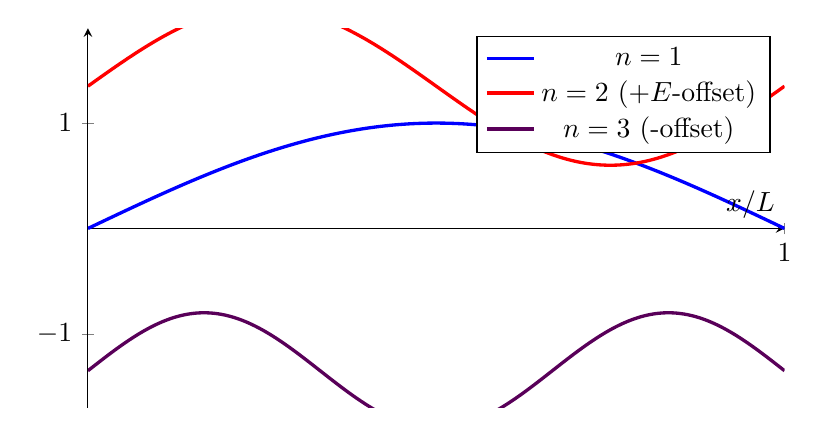
\begin{tikzpicture}
\begin{axis}[width=0.86\linewidth,height=6.4cm,xlabel={$x/L$},ylabel={},
 axis lines=middle,domain=0:1,samples=300,ymin=-1.7,ymax=1.9,xtick={0,1}]
 \addplot[blue,very thick,domain=0:1]{sin(deg(pi*x))};
 \addlegendentry{$n=1$};
 \addplot[red,very thick,domain=0:1]{sin(deg(2*pi*x))*0.75+1.35};
 \addlegendentry{$n=2$ (+$E$-offset)};
 \addplot[violet!70!black,very thick,domain=0:1]{sin(deg(3*pi*x))*0.55-1.35};
 \addlegendentry{$n=3$ (-offset)};
\end{axis}
\end{tikzpicture}
\caption{અનંત કૂવાનાં $\psi_n$; નોડો $n-1$ સંખ્યામાં.}
\end{figure}

\subsection*{આકૃતિ 4.2 : પગથિયું અને અવરોધ — સ્થિતિઊર્જા ચિત્રો}
\begin{figure}[htbp]
\centering
\begin{tikzpicture}[scale=0.95]
 \draw[thick,-Stealth] (-3.5,0) -- (3.5,0);
 % step
 \draw[blue,very thick] (-3.5,0.15) -- (0,0.15) -- (0,1.6) -- (3.5,1.6);
 \node[blue] at (-2,0.45) {$V=0$};
 \node[blue] at (2.2,1.85) {$V=V_0$};
 \draw[dashed,red] (-3.5,0.9) node[left] {$E>V_0$} -- (3.5,0.9);
 \node at (0,-0.4) {(a) પગથિયું};
 % barrier
 \begin{scope}[shift={(0,-3.4)}]
 \draw[thick,-Stealth] (-3.5,0) -- (3.5,0);
 \fill[orange!30] (-0.8,0.15) rectangle (0.8,1.9);
 \draw[orange!70!black,very thick] (-3.5,0.15) -- (-0.8,0.15) -- (-0.8,1.9) -- (0.8,1.9) -- (0.8,0.15) -- (3.5,0.15);
 \node[orange!70!black] at (0,2.15) {$V_0$};
 \draw[<->] (-0.8,-0.25) -- node[below]{$L$} (0.8,-0.25);
 \draw[dashed,red] (-3.5,0.8) node[left] {$E<V_0$} -- (3.5,0.8);
 \node at (0,-0.75) {(b) અવરોધ — ટનલિંગ};
 \end{scope}
\end{tikzpicture}
\caption{પગથિયું અને અવરોધ સ્થિતિઊર્જા સંરચનાઓ.}
\end{figure}

\subsection*{આકૃતિ 4.3 : ટનલિંગ — $T$ vs $L$ (ઘાતાંકીય)}
\begin{figure}[htbp]
\centering
\begin{tikzpicture}
\begin{axis}[width=0.62\linewidth,height=5.6cm,xlabel={$L$ (Å)},ylabel={$T$ (પ્રમાણભૂત)},
 axis lines=box,domain=0:10,samples=120,ymin=0]
 \addplot[blue,very thick]{exp(-1.05*x)};
 \addplot[red,dashed,very thick]{exp(-0.52*x)};
 \legend{ઇલેક્ટ્રોન ($V_0-E=2$ eV), પ્રોટોન (હલકો ઢાળ)}
\end{axis}
\end{tikzpicture}
\caption{$T\propto e^{-2\alpha L}$ — પહોળાઈ/દળ વધે તો ટનલિંગ પ્રચંડ રીતે ઘટે.}
\end{figure}

\subsection*{આકૃતિ 4.4 : STMનું સ્કીમેટિક}
\begin{figure}[htbp]
\centering
\begin{tikzpicture}[scale=1.0]
 \draw[very thick,gray] (0,2.6) -- (0.5,2.0) -- (0.5,1.55) -- (0.42,1.45);
 \node[right] at (0.6,2.4) {ટંગસ્ટન ટિપ};
 \draw[thick,fill=gray!25] (-1.6,-0.4) rectangle (2.4,0);
 \node[below] at (0.4,-0.45) {વાહક નમૂનો};
 \draw[-Stealth,cyan!60!black,dashed,very thick] (0.46,1.4) -- (0.46,0.05);
 \node[cyan!60!black,left] at (0.4,0.7) {$I\propto e^{-2\kappa z}$};
 \draw[<->,red] (0.75,1.4) -- node[right]{$z$} (0.75,0.02);
 \draw[thick] (0.5,2.0) -- (0.5,3.1);
 \draw[thick,-Stealth] (0.5,3.1) -- (0.5,3.5); \node[right] at (0.55,3.3) {પાઇઝો-સ્કેનર};
 \draw[thick] (-2.6,0.6) circle[radius=0.32]; \node[left] at (-2.95,0.6) {$I$ માપન};
 \draw[thick] (-2.28,0.6) -- (0.44,0.9);
 \draw[thick] (2.4,-0.2) -- (3.2,-0.2) -- (3.2,1.2);
 \draw (3.2,1.2) -- (3.2,1.6); \node[right] at (3.28,1.4) {$V_b$};
\end{tikzpicture}
\caption{STM: ટનલ-ધારાની ઘાતાંકીય દૂર-સંવેદનશીલતાથી પરમાણુ-ટોપોગ્રાફી.}
\end{figure}

\subsection*{આકૃતિ 4.5 : હાર્મોનિક દોલક — સ્થિતિઊર્જા અને સ્તરો}
\begin{figure}[htbp]
\centering
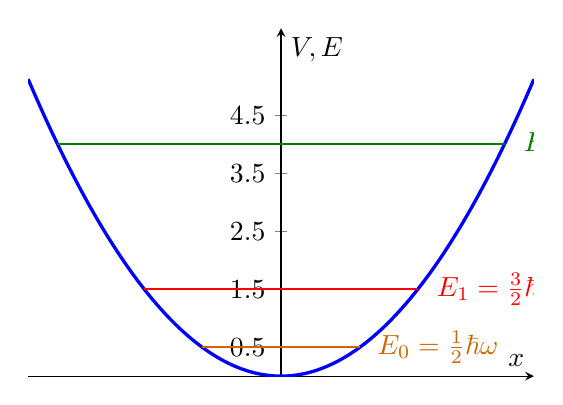
\begin{tikzpicture}
\begin{axis}[width=0.66\linewidth,height=6cm,xlabel={$x$},ylabel={$V,E$},
 axis lines=middle,domain=-3.2:3.2,samples=200,ymin=0,ymax=6,
 xtick=\empty,ytick={0.5,1.5,2.5,3.5,4.5}]
 \addplot[blue,very thick]{0.5*x*x};
 \draw[green!50!black,thick] (-2.83,4.0) -- (2.83,4.0);
 \draw[red,thick] (-1.73,1.5) -- (1.73,1.5);
 \draw[orange!80!black,thick] (-1.0,0.5) -- (1.0,0.5);
 \node[orange!80!black,right] at (1.1,0.5) {$E_0=\tfrac12\hbar\omega$};
 \node[red,right] at (1.85,1.5) {$E_1=\tfrac32\hbar\omega$};
 \node[green!50!black,right] at (2.95,4.0) {$E_3$};
\end{axis}
\end{tikzpicture}
\caption{દોલકની પરવલયિક સ્થિતિઊર્જા અને સમાન-અંતર ઊર્જા-સિડી $(n+\tfrac12)\hbar\omega$.}
\end{figure}

\section{સંપૂર્ણ ઉકેલેલા દાખલા}
\begin{dahlo}{દાખલો 4.1 : કૂવાની ભૂમિ-ઊર્જા}
ઇલેક્ટ્રોન $L=1$ Å કૂવામાં બંધનિત છે. $E_1$ અને $E_2$ ગણો.
\tcblower
\textbf{ઉકેલ:} $\dfrac{\pi^{2}\hbar^{2}}{2mL^{2}}=\dfrac{9.87\times(1.055\times10^{-34})^{2}}{2\times9.11\times10^{-31}\times10^{-20}}=6.03\times10^{-18}$ J $=37.6$ eV.
$E_1=37.6$ eV; $E_2=4E_1=150.4$ eV; સંક્રમણ ઊર્જા $112.8$ eV (XUV પ્રદેશ).
\end{dahlo}

\begin{dahlo}{દાખલો 4.2 : 3D બોક્સની ક્ષીણતા}
ઘન બોક્સમાં $E=14E_0$ ઊર્જાની કેટલી અવસ્થાઓ? ($E_0=\pi^2\hbar^2/2mL^2$)
\tcblower
\textbf{ઉકેલ:} $n_x^{2}+n_y^{2}+n_z^{2}=14$ શોધીએ: $1^{2}+2^{2}+3^{2}=14$. ક્રમ-વિનિમય: $(1,2,3)$ નાં $3!=6$ ક્રમ. એટલે $g=6$.
(સરખામણી: $E=6E_0\Rightarrow g=3$; $E=3E_0\Rightarrow(1,1,1)\Rightarrow g=1$.)
\end{dahlo}

\begin{dahlo}{દાખલો 4.3 : પરિમિત કૂવામાં પ્રસરણ અંતર}
ઇલેક્ટ્રોનની ઊર્જા $V_0-E=1$ eV હોય તો પ્રસરણ અંતર $\delta=1/\alpha$ ગણો.
\tcblower
\textbf{ઉકેલ:} $\alpha=\sqrt{2m(V_0-E)}/\hbar$
\[
=\frac{\sqrt{2\times9.11\times10^{-31}\times1.602\times10^{-19}}}{1.055\times10^{-34}}
=\frac{5.40\times10^{-25}}{1.055\times10^{-34}}=5.12\times10^{9}\ \mathrm{m}^{-1}.
\]
$\delta=1/\alpha=1.95\times10^{-10}$ m $\approx2$ Å — પરમાણુ-ક્રમનું પ્રસરણ!
\end{dahlo}

\begin{dahlo}{દાખલો 4.4 : પગથિયું $E>V_0$ માટે $R,T$}
ઇલેક્ટ્રોન $E=5$ eV, $V_0=4$ eV પગથિયા પર પડે. $R$ અને $T$ ગણો.
\tcblower
\textbf{ઉકેલ:} $k\propto\sqrt{E-V}$ ધારવાથી $k_2/k_1=\sqrt{(5-4)/5}=0.447$.
\[
R=\left(\frac{1-0.447}{1+0.447}\right)^{2}=\left(\frac{0.553}{1.447}\right)^{2}=0.146,
\qquad
T=\frac{4(0.447)}{(1.447)^{2}}=0.854 .
\]
શાસ્ત્રીય ભવિષ્યવાણી $R=0$; ક્વોન્ટમ $R\approx15\%$ — ઊર્જા સંરક્ષણ સાથે $R+T=1$. ✓
\end{dahlo}

\begin{dahlo}{દાખલો 4.5 : ટનલિંગ સંભાવના}
ઇલેક્ટ્રોન $E=2$ eV, $V_0=5$ eV, $L=10$ Å અવરોધ પાર કરે તો $T$ ગણો.
\tcblower
\textbf{ઉકેલ:} $V_0-E=3$ eV:
\[
\alpha=\frac{\sqrt{2\times9.11\times10^{-31}\times3\times1.602\times10^{-19}}}{1.055\times10^{-34}}
=8.87\times10^{9}\ \mathrm{m}^{-1};
\qquad 2\alpha L=2(8.87\times10^{9})(10^{-9})=17.74 .
\]
પૂર્વ-ગુણક: $\dfrac{16E(V_0-E)}{V_0^{2}}=\dfrac{16\times2\times3}{25}=3.84$:
\[
T=3.84\times e^{-17.74}=3.84\times1.97\times10^{-8}=7.6\times10^{-8}.
\]
એટલે લગભગ $1.3\times10^{7}$ ઇલેક્ટ્રોનમાંથી એક જ પાર જાય — છતાં STM માં આ જ પ્રક્રિયા nA ધારા આપે!
\end{dahlo}

\begin{dahlo}{દાખલો 4.6 : $\alpha$-ક્ષયની આયુ-સંવેદનશીલતા}
ગામોવ સિદ્ધાંત મુજબ $T\sim e^{-2G}$. $2G$ 30 થી 31 થાય તો આયુ કેટલા ગણી બદલાય?
\tcblower
\textbf{ઉકેલ:} આયુ $t\propto1/T\sim e^{+2G}$: ગુણોત્તર $=e^{31-30}=e\approx2.72$.
એક એકમનો ફેરફાર ≈ ત્રણ-ગણ આયુ-ફેરફાર; $^{238}$U જેવાં ન્યુક્લાઇડમાં $2G\approx90$ ⇒ આયુ $10^{17}$ s (અર્ધ-આયુ $4.5\times10^{9}$ વર્ષ) — નાના $G$-ફેરફારો મહાકલ્પીય તફાવત કરે.
\end{dahlo}

\begin{dahlo}{દાખલો 4.7 : STM ધારા-સંવેદનશીલતા}
ટિપ–સપાટી અંતર $1$ nm થી $1.2$ nm થાય તો ટનલ ધારા કેટલા ગણી બદલાય? ($\kappa\approx10^{10}\ \mathrm{m}^{-1}$)
\tcblower
\textbf{ઉકેલ:} $I\propto e^{-2\kappa z}$:
\[
\frac{I_2}{I_1}=e^{-2\kappa(z_2-z_1)}=e^{-2\times10^{10}\times0.2\times10^{-9}}=e^{-4}=0.018 .
\]
ધારા ≈ 55 ગણી ઘટે — એક હાઇડ્રોજન પરમાણુ જેટલા (0.2 nm) અંતર-ફેરફારથી ધારામાં પ્રચંડ ફેરફાર.
\end{dahlo}

\begin{dahlo}{દાખલો 4.8 : દોલકનું ભૂમિ-તરંગ વિધેય}
$\psi_0=N_0e^{-\xi^{2}/2}$ પ્રમાણિત કરો અને $N_0$ શોધો ($a\equiv\sqrt{\hbar/m\omega}$).
\tcblower
\textbf{ઉકેલ:} $\xi=x/a$, $P=N_0^{2}e^{-x^{2}/a^{2}}$:
\[
1=N_0^{2}\int_{-\infty}^{\infty}e^{-x^{2}/a^{2}}\dd x=N_0^{2}\,a\sqrt{\pi}
\Rightarrow N_0=\frac{1}{(\pi a^{2})^{1/4}}=\frac{1}{\pi^{1/4}\sqrt{a}} .
\]
તપાસ: TISE માં $\psi_0$ રાખતાં $E_0=\hbar\omega/2$ મળે — શૂન્ય-બિંદુ ઊર્જા ફરી પુષ્ટ.
\end{dahlo}

\begin{dahlo}{દાખલો 4.9 : હાઇડ્રોજનનાં અવસ્થા-ગણતરી}
$n=3$ અવસ્થા માટે (a) શક્ય $\ell$ મૂલ્યો, (b) દરેક $\ell$ માટે $m_\ell$, (c) કુલ ક્ષીણતા (સ્પિન વિના) શોધો.
\tcblower
\textbf{ઉકેલ:} (a) $\ell=0,1,2$.
(b) $\ell=0$: $m_\ell=0$ (1 અવસ્થા); $\ell=1$: $m_\ell=-1,0,+1$ (3); $\ell=2$: $m_\ell=-2..+2$ (5).
(c) કુલ $=1+3+5=9=n^{2}$. ✓ સ્પિન સહિત $g=18$.
\end{dahlo}

\begin{dahlo}{દાખલો 4.10 : હાઇડ્રોજન સંક્રમણ તરંગલંબાઈ}
$n=4\to n=2$ સંક્રમણની ઉત્સર્જિત તરંગલંબાઈ ગણો.
\tcblower
\textbf{ઉકેલ:} $E_4=-13.6/16=-0.85$ eV; $E_2=-3.40$ eV; $\Delta E=2.55$ eV.
\[
\lambda=\frac{1240\ \text{eV·nm}}{2.55\ \text{eV}}=486\ \text{nm}.
\]
આ જ પ્રખ્યાત બેલ્મર H$\beta$ નીલમ રેખા છે.
\end{dahlo}

\section{સ્વાધ્યાય}

\subsection{વૈચારિક પ્રશ્નો}
\begin{enumerate}[label=\textbf{Q\arabic*.}]
  \item અનંત કૂવાની ઊર્જા શા માટે અસતત છે જ્યારે મુક્ત કણની સતત?
  \item કૂવાની પહોળાઈ ઘટાડવાથી ઊર્જા-સ્તરો પર શું થાય?
  \item 3D બોક્સમાં ક્ષીણતા 1D કેમ નથી?
  \item પરિમિત કૂવાનાં ઊર્જા-સ્તરો અનંત કૂવા કરતાં નાના કેમ?
  \item $E>V_0$ પગથિયા પર પરાવર્તન શાસ્ત્રીય અંતર્દૃષ્ટિને કેવી રીતે વિરોધાભાસી છે?
  \item ટનલિંગ દર પર દળ અને અવરોધ-પહોળાઈની ઘાતાંકીય અસર સમજાવો.
  \item STM માં ધારા કેમ 'પરમાણુ-ઊંચાઈ' માપે છે?
  \item શૂન્ય-બિંદુ ઊર્જા દોલકમાં અનિશ્ચિતતા સિદ્ધાંતથી કેમ અનિવાર્ય છે?
  \item હાઇડ્રોજનમાં $n$ જ ઊર્જા નક્કી કરે પણ $\ell,m_\ell$ કેમ જરૂરી?
  \item કૂલુંબ-અવરોધનું ટનલિંગ સૂર્યનાં ફ્યુઝન માટે કેમ અનિવાર્ય છે?
\end{enumerate}

\subsection{અણઉકેલેલા દાખલા}
\begin{enumerate}[label=\textbf{P\arabic*.}]
  \item ઇલેક્ટ્રોન, $L=2$ Å કૂવાની $E_1$ ગણો. \hfill [\textbf{જવાબ:} $9.4$ eV]
  \item P1 માં $n=3\to1$ સંક્રમણ ફોટોનનું $\lambda$ ગણો. \hfill [\textbf{જવાબ:} $\approx11$ nm]
  \item ઘન બોક્સમાં $E=12E_0$ ની ક્ષીણતા ગણો. \hfill [\textbf{જવાબ:} $g=1$ ($(2,2,2)$)]
  \item $V_0-E=2$ eV ઇલેક્ટ્રોન માટે $\delta$ ગણો. \hfill [\textbf{જવાબ:} $\approx1.4$ Å]
  \item $E=6$ eV, $V_0=4$ eV પગથિયાનું $R$ ગણો. \hfill [\textbf{જવાબ:} $\approx0.036$]
  \item $E=3$ eV, $V_0=6$ eV, $L=5$ Å અવરોધનું $T$ ગણો. \hfill [\textbf{જવાબ:} $\sim10^{-5}$ ક્રમ]
  \item STM અંતર $0.5\to0.6$ nm: ધારા-ગુણોત્તર ($\kappa=10^{10}$). \hfill [\textbf{જવાબ:} $\approx0.135$]
  \item દોલક $n=2$ નાં નોડ-સંખ્યા અને ઊર્જા લખો. \hfill [\textbf{જવાબ:} 2 નોડ; $E_2=\tfrac52\hbar\omega$]
  \item હાઇડ્રોજન $n=2$: ક્ષીણતા (સ્પિન સહિત) ગણો. \hfill [\textbf{જવાબ:} $8$]
  \item હાઇડ્રોજન $n=3\to2$ સંક્રમણ $\lambda$ ગણો. \hfill [\textbf{જવાબ:} $656$ nm (H$\alpha$)]
\end{enumerate}

\section{50 ઉચ્ચ સ્તરીય MCQs}

\begin{enumerate}[label=\textbf{\arabic*.}]
  \item અનંત કૂવાની ઊર્જા $E_n\propto$ ? (A) $n$ (B) $n^{2}$ (C) $n^{3}$ (D) $1/n$
  \item કૂવાની ભૂમિ-અવસ્થા ઊર્જા: (A) 0 (B) $\pi^{2}\hbar^{2}/2mL^{2}$ (C) $\infty$ (D) $\hbar^{2}/2mL^{2}$
  \item $\psi_n$ નાં નોડ (કૂવા અંદર): (A) $n$ (B) $n-1$ (C) $n+1$ (D) $2n$
  \item કૂવાની પહોળાઈ અડધી થાય તો $E_1$: (A) અડધું (B) બમણું (C) ચાર-ગણું (D) અપરિવર્તિત
  \item પ્રમાણિત $\psi_n$ નો $A=$ ? (A) $1/\sqrt L$ (B) $\sqrt{2/L}$ (C) $2/L$ (D) $\sqrt{L/2}$
  \item 3D ઘન બોક્સ $E=6E_0$ ની ક્ષીણતા: (A) 1 (B) 3 (C) 6 (D) 9
  \item 3D ઘન બોક્સ $E=3E_0$ ની ક્ષીણતા: (A) 1 (B) 3 (C) 6 (D) 8
  \item પરિમિત કૂવાનાં ઊર્જા-સ્તરો મળે છે: (A) બીજગણિતથી (B) અતિચલાંકીય સમીકરણોના સંખ્યાત્મક ઉકેલથી (C) અનંત-કૂવા જેવા જ (D) શૂન્ય
  \item પ્રસરણ અંતર $\delta=$ ? (A) $\hbar/\sqrt{2m(V_0-E)}$ (B) $\sqrt{2mV_0}/\hbar$ (C) $\alpha$ (D) $2\alpha L$
  \item કૂવાની બહાર $|\psi|$ નું સ્વરૂપ: (A) દોલાતું (B) ઘાતાંકીય ક્ષય (C) રેખીય (D) શૂન્ય
  \item $E>V_0$ પગથિયા પર ક્વોન્ટમ પરિણામ: (A) $R=0$ (B) $R>0$ (C) $T=0$ (D) $R=1$
  \item પગથિયું $E\to V_0$ (ઉપરથી) મર્યાદામાં $R\to$ ? (A) 0 (B) 1 (C) 0.5 (D) $\infty$
  \item પગથિયું $E\gg V_0$ માં $R\approx$ ? (A) 1 (B) 0.5 (C) $\approx0$ (D) $V_0/E$
  \item $E<V_0$ અનંત પગથિયા માટે $T=$ ? (A) $e^{-2\alpha L}$ (B) 0 (C) 1 (D) $V_0/E$
  \item અવરોધ ટનલિંગ $T\approx$ ? (A) $e^{-2\alpha L}$ (B) $e^{+2\alpha L}$ (C) $\alpha L$ (D) $1/\alpha L$
  \item $\alpha=$ ? (A) $\sqrt{2m(E-V_0)}/\hbar$ (B) $\sqrt{2m(V_0-E)}/\hbar$ (C) $2mV_0/\hbar$ (D) $\hbar/\sqrt{2mV_0}$
  \item અવરોધ-પહોળાઈ બમણી થાય તો $T$ લગભગ: (A) બમણું (B) અડધું (C) $T$ નું વર્ગ ઘટે ($e^{-4\alpha L}$) (D) અપરિવર્તિત
  \item ગામોવ સિદ્ધાંત સમજાવે છે: (A) ફોટોવિદ્યુત અસર (B) $\alpha$-ક્ષયની આયુ (C) લેસર (D) સુપરકંડક્ટન્સ
  \item $\alpha$-ક્ષયમાં કણ કેવી રીતે છટકે? (A) કૂલુંબ-અવરોધનું ટનલિંગ (B) ગુરુત્વ (C) ફોટોન શોષણ (D) માગ્નેટિક ક્ષેત્ર
  \item Geiger-Nuttall નિયમ સંકળાયેલ: (A) $\alpha$-ક્ષય આયુ–ઊર્જા (B) β-વર્ણપટ (C) γ-શોષણ (D) ફ્યુઝન-દર
  \item STM ના શોધક: (A) બેલ-બિનિંગ (B) બિનિંગ-રોહરર (C) ડેવિસન-જર્મર (D) થોમસન
  \item STM ધારા સ્વરૂપ: (A) $e^{-2\kappa z}$ (B) $z^{2}$ (C) $1/z$ (D) $e^{+2\kappa z}$
  \item ટનલ ડાયોડની વિશિષ્ટ વિશેષતા: (A) ધન પ્રતિરોધ (B) નેગેટિવ ડિફરેન્શિયલ રેઝિસ્ટન્સ (C) અનંત પ્રતિરોધ (D) શૂન્ય ધારા
  \item ફ્લેશ મેમરીમાં ચાર્જ-ઇન્જેક્શન પ્રક્રિયા: (A) થર્મિયોનિક (B) ફોવલર-નોર્ધામ ટનલિંગ (C) ફોટોવિદ્યુત (D) કૉમ્પ્ટન
  \item દોલકની ઊર્જા સિડી: (A) સમાન-અંતર $\hbar\omega$ (B) $n^{2}$ પ્રમાણે (C) સતત (D) $1/n^{2}$
  \item દોલકની શૂન્ય-બિંદુ ઊર્જા: (A) 0 (B) $\hbar\omega$ (C) $\hbar\omega/2$ (D) $3\hbar\omega/2$
  \item દોલક તરંગ-વિધેયમાં બહુપદી: (A) લાગ્યુર (B) હર્માઇટ (C) લેજાન્ડર (D) ચેબિશેવ
  \item $H_2(\xi)=$ ? (A) $2\xi$ (B) $4\xi^{2}-2$ (C) $1$ (D) $8\xi^{3}-12\xi$
  \item દોલકની ભૂમિ-અવસ્થાનાં નોડ: (A) 0 (B) 1 (C) 2 (D) $\infty$
  \item હાઇડ્રોજન ઊર્જા $E_n$ આધારિત છે: (A) ફક્ત $n$ પર (B) ફક્ત $\ell$ પર (C) $m_\ell$ પર (D) ત્રણેય પર
  \item હાઇડ્રોજન માટે શક્ય $\ell$: (A) $\ell<n$ (B) $\ell\le n$ (C) $\ell>n$ (D) $\ell=n^{2}$
  \item હાઇડ્રોજન માટે શક્ય $m_\ell$: (A) $|m_\ell|\le\ell$ (B) $|m_\ell|\le n$ (C) કોઈપણ પૂર્ણાંક (D) $\pm1$
  \item સ્પિન ક્વોન્ટમ સંખ્યા $m_s=$ ? (A) $\pm\tfrac12$ (B) $0,1$ (C) $\pm1$ (D) $n$
  \item હાઇડ્રોજન $n$-અવસ્થાની ક્ષીણતા (સ્પિન વિના): (A) $n$ (B) $2n^{2}$ (C) $n^{2}$ (D) $n^{3}$
  \item હાઇડ્રોજન ભૂમિ-અવસ્થાની $\ell$: (A) 0 (B) 1 (C) $n-1$ (D) કોઈ નહીં
  \item બેલ્મર H$\alpha$ ($656$ nm) સંક્રમણ: (A) $3\to2$ (B) $4\to2$ (C) $2\to1$ (D) $5\to2$
  \item લાયમન શ્રેણી પ્રદેશ: (A) IR (B) દૃશ્ય (C) UV (D) X-ray
  \item કૂવાની ઊર્જા-સ્પેસિંગ મોટા $n$ પર: (A) વધે (B) ઘટે અને લગભગ સતત જેવી (C) અચલાંક (D) અનંત
  \item અનંત કૂવાની સીમા પર $\psi$: (A) મહત્તમ (B) 0 (C) અનંત (D) $1/L$
  \item પગથિયા પર $\psi$ અને $\psi'$: (A) અસતત (B) સતત (C) એક જ સતત (D) શૂન્ય
  \item ટનલિંગ શા માટે શાસ્ત્રીયમાં અશક્ય? (A) $E<V_0$ પ્રદેશમાં $p$ કાલ્પનિક (B) ઊર્જા અભાવ (C) દળ વધુ (D) ઝડપ ઓછી
  \item ટનલિંગની સંભાવના સૌથી વધુ જ્યારે: (A) દળ ઓછો, અવરોધ પાતળો (B) દળ મોટો (C) અવરોધ પહોળો (D) ઊર્જા નાની
  \item ક્વોન્ટમ કૂવા-લેસરનું સિદ્ધાંત-આધાર: (A) અનંત કૂવાની અસતત સ્તરો (સ્તર-સંરચના) (B) ટનલિંગ (C) સ્પિન (D) ક્ષીણતા
  \item હાઇડ્રોજન રેડિયલ સંભાવના મહત્તમ (ભૂમિ-અવસ્થા) ત્રિજ્યા: (A) $a_0$ (B) $2a_0$ (C) $a_0/2$ (D) $4a_0$
  \item દોલકમાં શાસ્ત્રીય-ટર્નિંગ બિંદુ એટલે: (A) $V=E$ (B) $V=0$ (C) $\psi=0$ (D) નોડ
  \item WKB ટનલિંગ અંદાજ $T\sim$: (A) $e^{-2\int\alpha dx}$ (B) $\int\alpha dx$ (C) $e^{+\int\alpha dx}$ (D) $\alpha^{2}$
  \item અનંત કૂવામાં $\langle x\rangle$ ($0<x<L$): (A) $0$ (B) $L/2$ (C) $L$ (D) $nL/\pi$
  \item પરિમિત કૂવો જેટલો ઊંડો તેનાં સ્તરો: (A) અનંત કૂવા જેવા (B) અનંત કૂવા કરતાં ઓછા અને નાના ઊર્જા (C) વધુ (D) સતત
  \item હાઇડ્રોજન TISE ગોળીય નિર્દેશાંક કેમ? (A) સરળ ગણિત (B) સ્થિતિઊર્જા કેન્દ્રીય-સમિતિય (C) ક્વોન્ટમ નિયમ (D) સ્પિન જરૂરી
  \item $n=2$ હાઇડ્રોજન અવસ્થાની ઊર્જા: (A) $-13.6$ eV (B) $-3.4$ eV (C) $-1.51$ eV (D) $-0.85$ eV
\end{enumerate}

\subsection*{જવાબ ચાવી અને પગલાંવાર સમજૂતી}
\begin{javabchavi}{MCQ જવાબ ચાવી (એકમ 4)}
1-B | 2-B | 3-B | 4-C | 5-B | 6-B | 7-A | 8-B | 9-A | 10-B |
11-B | 12-B | 13-C | 14-B | 15-A | 16-B | 17-C | 18-B | 19-A | 20-A |
21-B | 22-A | 23-B | 24-B | 25-A | 26-C | 27-B | 28-B | 29-A | 30-A |
31-A | 32-A | 33-A | 34-C | 35-A | 36-A | 37-C | 38-B | 39-B | 40-B |
41-A | 42-A | 43-A | 44-A | 45-A | 46-B | 47-A | 48-B | 49-B | 50-B
\end{javabchavi}

\begin{javabchavi}{MCQ પગલાંવાર સમજૂતી (મુખ્ય ગણતરી-આધારિત પ્રશ્નો)}
\begin{description}[style=nextline,itemsep=0pt]
  \item[4.] $E_1\propto1/L^{2}$; $L\to L/2$ ⇒ $E_1\to4E_1$.
  \item[6./7.] $n_x^{2}+n_y^{2}+n_z^{2}$: $6=(1,1,\sqrt4)=(1,1,2)$ ત્રણ ક્રમ ⇒ $g=3$; $3=(1,1,1)$ ⇒ $g=1$.
  \item[9.] $\delta=1/\alpha=\hbar/\sqrt{2m(V_0-E)}$ — $|\psi|$ નું $e^{-1}$ ભાગનું અંતર.
  \item[11.] $E>V_0$: $R=\big((k_1-k_2)/(k_1+k_2)\big)^{2}>0$ જ્યારે $k_2\neq k_1$ — ક્વોન્ટમ પરાવર્તન.
  \item[12.] $E\to V_0$: $k_2\to0$ ⇒ $R\to1$ — સંપૂર્ણ પરાવર્તન મર્યાદા.
  \item[17.] $L\to2L$: $e^{-2\alpha(2L)}=(e^{-2\alpha L})^{2}$ — વર્ગ ઘટાડો.
  \item[34.] સ્પિન વિના ક્ષીણતા $=\sum_{\ell=0}^{n-1}(2\ell+1)=n^{2}$.
  \item[36.] બેલ્મર H$\beta$: $E_4-E_2=-0.85-(-3.40)=2.55$ eV ⇒ $486$ nm; H$\alpha$ છે $3\to2$.
  \item[44.] ભૂમિ-અવસ્થાની રેડિયલ સંભાવના $P(r)=4r^{2}|\psi_{100}|^{2}/a_0^{3}$ નું મહત્તમ $r=a_0$ પર.
\end{description}
શેષ પ્રશ્નો સૂત્ર-વ્યાખ્યા આધારિત; \S4.2--\S4.3 સાથે સરખાવો.
\end{javabchavi}

% ============================================================================
% UNIT 5 : આધુનિક ક્વોન્ટમ તકનીકી, આંકડાશાસ્ત્ર અને એન્જિનિયરિંગ અનુપ્રયોગો
% ============================================================================
\chapter{આધુનિક ક્વોન્ટમ તકનીકી, આંકડાશાસ્ત્ર અને એન્જિનિયરિંગ અનુપ્રયોગો \en{Modern Quantum Technologies, Statistics and Engineering Applications}}

\section{પ્રસ્તાવના અને શૈક્ષણિક ઉદ્દેશ્યો}
\begin{uddeshyo}
આ એકમના અભ્યાસ પછી વિદ્યાર્થી:
\begin{enumerate}[label=\textbf{(\arabic*)}]
  \item કાળ-સ્વતંત્ર અ-ક્ષીણ (Non-degenerate) ક્ષોભ સિદ્ધાંત (Perturbation Theory)નાં પ્રથમ-ક્રમ સુધારા તારવી શકશે.
  \item સમાન કણો, સમમિતીકરણ અને પૌલી બહિષ્કાર નિયમ (Pauli Exclusion Principle) સમજી શકશે.
  \item બોઝ-આઇન્સ્ટાઇન, ફર્મી-ડિરાક અને બોલ્ટ્ઝમાન વિતરણો સરખાવી શકશે; $E_F$ ગણી શકશે.
  \item ક્વોન્ટમ અવરોધન (Quantum Confinement) — 2D કૂવા, 1D વાયર, 0D ડોટ — અને અવસ્થા-ઘનતા (Density of States) વિશ્લેષણ કરી શકશે.
  \item લેસર ભૌતિકી — પ્રેરિત ઉત્સર્જન, આઇન્સ્ટાઇન $A,B$ ગુણાંક, વસ્તી ઉલટાણ, રૂબી અને He-Ne લેસર — સમજાવી શકશે.
  \item ક્યુબિટ, બ્લોચ ગોળો, બેલ અવસ્થાઓ, ક્વોન્ટમ ગેટો અને BB84 ક્રિપ્ટોગ્રાફી સમજી/ઉપયોગ કરી શકશે.
\end{enumerate}
\end{uddeshyo}

\section{વિસ્તૃત સૈદ્ધાંતિક વિવરણ}

\subsection{ક્ષોભ સિદ્ધાંત : પ્રથમ-ક્રમ અ-ક્ષીણ \en{First-Order Non-degenerate Perturbation Theory}}
ખરો હેમિલ્ટોનિયન $\hat H=\hat H_0+\lambda\hat H'$ ($\hat H'$ = નાનું ક્ષોભ). $\hat H_0$ નાં જ્ઞાત ઉકેલ: $\hat H_0|n^{(0)}\rangle=E_n^{(0)}|n^{(0)}\rangle$. શક્તિ-શ્રેણી ધારણ:
\[
E_n=E_n^{(0)}+\lambda E_n^{(1)}+\cdots,\qquad
|n\rangle=|n^{(0)}\rangle+\lambda|n^{(1)}\rangle+\cdots .
\]
$\lambda$ નાં ગુણકોની સરખામણીથી પ્રથમ-ક્રમ:
\begin{equation}
\boxed{\;E_n^{(1)}=\langle n^{(0)}|\hat H'|n^{(0)}\rangle\;}
\label{eq:perturb}
\end{equation}
— એટલે \emph{ક્ષોભનું અપેક્ષિત મૂલ્ય} જ ઊર્જા-સુધારો. ઉદાહરણ: દોલકમાં સ્થિર વિદ્યુત ક્ષેત્ર (Stark) અથવા કૂવામાં નાનું $V_1x$.

\subsection{સમાન કણો અને પૌલી બહિષ્કાર નિયમ \en{Identical Particles and Pauli Principle}}
બે સમાન કણોની અવસ્થા અવલોકન-અર્થઘટન માટે કણ-વિનિમય હેઠળ સમમિત હોવી જ જોઈએ:
\[
\Psi_{\pm}(q_1,q_2)=\frac{1}{\sqrt2}\big[\psi_a(q_1)\psi_b(q_2)\pm\psi_a(q_2)\psi_b(q_1)\big]:
\]
\begin{center}
\begin{tabular}{@{}lll@{}}
\toprule
કણ-પ્રકાર & સમમિતિ & આંકડાશાસ્ત્ર \\
\midrule
બોસોન (સ્પિન $0,1,2\dots$) & $+$ સમમિત & બોઝ-આઇન્સ્ટાઇન \\
ફર્મિઓન (અર્ધ સ્પિન) & $-$ પ્રતિસમમિત & ફર્મી-ડિરાક \\
\bottomrule
\end{tabular}
\end{center}
ફર્મિઓન માટે $\psi_a=\psi_b$ હોય તો $\Psi_{-}=0$ ⇒ એક ક્વોન્ટમ અવસ્થામાં બે સમાન ફર્મિઓન ન રહી શકે — \textbf{પૌલી બહિષ્કાર નિયમ}. આ જ નિયમ આવર્તન કોષ્ટક, ઇલેક્ટ્રોન વાયુ અને અર્ધવાહક બેન્ડ-રચનાનો મૂળ છે.

\subsection{ક્વોન્ટમ આંકડાશાસ્ત્ર \en{Quantum Statistics}}
ઊર્જા $E$ અવસ્થાની સરેરાશ વસ્તી:
\begin{equation}
f(E)=\frac{1}{e^{(E-\mu)/k_BT}\pm1}:\quad
\begin{cases}
+1:&\text{ફર્મી-ડિરાક},\\
-1:&\text{બોઝ-આઇન્સ્ટાઇન},
\end{cases}
\qquad
f_{MB}=e^{-(E-\mu)/k_BT}.
\label{eq:stats}
\end{equation}
ધાતુનાં ઇલેક્ટ્રોન માટે $T=0$: $f(E)=1$ જો $E<E_F$; $f(E)=0$ જો $E>E_F$, જ્યાં
\begin{equation}
E_F=\frac{\hbar^{2}}{2m}\left(3\pi^{2}n\right)^{2/3}
\qquad(n=\text{ઇલેક્ટ્રોન ઘનતા})
\label{eq:fermi}
\end{equation}
— \textbf{ફર્મી ઊર્જા}. તાંબામાં $n=8.5\times10^{28}$ m$^{-3}$ ⇒ $E_F\approx7.0$ eV.

\subsection{ક્વોન્ટમ અવરોધન અને અવસ્થા-ઘનતા \en{Quantum Confinement and DOS}}
જ્યારે કોઈ પરિમાણ ડી બ્રોગ્લી તરંગલંબાઈ ક્રમનો હોય, ત્યારે તે દિશામાં ઊર્જા ક્વોન્ટાઇઝ થાય:
\begin{center}
\begin{tabular}{@{}lll@{}}
\toprule
સંરચના & સ્વતંત્ર દિશા & અવસ્થા-ઘનતા $\rho(E)$ \\
\midrule
3D બલ્ક & 3 & $\propto\sqrt{E}$ \\
2D ક્વોન્ટમ કૂવો & 2 & સિડી-આકાર (પગથિયાં) : પ્રતિ ઉપ-બેન્ડ અચલાંક \\
1D ક્વોન્ટમ વાયર & 1 & $\propto1/\sqrt{E-E_n}$ (વેન કાંટા) \\
0D ક્વોન્ટમ ડોટ & 0 & ડેલ્ટા-કાર્યો (પરમાણુ જેવાં અસતત સ્તરો) \\
\bottomrule
\end{tabular}
\end{center}
ડોટમાં ઊર્જા-અંતર $\Delta E\sim\pi^2\hbar^2/2mL^2$ ⇒ નાનું $L$ (નેનો-કણ) ⇒ વિશાળ બેન્ડ ગેપ ⇒ રંગ-ટ્યૂનિંગ (CdSe QD: 2–8 nm ⇒ નીલમ→લાલ).

\subsection{લેસર ભૌતિકી \en{LASER Physics}}
\textbf{LASER} = Light Amplification by Stimulated Emission of Radiation. ત્રણ પ્રક્રિયા (આવૃત્તિ $\nu=(E_2-E_1)/h$):
\begin{enumerate}[label=(\alph*)]
  \item શોષણ: દર $\propto B_{12}u(\nu)N_1$;
  \item સ્વસ્પંદિત (Spontaneous) ઉત્સર્જન: $A_{21}N_2$;
  \item \textbf{પ્રેરિત ઉત્સર્જન (Stimulated Emission)}: $B_{21}u(\nu)N_2$ — આગમન-તરંગ સાથે સમ-કલા, સમ-દિશા, સમ-ધ્રુવીકરણમાં ફોટોન-જોડી!
\end{enumerate}
આઇન્સ્ટાઇન તારણી (1917): થર્મલ સંતુલનમાં પ્લાંક વિતરણ મેળવવા હોય તો:
\begin{equation}
A_{21}/B_{21}=8\pi h\nu^{3}/c^{3},\qquad B_{12}=B_{21}
\label{eq:einsteinAB}
\end{equation}
— એટલે પ્રેરિત ઉત્સર્જન શક્ય જ છે અને ઉચ્ચ $\nu$ પર તે મુશ્કેલ ($\propto\nu^3$).
સામાન્ય સંતુલનમાં $N_2<N_1$; લેસર માટે \textbf{વસ્તી ઉલટાણ (Population Inversion)} $N_2>N_1$ જરૂરી — ત્રણ-સ્તર (રૂબી) અથવા ચાર-સ્તર (He-Ne, Nd:YAG) પંપિંગથી.
\begin{itemize}[itemsep=2pt]
  \item \textbf{રૂબી લેસર (1960, Maiman):} Al$_2$O$_3$+Cr$^{3+}$; ત્રણ-સ્તર; ગ્રીન ફ્લેશ-લેમ્પ પંપ → $694.3$ nm લાલ પલ્સ.
  \item \textbf{He-Ne લેસર:} ગેસ-વિસર્જન; He ની મેટાસ્થિર અવસ્થા Ne ને પંપ કરે (ઊર્જા-સ્થાનાંતર); ચાર-સ્તર; $632.8$ nm સતત CW.
\end{itemize}

\subsection{ક્વોન્ટમ કમ્પ્યુટિંગનાં પાયા \en{Foundations of Quantum Computing}}
\paragraph{ક્લાસિકલ બિટ vs ક્યુબિટ (Qubit):} બિટ $\in\{0,1\}$; ક્યુબિટ:
\begin{equation}
|\psi\rangle=\alpha|0\rangle+\beta|1\rangle,\qquad |\alpha|^{2}+|\beta|^{2}=1 .
\label{eq:qubit}
\end{equation}
$n$ ક્યુબિટ $2^{n}$ અવસ્થાઓની અધિસ્થિતિ એકસાથે ધરે છે.
\paragraph{બ્લોચ ગોળો (Bloch Sphere):} $|\psi\rangle=\cos(\theta/2)|0\rangle+e^{\ii\phi}\sin(\theta/2)|1\rangle$ — $(\theta,\phi)$ ગોળાનો બિંદુ; ઉત્તર ધ્રુવ $|0\rangle$, દક્ષિણ $|1\rangle$, વિષુવવૃત્ત સમાન-મિશ્રણ.
\paragraph{ગૂંથણ (Entanglement):} બેલ અવસ્થાઓ:
\[
|\Phi^{\pm}\rangle=\tfrac{1}{\sqrt2}(|00\rangle\pm|11\rangle),\qquad
|\Psi^{\pm}\rangle=\tfrac{1}{\sqrt2}(|01\rangle\pm|10\rangle),
\]
— કોઈ એકલ-ક્યુબિટ ઉત્પાદન $|\psi\rangle\otimes|\psi'\rangle$ તરીકે લખી ન શકાય; માપનનાં પરિણામો સંપૂર્ણ સહસંબંધિત.
\paragraph{ક્વોન્ટમ લૉજિક ગેટો:}
\[
X=\begin{pmatrix}0&1\\1&0\end{pmatrix},\quad
Z=\begin{pmatrix}1&0\\0&-1\end{pmatrix},\quad
H=\frac{1}{\sqrt2}\begin{pmatrix}1&1\\1&-1\end{pmatrix},\quad
CNOT:\ |c,t\rangle\to|c,\ t\oplus c\rangle .
\]
$H|0\rangle=(|0\rangle+|1\rangle)/\sqrt2$ — અધિસ્થિતિનું નિર્માણ; $H^2=I$. CNOT + H થી $|00\rangle$ માંથી $|\Phi^+\rangle$ બનાવાય.
\paragraph{BB84 ક્વોન્ટમ કી-વિતરણ (Bennett-Brassard, 1984):}
એલિસ યાદ્રચ્છિક રીતે $Z$-આધાર ($|0\rangle,|1\rangle$) કે $X$-આધાર ($|\pm\rangle$) માં બિટ મોકલે; બોબ યાદ્રચ્છિક આધારમાં માપે; પછી ખુલ્લા ચેનલ પર આધારોની સરખામણીથી સ્કિપ્ટ-બિટ્સ રાખે. ઈવનું મધ્યવર્તી-માપન નો-ક્લોનિંગ પ્રમેયને કારણે ત્રુટિ-દર વધારે (~25%) — શોધાય છે. સુરક્ષા ગણતરી-કઠિનતા પર નહીં, ભૌતિક નિયમો પર!

\section{સંપૂર્ણ ગાણિતિક સાબિતીઓ}

\subsection{$E_n^{(1)}=\langle n^{(0)}|\hat H'|n^{(0)}\rangle$ ની તારણી}
શક્તિ-શ્રેણી $\hat H|n\rangle=E_n|n\rangle$ માં રાખી $\lambda$ ગુણક સરખાવીએ:
\[
(\hat H_0-E_n^{(0)})|n^{(1)}\rangle=(E_n^{(1)}-\hat H')|n^{(0)}\rangle .
\]
ડાબી બાજુ $\langle n^{(0)}|$ થી આંતરિક ગુણાકાર: $\langle n^{(0)}|(\hat H_0-E_n^{(0)})=0$ (હર્મિટિયનત્વ):
\[
0=E_n^{(1)}-\langle n^{(0)}|\hat H'|n^{(0)}\rangle
\Rightarrow\boxed{E_n^{(1)}=\langle n^{(0)}|\hat H'|n^{(0)}\rangle .}
\]

\subsection{ફર્મી ઊર્જા $E_F=\dfrac{\hbar^{2}}{2m}(3\pi^{2}n)^{2/3}$ ની તારણી}
સંવેગ-અવકાશમાં $T=0$ ઇલેક્ટ્રોનો ફર્મી ગોળા ($p\le p_F$) ભરે. પ્રતિ-એકક આયતન $h^{3}$ અવકાશમાં એક અવસ્થા; સ્પિન-2 ગણી:
\[
N=2\cdot\frac{\frac43\pi p_F^{3}}{h^{3}}V=\frac{8\pi V}{3h^{3}}p_F^{3}.
\]
ઇલેક્ટ્રોન ઘનતા $n=N/V$:
\[
p_F=h\left(\frac{3n}{8\pi}\right)^{1/3}=\hbar(3\pi^{2}n)^{1/3}
\Rightarrow
E_F=\frac{p_F^{2}}{2m}=\boxed{\frac{\hbar^{2}}{2m}(3\pi^{2}n)^{2/3}} . 
\]

\subsection{આઇન્સ્ટાઇન $A/B$ સંબંધની તારણી}
થર્મલ સંતુલનમાં ઉપર-અને નીચે-સંક્રમણ દર સમાન:
\[
N_1B_{12}u(\nu)=N_2\left[A_{21}+B_{21}u(\nu)\right].
\]
બોલ્ટ્ઝમાન $N_2/N_1=e^{-h\nu/k_BT}$ અને $g_1=g_2$ ધારી:
\[
u(\nu)=\frac{A_{21}}{B_{12}e^{h\nu/k_BT}-B_{21}} .
\]
પ્લાંક વિતરણ $u=\dfrac{8\pi h\nu^{3}}{c^{3}}\dfrac{1}{e^{h\nu/k_BT}-1}$ સાથે સરખાવતાં:
\[
B_{12}=B_{21},\qquad A_{21}=\frac{8\pi h\nu^{3}}{c^{3}}B_{21} . \checkmark
\]
પરિણામ: (i) પ્રેરિત ઉત્સર્જનનું ભવિષ્યવાણી; (ii) UV/X-ray લેસર મુશ્કેલ ($A\propto\nu^{3}$ ⇒ સ્વસ્પંદન પ્રબળ).

\subsection{બેલ અવસ્થાનાં સહસંબંધો : ઉદાહરણ}
$|\Phi^{+}\rangle=\tfrac{1}{\sqrt2}(|00\rangle+|11\rangle)$ માં પ્રથમ ક્યુબિટ $Z$-આધારે માપે તો: $0$ મળે (સંભાવના $\tfrac12$) ⇒ બીજો પણ ચોક્કસ $|0\rangle$; $1$ મળે ⇒ બીજો ચોક્કસ $|1\rangle$. $X$-આધારે માપે તો પણ સંપૂર્ણ સહસંબંધ ($|++\rangle$ અથવા $|--\rangle$). એકલ-અવસ્થા ઉત્પાદન ધારણ $(a|0\rangle+b|1\rangle)\otimes(c|0\rangle+d|1\rangle)$ માં $ac=1/\sqrt2$, $bd=1/\sqrt2$, $ad=bc=0$ સાથે વિરોધાભાસ — એટલે ગૂંથણ અનિવાર્ય છે.

\subsection{CNOT + H થી $|\Phi^{+}\rangle$ નિર્માણ}
\[
|00\rangle\xrightarrow{\ H_1\ }\tfrac{1}{\sqrt2}(|0\rangle+|1\rangle)\otimes|0\rangle
=\tfrac{1}{\sqrt2}(|00\rangle+|10\rangle)
\xrightarrow{\ CNOT_{1\to2}\ }
\tfrac{1}{\sqrt2}(|00\rangle+|11\rangle)=|\Phi^{+}\rangle . \checkmark
\]

\section{એન્જિનિયરિંગ અને તકનીકી ઉપયોગો}
\begin{upayogbox}{B.Tech/B.E.\ ઉદ્યોગ ઉપયોગો (એકમ 5)}
\begin{enumerate}[label=\textbullet]
  \item \textbf{અર્ધવાહક ઉપકરણો:} ફર્મી-ડિરાક આંકડાશાસ્ત્ર MOSFET ધારા, p-n જંક્ષન અને $E_F$ સ્થાનાંતરણનું મૂળ (EE/ECE/CSE-hardware).
  \item \textbf{QLED/ક્વોન્ટમ ડોટ ડિસ્પ્લે:} અવરોધનથી બેન્ડ-ગેપ ટ્યૂનિંગ — Samsung QLED TV, બાયો-ઇમેજિંગ માર્કર.
  \item \textbf{ઑપ્ટિકલ સંદેશાવ્યવહાર અને ઔદ્યોગિક લેસર:} DFB લેસર ડાયોડ, ફાઈબર કટિંગ/વેલ્ડિંગ, LIDAR, LASIK (Mechanical/ECE/Medical).
  \item \textbf{ક્વોન્ટમ કમ્પ્યુટિંગ (CSE):} IBM Quantum/Qiskit, Google Sycamore; H, CNOT સર્કિટો શેર-આધાર (Shor) અને શોધ (Grover) એલ્ગોરિધમોનાં બિલ્ડિંગ બ્લોક.
  \item \textbf{QKD સુરક્ષા નેટવર્ક્સ:} ID Quantique/Toshiba વ્યાપારી BB84 સિસ્ટમો બેંક-ડેટા લિંકમાં ઉપયોગાય છે.
\end{enumerate}
\end{upayogbox}

\section{TikZ / PGFPlots ભૌતિક આકૃતિઓ}

\subsection*{આકૃતિ 5.1 : FD vs BE vs MB વિતરણો}
\begin{figure}[htbp]
\centering
\begin{tikzpicture}
\begin{axis}[width=0.72\linewidth,height=6cm,xlabel={$E-\mu$ ($k_BT$ એકમ)},
 ylabel={$f(E)$},domain=-4:6,samples=300,axis lines=box,ymin=0,ymax=1.05]
 \addplot[blue,very thick]{1/(exp(x)+1)};
 \addlegendentry{ફર્મી-ડિરાક};
 \addplot[red,dashed,very thick,domain=0.01:6]{exp(-x)};
 \addlegendentry{બોલ્ટ્ઝમાન};
 \addplot[green!50!black,dotted,very thick,domain=0.01:6]{exp(-x)/(1-exp(-x))*0.35};
 \addlegendentry{બોઝ-આઇન્સ્ટાઇન ($\times0.35$)};
\end{axis}
\end{tikzpicture}
\caption{$E=\mu$ પર FD ચોક્કસ $\tfrac12$; ફર્મિઓન '1 અવસ્થા–1 કણ', બોસોન 'ઢગલી'.}
\end{figure}

\subsection*{આકૃતિ 5.2 : અવસ્થા-ઘનતા — 3D/2D/1D/0D}
\begin{figure}[htbp]
\centering
\begin{tikzpicture}
\begin{axis}[width=0.86\linewidth,height=5.8cm,xlabel={$E$},ylabel={$\rho(E)$},
 axis lines=middle,xmin=0,xmax=5,ymin=0,ymax=3.2,
 xtick={1,2,3},xticklabels={$E_1$,$E_2$,$E_3$}]
 % 2D staircase
 \addplot[blue,very thick] coordinates {(0,0)(1,0)(1,1)(2,1)(2,2)(3,2)(3,3)(5,3)};
 \addlegendentry{2D કૂવો (સિડી)}
 % 3D sqrt
 \addplot[red,dashed,very thick,domain=1:5,samples=120]{sqrt(max(x-1,0))};
 \addlegendentry{3D બલ્ક ($\sqrt{E}$)}
 % 1D van Hove
 \addplot[green!50!black,thick,domain=1.001:2,samples=200]{1/sqrt(x-1)*0.25};
 \addplot[green!50!black,thick,domain=2.001:3,samples=200]{1/sqrt(x-2)*0.18+0.9};
 \addlegendentry{1D વાયર ($1/\sqrt{}$)}
\end{axis}
\end{tikzpicture}
\caption{પરિમાણ-ઘટાડો સાથે અવસ્થા-ઘનતાનું સ્વરૂપ બદલાય છે.}
\end{figure}

\subsection*{આકૃતિ 5.3 : ત્રણ-સ્તર રૂબી લેસરની સ્તર-સંરચના}
\begin{figure}[htbp]
\centering
\begin{tikzpicture}[scale=0.95]
 \draw[thick,-Stealth] (0,0) -- (0,4.4);
 \node[left] at (0,4.4) {$E$};
 \draw[very thick,green!50!black] (1,3.8) -- (4,3.8); \node[right] at (4.1,3.8) {પંપ બેન્ડ};
 \draw[very thick,violet!70!black] (1,2.9) -- (4,2.9); \node[right] at (4.1,2.9) {$E_2$ (મેટાસ્થિર)};
 \draw[very thick,cyan!60!black] (1,0.8) -- (4,0.8); \node[right] at (4.1,0.8) {$E_1$ (ભૂમિ)};
 \draw[-Stealth,orange!80!black,ultra thick] (2.2,0.95) -- (2.2,3.65);
 \node[orange!80!black,left] at (2.15,2.3) {ફ્લેશ-પંપ};
 \draw[-Stealth,gray,thick] (2.9,3.7) -- (2.9,3.0);
 \node[gray,right] at (2.95,3.35) {અ-વિકિરણીય};
 \draw[-Stealth,red,ultra thick] (3.4,2.75) -- (3.4,0.95);
 \node[red,right] at (3.45,1.85) {લેસર $694.3$ nm};
\end{tikzpicture}
\caption{ત્રણ-સ્તર પંપિંગ: મેટાસ્થિર અવસ્થામાં વસ્તી ઉલટાણ.}
\end{figure}

\subsection*{આકૃતિ 5.4 : He-Ne લેસરનું સ્કીમેટિક}
\begin{figure}[htbp]
\centering
\begin{tikzpicture}[scale=0.95]
 \draw[very thick] (0.6,0) rectangle (7.4,1.2);
 \node at (4,0.6) {He + Ne (ગેસ વિસર્જન)};
 \draw[line width=2.5pt,orange!70!black] (-0.4,1.2) -- (-0.4,0);
 \node[left] at (-0.5,0.6) {M$_1$ 100\%};
 \draw[line width=1.5pt,orange!70!black] (8.4,1.2) -- (8.4,0);
 \node[right] at (8.5,0.6) {M$_2$ 99\%};
 \draw[-Stealth,red,ultra thick] (8.5,0.6) -- (10.2,0.6);
 \node[right] at (10.25,0.6) {$632.8$ nm};
 \draw[thick] (-0.4,1.2) -- (8.4,1.2);
 \draw[dashed] (-0.4,0) -- (8.4,0);
 \draw[<->,cyan!60!black] (2,1.45) -- node[above]{ઑપ્ટિકલ કેવિટી} (6,1.45);
\end{tikzpicture}
\caption{He-Ne લેસર: ઊંચી-પરાવર્તક કેવિટીમાં પ્રતિફળ-પ્રવર્ધન (Gain) દ્વારા સતત કિરણ.}
\end{figure}

\subsection*{આકૃતિ 5.5 : બ્લોચ ગોળો અને H/X ગેટ ક્રિયા}
\begin{figure}[htbp]
\centering
\begin{tikzpicture}[scale=1.0]
 \draw[cyan!55!black,thick] (0,0) circle (1.6);
 \draw[cyan!55!black,dashed] (0,0) circle (1.6 and 0.55);
 \draw[-Stealth,thick] (0,-1.9) -- (0,2.0); \draw[-Stealth,thick] (-1.85,0) -- (1.85,0);
 \node[above] at (0,2.0) {$|0\rangle$};
 \node[below] at (0,-1.9) {$|1\rangle$};
 \fill[violet!70!black] (1.13,1.13) circle (0.06);
 \draw[thick,violet!70!black] (0,0) -- (1.13,1.13);
 \node[violet!70!black,right] at (1.15,1.25) {$|\psi\rangle=(\theta,\phi)$};
 \node[left] at (-1.9,0) {$y$}; \node[below right] at (1.85,-0.05) {$x$};
 \draw[-Stealth,orange!80!black,very thick] (0,-1.9) arc[start angle=270,end angle=315,radius=1.9];
 \node[orange!80!black] at (1.55,-1.75) {$H$-ગેટ};
\end{tikzpicture}
\caption{ક્યુબિટ-અવસ્થા બ્લોચ ગોળા પર બિંદુ; ગેટો તેને ફેરવે છે ($H$: $|0\rangle\leftrightarrow$ વિષુવવૃત્ત).}
\end{figure}

\subsection*{આકૃતિ 5.6 : CNOT + H ગૂંથણ-સર્કિટ અને BB84 પ્રવાહ}
\begin{figure}[htbp]
\centering
\begin{tikzpicture}[scale=0.9]
 % circuit
 \draw[thick] (0,1.5) -- (5.2,1.5); \node[left] at (-0.15,1.5) {$q_1$};
 \draw[thick] (0,0) -- (5.2,0);     \node[left] at (-0.15,0) {$q_2$};
 \node[draw,minimum width=0.55cm,minimum height=0.55cm] at (1,1.5) {\small H};
 \node[fill,circle,radius=0.09] at (3,1.5) {};
 \draw[thick] (3,1.5) -- (3,0);
 \node[draw,minimum width=0.55cm,minimum height=0.55cm] at (3,0) {$\oplus$};
 \node[right] at (5.3,1.5) {}; \node[right] at (5.3,0.75) {$\Rightarrow\ |\Phi^{+}\rangle$};
 \begin{scope}[shift={(7.2,0)}]
 \node at (1.5,1.9) {\small BB84};
 \node[align=center] at (1.5,1.1) {\tiny એલિસ: યાદૃચ્છિક બિટ\\ \tiny + આધાર ($Z$/$X$)};
 \draw[-Stealth,thick] (0,0.35) -- node[above]{\tiny ફોટોન} (3,0.35);
 \node[align=center] at (1.5,-0.45) {\tiny બોબ: યાદૃચ્છિક આધારે માપન};
 \draw[-Stealth,thick] (0,-0.95) -- node[above]{\tiny આધાર-સરખામણી} (3,-0.95);
 \node[align=center] at (1.5,-1.7) {\tiny સામાન્ય આધાર ⇒ સુરક્ષિત કી};
 \end{scope}
\end{tikzpicture}
\caption{(a) H+CNOT થી બેલ-અવસ્થા નિર્માણ; (b) BB84 કી-વિતરણ પ્રોટોકૉલ.}
\end{figure}

\section{સંપૂર્ણ ઉકેલેલા દાખલા}
\begin{dahlo}{દાખલો 5.1 : ક્ષોભ સિદ્ધાંત — કૂવામાં રેખીય ક્ષોભ}
અનંત કૂવામાં નાનું ક્ષોભ $\hat H'=V_1x/L$ ($x\in[0,L]$) ઉમેરેલ છે. ભૂમિ-અવસ્થાનો પ્રથમ-ક્રમ ઊર્જા-સુધારો ગણો.
\tcblower
\textbf{ઉકેલ:} $E_1^{(1)}=\langle\psi_1|\hat H'|\psi_1\rangle=\dfrac{V_1}{L}\int_0^Lx\,\dfrac{2}{L}\sin^{2}\dfrac{\pi x}{L}\dd x$.
જાણીતું સંકલન $\int_0^Lx\sin^{2}(\pi x/L)\dd x=L^{2}/4$:
\[
E_1^{(1)}=\frac{2V_1}{L^{2}}\cdot\frac{L^{2}}{4}=\frac{V_1}{2}.
\]
અર્થઘટન: ક્ષોભનું સરેરાશ મૂલ્ય $\bar V=V_1/2$ — સમજણ-સુસંગત.
\end{dahlo}

\begin{dahlo}{દાખલો 5.2 : દોલકમાં Stark-જેવો ક્ષોભ}
દોલકમાં $\hat H'=\lambda x$ માટે $E_0^{(1)}$ ગણો.
\tcblower
\textbf{ઉકેલ:} $\psi_0\propto e^{-\xi^{2}/2}$ સમ-સમિતિય; $x$ વિષમ ⇒ સંકલન વિષમ ⇒
\[
E_0^{(1)}=\lambda\langle0|x|0\rangle=0 .
\]
(સમ-સમિતિ અવસ્થામાં વિષમ-ક્ષોભનો પ્રથમ-ક્રમ સુધારો શૂન્ય; બીજા-ક્રમમાં $\Delta E\propto\lambda^{2}$.)
\end{dahlo}

\begin{dahlo}{દાખલો 5.3 : તાંબાની ફર્મી ઊર્જા}
Cu: $n=8.5\times10^{28}$ m$^{-3}$. $E_F$ ગણો.
\tcblower
\textbf{ઉકેલ:}
\[
E_F=\frac{(1.055\times10^{-34})^{2}}{2\times9.11\times10^{-31}}\,(3\pi^{2}\times8.5\times10^{28})^{2/3}.
\]
$(3\pi^{2}n)=2.51\times10^{30}$; $(2.51\times10^{30})^{2/3}=1.84\times10^{20}$ m$^{-2}$.
\[
E_F=6.11\times10^{-39}\times1.84\times10^{20}=1.124\times10^{-18}\ \mathrm{J}=7.0\ \mathrm{eV}.
\]
સંગત ફર્મી વેગ $v_F=\sqrt{2E_F/m}=1.57\times10^{6}$ m/s — ઇલેક્ટ્રોન ઑર્ડા-તાપે પણ Fermi-ઝડપે ફરે!
\end{dahlo}

\begin{dahlo}{દાખલો 5.4 : FD વસ્તીની ગણતરી}
$E-E_F=0.05$ eV અને $T=300$ K માટે $f(E)$ ગણો.
\tcblower
\textbf{ઉકેલ:} $k_BT=0.0259$ eV; $e^{(E-E_F)/k_BT}=e^{1.93}=6.89$:
\[
f=\frac{1}{6.89+1}=0.127 .
\]
એટલે $\mu$ થી $2k_BT$ ઉપર વસ્તી પહેલેથી 87% ઘટેલી — FD 'તીક્ષ્ણ સપાટી'.
\end{dahlo}

\begin{dahlo}{દાખલો 5.5 : ક્વોન્ટમ ડોટનું બેન્ડ-ગેપ ટ્યૂનિંગ}
ઇલેક્ટ્રોન ($m=m_e$) ને $L=2$ nm ડોટ (અનંત-કૂવા મોડેલ) માં બંધ કરેલ છે. $E_1$ ગણો.
\tcblower
\textbf{ઉકેલ:} $E_1=\dfrac{\pi^{2}\hbar^{2}}{2mL^{2}}
=\dfrac{9.87\times(1.055\times10^{-34})^{2}}{2\times9.11\times10^{-31}\times4\times10^{-18}}
=1.507\times10^{-19}$ J $=0.94$ eV.
$L$ નાનું ⇒ ઊર્જા મોટી — એટલે જ નાના CdSe ડોટ નીલમ ઉત્સર્જિત કરે અને મોટા લાલ.
\end{dahlo}

\begin{dahlo}{દાખલો 5.6 : આઇન્સ્ટાઇન $A$-ગુણાંક}
$\nu=5\times10^{14}$ Hz ($\lambda=600$ nm) સંક્રમણ માટે $A_{21}/B_{21}$ ગણો.
\tcblower
\textbf{ઉકેલ:}
\[
\frac{A}{B}=\frac{8\pi h\nu^{3}}{c^{3}}=\frac{8\pi\times6.626\times10^{-34}\times125\times10^{42}}{27\times10^{24}}
=7.71\times10^{-14}\ \mathrm{J\,s/m^{3}} .
\]
IR/દૃશ્ય કરતાં X-ray ($\times1000$ આવૃત્તિ) માં આ ગુણોત્તર $10^{9}$ ગણું — X-ray લેસરની મુશ્કેલીનું મૂળ.
\end{dahlo}

\begin{dahlo}{દાખલો 5.7 : વસ્તી ઉલટાણ અને પ્રવર્ધન}
અવસ્થા-જોડીમાં $N_2/N_1=e^{-h\nu/k_BT}$; $T=300$ K, $\lambda=694$ nm માટે ગુણોત્તર ગણો અને લેસર શા માટે અશક્ય તે દર્શાવો.
\tcblower
\textbf{ઉકેલ:} $h\nu=1240/694=1.787$ eV; $k_BT=0.0259$ eV:
\[
\frac{N_2}{N_1}=e^{-1.787/0.0259}=e^{-69}=1\times10^{-30}.
\]
સંતુલનમાં ઉચ્ચ અવસ્થા લગભગ ખાલી — વસ્તી ઉલટાણ માટે બાહ્ય પંપિંગ અનિવાર્ય.
\end{dahlo}

\begin{dahlo}{દાખલો 5.8 : ક્યુબિટ અવસ્થાનું માપન}
$|\psi\rangle=\frac{1}{\sqrt3}|0\rangle+\sqrt{\frac23}|1\rangle$ માટે (a) $Z$-માપનની સંભાવનાઓ, (b) $\langle Z\rangle$ ગણો.
\tcblower
\textbf{ઉકેલ:} (a) $P(0)=|\tfrac1{\sqrt3}|^{2}=\tfrac13$; $P(1)=\tfrac23$ (શરત $P_0+P_1=1$ ✓).
(b) $\langle Z\rangle=P(0)-P(1)=\tfrac13-\tfrac23=-\tfrac13$.
\end{dahlo}

\begin{dahlo}{દાખલો 5.9 : H-ગેટની ક્રિયા}
$H|1\rangle$ ગણો અને $Z$-માપન સંભાવનાઓ શોધો.
\tcblower
\textbf{ઉકેલ:}
\[
H|1\rangle=\frac{1}{\sqrt2}\begin{pmatrix}1&1\\1&-1\end{pmatrix}\begin{pmatrix}0\\1\end{pmatrix}
=\frac{1}{\sqrt2}\begin{pmatrix}1\\-1\end{pmatrix}=\frac{|0\rangle-|1\rangle}{\sqrt2}=|-\rangle .
\]
$Z$-માપન: $P(0)=P(1)=\tfrac12$. ($H^2=I$ તપાસ: $H|-\rangle=|1\rangle$ ✓)
\end{dahlo}

\begin{dahlo}{દાખલો 5.10 : BB84 માં ઈવની શોધ}
ઈવ દરેક ફોટોન યાદ્રચ્છિક આધારે માપી-ફરી મોકલે. સ્કિપ્ટ-બિટ્સ (સમાન આધાર પસંદ થયેલા) માં ત્રુટિ-દર કેટલો?
\tcblower
\textbf{ઉકેલ:} સકિપ્ટ-બિટમાં એલિસ-બોબ આધાર સમાન. ઈવનો આધાર સમાન હોય (સંભાવના $\tfrac12$): કોઈ ત્રુટિ. ભિન્ન હોય ($\tfrac12$): બોબનું પરિણામ યાદૃચ્છિક ⇒ $\tfrac12$ સંભાવનાએ ત્રુટિ.
\[
\text{ત્રુટિ-દર}=\frac12\times\frac12=\frac14=25\% .
\]
સામાન્ય ચેનલ-ત્રુટિ ($\sim$%) થી 25% સ્પષ્ટ અલગ — ઈવ શોધાય છે.
\end{dahlo}

\section{સ્વાધ્યાય}

\subsection{વૈચારિક પ્રશ્નો}
\begin{enumerate}[label=\textbf{Q\arabic*.}]
  \item ક્ષોભ સિદ્ધાંત ક્યારે લાગુ પડતું નથી? (ક્ષીણતા/મોટો ક્ષોભ)
  \item ફર્મિઓનનાં પ્રતિસમમિત અવસ્થા-વિધેયમાંથી પૌલી નિયમ કેવી રીતે સીધો નીકળે છે?
  \item બોસોનો 'એકસાથે એક અવસ્થામાં ઢગલાં' વર્તન કયા પ્રયોગોમાં દેખાય છે?
  \item $T=0$ પર પણ ધાતુનાં ઇલેક્ટ્રોન eV-ક્રમ ઊર્જા કેમ ધરે છે?
  \item ક્વોન્ટમ ડોટનો રંગ કદ સાથે કેમ બદલાય છે?
  \item પ્રેરિત ઉત્સર્જનની 'ફોટોન-નકલ' લેસરની સુસંગતતા કેમ આપે છે?
  \item $A/B\propto\nu^{3}$ પરિણામ X-ray લેસરની મુશ્કેલીને કેવી રીતે સમજાવે?
  \item ત્રણ-સ્તર vs ચાર-સ્તર લેસરમાં કાર્યક્ષમતાનો તફાવત સમજાવો.
  \item નો-ક્લોનિંગ પ્રમેય BB84ની સુરક્ષાને કેવી રીતે ખાતરી કરે?
  \item ગૂંથિત અવસ્થા ક્લાસિકલ સહસંબંધથી કેવી રીતે ભિન્ન છે?
\end{enumerate}

\subsection{અણઉકેલેલા દાખલા}
\begin{enumerate}[label=\textbf{P\arabic*.}]
  \item અનંત કૂવામાં $\hat H'=V_1\sin(\pi x/L)$ માટે $E_1^{(1)}$ ગણો. \hfill [\textbf{જવાબ:} $V_1/2$]
  \item લોખંડ ($n=8.5\times10^{28}\times2$ d-electron ધારી $n=1.7\times10^{29}$) માટે $E_F$ ગણો. \hfill [\textbf{જવાબ:} $\approx11$ eV]
  \item $E-E_F=-0.03$ eV, $T=300$ K: $f(E)$ ગણો. \hfill [\textbf{જવાબ:} $\approx0.73$]
  \item ડોટ $L=5$ nm માટે $E_1$ (ઇલેક્ટ્રોન) ગણો. \hfill [\textbf{જવાબ:} $\approx0.15$ eV]
  \item $\lambda=500$ nm માટે $A/B$ ગણો. \hfill [\textbf{જવાબ:} $\approx1.33\times10^{-13}$ J s/m$^3$]
  \item $|\psi\rangle=(|0\rangle+\ii|1\rangle)/\sqrt2$ માટે $Z$-માપન સંભાવનાઓ અને $\langle Z\rangle$. \hfill [\textbf{જવાબ:} $\tfrac12,\tfrac12;\ 0$]
  \item CNOT($|10\rangle$) = ? \hfill [\textbf{જવાબ:} $|11\rangle$]
  \item H બે વાર લાગુ કરવાથી $|0\rangle$ પર શું પરિણામ? \hfill [\textbf{જવાબ:} $|0\rangle$ ($H^2=I$)]
  \item BB84 વિના ઈવ હોય તો સ્કિપ્ટ-બિટ ત્રુટિ-દર? \hfill [\textbf{જવાબ:} $0$]
  \item ફોટોન માટે $E_F$-જેવી ગણતરી કેમ લાગુ નથી? \hfill [\textbf{જવાબ:} બોસોન; સંખ્યા સંરક્ષિત નથી]
\end{enumerate}

\section{50 ઉચ્ચ સ્તરીય MCQs}

\begin{enumerate}[label=\textbf{\arabic*.}]
  \item પ્રથમ-ક્રમ ઊર્જા-સુધારો: (A) $\langle n|H'|n\rangle$ (B) $H'^{2}$ (C) 0 (D) $1/E_n$
  \item ક્ષોભ સિદ્ધાંત માન્ય જ્યારે: (A) $H'$ નાનું (B) $H'$ મોટું (C) ક્ષીણ અવસ્થાઓ (D) $V=0$
  \item ફર્મિઓન અવસ્થા-વિધેય વિનિમય હેઠળ: (A) સમમિત (B) પ્રતિસમમિત (C) અસમિત (D) શૂન્ય
  \item બોસોન સ્પિન: (A) અર્ધ-પૂર્ણાંક (B) પૂર્ણાંક (C) 1/2 (D) કોઈ નહીં
  \item પૌલી નિયમ લાગુ પડે: (A) બોસોનો (B) ફર્મિઓનો (C) ફોટોનો (D) તમામ કણો
  \item FD વિતરણ $E=E_F$ પર ($T>0$): (A) 0 (B) 1 (C) $\tfrac12$ (D) $\infty$
  \item $T=0$ પર $E>E_F$ માટે $f=$ ? (A) 1 (B) $\tfrac12$ (C) 0 (D) $e^{-E}$
  \item $E_F\propto n^{?}$: (A) $1/3$ (B) $2/3$ (C) $3/2$ (D) 1
  \item ધાતુમાં $E_F$ નો ક્રમ: (A) meV (B) eV (C) keV (D) MeV
  \item BE વિતરણમાં એક અવસ્થાની વસ્તી: (A) ≤1 (B) અપરિમિત (C) =0 (D) =1
  \item ફોટોન વાપરે છે: (A) FD (B) BE (C) MB (D) કંઈ નહીં
  \item અવસ્થા-ઘનતા 3D બલ્ક $\propto$: (A) $E$ (B) $\sqrt{E}$ (C) $1/\sqrt{E}$ (D) અચલાંક
  \item 2D સિસ્ટમની $\rho(E)$: (A) સિડી-આકાર (B) $\sqrt{E}$ (C) ડેલ્ટા (D) $E^{2}$
  \item 0D ડોટની $\rho(E)$: (A) સિડી (B) ડેલ્ટા-કાર્યો (C) $\sqrt{E}$ (D) $E^{-1}$
  \item ક્વોન્ટમ ડોટ નાનું થાય તો ઉત્સર્જન રંગ: (A) લાલ→નીલમ (B) નીલમ→લાલ (C) અપરિવર્તિત (D) સફેદ
  \item ક્વોન્ટમ અવરોધન થાય જ્યારે કદ $\lesssim$: (A) μm (B) mm (C) ડી બ્રોગ્લી $\lambda$ (D) cm
  \item પ્રેરિત ઉત્સર્જનમાં ઉત્સર્જિત ફોટોન: (A) યાદૃચ્છિક દિશા (B) આગમન ફોટોન સાથે સુસંગત (C) વિરુદ્ધ દિશા (D) અલગ આવૃત્તિ
  \item આઇન્સ્ટાઇન સંબંધ: (A) $B_{12}>B_{21}$ (B) $B_{12}=B_{21}$ (C) $A=B$ (D) $A=0$
  \item $A/B\propto$ ? (A) $\nu$ (B) $\nu^{2}$ (C) $\nu^{3}$ (D) $1/\nu$
  \item વસ્તી ઉલટાણ એટલે: (A) $N_2>N_1$ (B) $N_2=N_1$ (C) $N_2<N_1$ (D) $N_1=0$
  \item રૂબી લેસર ક્રિયાશીલ આયન: (A) Nd$^{3+}$ (B) Cr$^{3+}$ (C) Ne (D) He
  \item રૂબી લેસર તરંગલંબાઈ: (A) $632.8$ nm (B) $694.3$ nm (C) $1064$ nm (D) $488$ nm
  \item રૂબી પંપિંગ-સ્તરો: (A) બે (B) ત્રણ (C) ચાર (D) પાંચ
  \item He-Ne માં ઊર્જા-સ્થાનાંતરણ થાય: (A) He→Ne (B) Ne→He (C) કેવિટી→ગેસ (D) દિવાલ→ગેસ
  \item He-Ne લેસર $\lambda$: (A) $694.3$ nm (B) $632.8$ nm (C) $1064$ nm (D) $337$ nm
  \item ચાર-સ્તર લેસર વધુ કાર્યક્ષમ કારણ: (A) નીચલો સ્તર ખાલી રહે (B) વધુ પંપ શક્તિ (C) મોટી કેવિટી (D) લાંબી તરંગ
  \item લેસરની વિશેષતા નથી: (A) સુસંગતતા (B) એકવર્ણીયતા (C) દિશાત્મકતા (D) વ્યાપક સતત વર્ણપટ
  \item ક્યુબિટ સામાન્ય અવસ્થા: (A) $\alpha|0\rangle+\beta|1\rangle$ (B) 0 કે 1 (C) $\infty$ (D) $|00\rangle$
  \item $|\alpha|^{2}+|\beta|^{2}=$ ? (A) 0 (B) 1 (C) 2 (D) $\tfrac12$
  \item બ્લોચ ગોળાનો ઉત્તર ધ્રુવ: (A) $|1\rangle$ (B) $|0\rangle$ (C) $|+\rangle$ (D) $|-\rangle$
  \item $H|0\rangle=$ ? (A) $|0\rangle$ (B) $|1\rangle$ (C) $(|0\rangle+|1\rangle)/\sqrt2$ (D) $(|0\rangle-|1\rangle)/\sqrt2$
  \item Pauli-X ગેટ ક્રિયા: (A) બિટ-ફ્લિપ (B) કલા-ફ્લિપ (C) માપન (D) ક્ષતિ
  \item CNOT નિયંત્રિત બિટ 0 હોય તો લક્ષ્ય: (A) ફ્લિપ (B) અપરિવર્તિત (C) શૂન્ય (D) અધિસ્થિતિ
  \item બેલ અવસ્થા છે: (A) ગૂંથિત (B) અલગ કરી શકાય (C) શાસ્ત્રીય (D) એક-ક્યુબિટ
  \item $|\Phi^{+}\rangle=$ ? (A) $(|01\rangle+|10\rangle)/\sqrt2$ (B) $(|00\rangle+|11\rangle)/\sqrt2$ (C) $|00\rangle$ (D) $(|00\rangle-|11\rangle)/\sqrt2$
  \item $n$ ક્યુબિટની અવસ્થા-અવકાશ પરિમાણ: (A) $n$ (B) $2n$ (C) $2^{n}$ (D) $n^{2}$
  \item નો-ક્લોનિંગ પ્રમેય: (A) અજ્ઞાત ક્વોન્ટમ અવસ્થાની નકલ અશક્ય (B) નકલ શક્ય (C) માપન અશક્ય (D) ગેટ અશક્ય
  \item BB84 માં આધારો સંખ્યા: (A) 1 (B) 2 (C) 3 (D) 4
  \item BB84 માં ઈવ-હસ્તક્ષેપ ત્રુટિ-દર: (A) 0 (B) ~25% (C) 50% (D) 100%
  \item BB84ના પ્રતિપાદક: (A) શોર (B) બેનેટ-બ્રાસાર્ડ (C) ગ્રોવર (D) ફેનમેન
  \item QKD સુરક્ષાનો આધાર: (A) ગણતરી-કઠિનતા (B) ભૌતિક નિયમો (C) પાસવર્ડ (D) RSA
  \item શરૂઆત $|00\rangle$ થી $|\Phi^{+}\rangle$ બનાવવા જરૂરી ગેટ-ક્રમ: (A) H+CNOT (B) X+Z (C) Z+H (D) ફક્ત CNOT
  \item FD વિતરણ ઉચ્ચ $T$/$\mu$ થી દૂર મર્યાદામાં બદલાય: (A) BE (B) MB (C) ડેલ્ટા (D) અચલાંક
  \item ધાતુ-ઇલેક્ટ્રોનની ગતિઊર્જા મોટા ભાગે આવે છે: (A) થર્મલથી (B) પૌલી-દબાણ/ફર્મી ભરણથી (C) ગુરુત્વથી (D) ચુંબકીયથી
  \item ક્વોન્ટમ કૂવાની સંરચના: (A) પહોળી-બેન્ડ અવરોધક બે સ્તરો વચ્ચે સાંકડી-બેન્ડ સ્તર (B) એક જ સ્તર (C) વાયર (D) ડોટ
  \item લેસરની રેખા-પહોળાઈ મર્યાદિત કરે: (A) પંપ શક્તિ (B) અવસ્થા આયુ ($\Delta E\,\Delta t$) (C) કેવિટી લંબાઈ જ (D) દિવાલ પરાવર્તન
  \item $Z$-ગેટ $|+\rangle$ પર ક્રિયા કરે: (A) $|+\rangle$ (B) $|-\rangle$ (C) $|0\rangle$ (D) $|1\rangle$
  \item ક્વોન્ટમ ટેલિપોર્ટેશન માટે જરૂરી સાધન: (A) ગૂંથિત જોડી + શાસ્ત્રીય ચેનલ (B) ફક્ત ફોટોન (C) ફક્ત કેબલ (D) લેસર
  \item MB આંકડાશાસ્ત્ર માન્ય જ્યારે: (A) વસ્તી પ્રતિ-અવસ્થા ≪1 (B) વસ્તી વધુ (C) ફર્મિઓન માત્ર (D) $T=0$
  \item $E_F$ પર ઇલેક્ટ્રોનનો દરેક સંવેગ: (A) $p_F=\hbar(3\pi^{2}n)^{1/3}$ (B) 0 (C) $mv_T$ (D) અનંત
\end{enumerate}

\subsection*{જવાબ ચાવી અને પગલાંવાર સમજૂતી}
\begin{javabchavi}{MCQ જવાબ ચાવી (એકમ 5)}
1-A | 2-A | 3-B | 4-B | 5-B | 6-C | 7-C | 8-B | 9-B | 10-B |
11-B | 12-B | 13-A | 14-B | 15-A | 16-C | 17-B | 18-B | 19-C | 20-A |
21-B | 22-B | 23-B | 24-A | 25-B | 26-A | 27-D | 28-A | 29-B | 30-B |
31-C | 32-A | 33-B | 34-A | 35-B | 36-C | 37-A | 38-B | 39-B | 40-B |
41-B | 42-A | 43-B | 44-B | 45-A | 46-B | 47-B | 48-A | 49-A | 50-A
\end{javabchavi}

\begin{javabchavi}{MCQ પગલાંવાર સમજૂતી (મુખ્ય ગણતરી-આધારિત પ્રશ્નો)}
\begin{description}[style=nextline,itemsep=0pt]
  \item[6./7.] FD: $f=(e^{(E-\mu)/kT}+1)^{-1}$; $E=\mu$ પર $f=\tfrac12$; $T=0$ પર step — $E_F$ થી ઉપર શૂન્ય.
  \item[8.] ફર્મી-ગોળો તર્કથી $p_F=\hbar(3\pi^{2}n)^{1/3}$ ⇒ $E_F\propto n^{2/3}$.
  \item[15.] $E_1\propto1/L^{2}$: ડોટ નાનો ⇒ ગેપ મોટો ⇒ ટૂંકી $\lambda$ ⇒ નીલમ તરફ.
  \item[17.] પ્રેરિત ફોટોન = આગમન ફોટોનની સંપૂર્ણ પ્રતિકૃતિ (સમ-કલા, દિશા, ધ્રુવીકરણ) — લેસરનો આધાર.
  \item[19.] થર્મલ-સંતુલન + પ્લાંક વિતરણ તારણીથી $A/B=8\pi h\nu^{3}/c^{3}$.
  \item[31.] $H|0\rangle=\tfrac{1}{\sqrt2}(|0\rangle+|1\rangle)$ — અધિસ્થિતિ-નિર્માતા ગેટ.
  \item[34.] બેલ અવસ્થાઓ $2^{n}$-અવસ્થા ઉત્પાદનમાં ન લખાય ⇒ ગૂંથિત.
  \item[39.] ઈવ: $\tfrac12$ (ભિન્ન આધાર) × $\tfrac12$ (ખોટું પરિણામ) $=25\%$ ત્રુટિ.
  \item[42.] ઉચ્ચ તાપ/ઓછી વસ્તીમાં $e^{\pm x}+1\simeq e^{\pm x}$ ⇒ FD→MB (શાસ્ત્રીય મર્યાદા).
\end{description}
શેષ પ્રશ્નો વ્યાખ્યા-આધારિત છે; \S5.2--\S5.3 સાથે સરખાવો.
\end{javabchavi}

% =====================================================================
% પરિશિષ્ટો : સ્થિરાંકો, સૂત્ર-સંગ્રહ, ઉત્તર-કી, પરિભાષા કોશ, સંદર્ભગ્રંથો
% =====================================================================
\appendix

% ---------------------------------------------------------------------
\chapter[પરિશિષ્ટ A : સ્થિરાંકો]{મૂળભૂત ભૌતિક સ્થિરાંકો\\{\large (Fundamental Physical Constants)}}
\label{app:constants}

\begin{center}
\begin{tabular}{@{}llll@{}}
\toprule
\textbf{સ્થિરાંક} & \textbf{ચિહ્ન} & \textbf{મૂલ્ય} & \textbf{એકમ} \\
\midrule
પ્રકાશની ઝડપ (Speed of Light)          & $c$      & $2.998\times10^{8}$        & m\,s$^{-1}$ \\
પ્લાંક સ્થિરાંક (Planck Constant)       & $h$      & $6.626\times10^{-34}$      & J\,s \\
ઘટાયેલ પ્લાંક સ્થિરાંક                  & $\hbar$  & $1.055\times10^{-34}$      & J\,s \\
વિદ્યુત વીજભાર (Elementary Charge)       & $e$      & $1.602\times10^{-19}$      & C \\
ઇલેક્ટ્રોન-સ્કંધ (Electron Mass)         & $m_e$    & $9.109\times10^{-31}$      & kg \\
પ્રોટોન-સ્કંધ (Proton Mass)              & $m_p$    & $1.673\times10^{-27}$      & kg \\
ન્યૂટ્રોન-સ્કંધ (Neutron Mass)           & $m_n$    & $1.675\times10^{-27}$      & kg \\
બોલ્ટ્ઝમાન સ્થિરાંક                      & $k_B$    & $1.381\times10^{-23}$      & J\,K$^{-1}$ \\
શૂન્યાવકાશ પારગમ્યતા                     & $\varepsilon_0$ & $8.854\times10^{-12}$ & F\,m$^{-1}$ \\
શૂન્યાવકાશ ભેદ્યતા                        & $\mu_0$  & $4\pi\times10^{-7}$        & H\,m$^{-1}$ \\
રીડબર્ગ ઊર્જા (Rydberg Energy)          & $R_\infty hc$ & $13.606$             & eV \\
બોર ત્રિજ્યા (Bohr Radius)               & $a_0$    & $5.292\times10^{-11}$      & m \\
ઇલેક્ટ્રોન કૉમ્પ્ટન તરંગલંબાઈ            & $\Lambda_e$ & $2.426\times10^{-12}$   & m \\
સ્ટેફન-બોલ્ટ્ઝમાન સ્થિરાંક                & $\sigma$ & $5.670\times10^{-8}$       & W\,m$^{-2}$K$^{-4}$ \\
વિન વિસ્થાપન સ્થિરાંક                    & $b$      & $2.898\times10^{-3}$       & m\,K \\
અણુભાર એકમ                              & $u$      & $1.6605\times10^{-27}$     & kg \\
\bottomrule
\end{tabular}
\end{center}

\paragraph{ઉપયોગી સંખ્યાત્મક સંબંધો:}
\begin{align*}
  E_\gamma(\mathrm{eV}) &= \frac{1240}{\lambda(\mathrm{nm})}
  & \lambda(\text{\AA}) &= \frac{12.27}{\sqrt{V(\mathrm{volt})}}\quad(\text{ઇલેક્ટ્રોન})\\[1mm]
  \kB T(T=300\,\mathrm{K}) &= 25.9\ \mathrm{meV}
  & \Delta\lambda_C(180^\circ) &= 4.86\ \mathrm{pm}
\end{align*}

% ---------------------------------------------------------------------
\chapter[પરિશિષ્ટ B : સૂત્ર-સંગ્રહ]{સૂત્ર-સંગ્રહ : પરીક્ષા-તૈયારી પત્રિકા\\{\large (Formula Sheet for GATE/NET Revision)}}

\section*{એકમ 1 -- જૂનો ક્વોન્ટમ વાદ}
\begin{itemize}
  \item પ્લાંક: $u(\nu,T)=\dfrac{8\pi h\nu^{3}}{c^{3}}\dfrac{1}{e^{h\nu/k_BT}-1}$;\quad
        $\bar\varepsilon=\dfrac{h\nu}{e^{h\nu/k_BT}-1}$
  \item સ્ટેફન-બોલ્ટ્ઝમાન $R=\sigma T^{4}$;\quad વિન $\lambda_{\max}T=b$
  \item આઇન્સ્ટાઇન $eV_s=h\nu-\phi=h(\nu-\nu_0)$
  \item કૉમ્પ્ટન $\Delta\lambda=\dfrac{h}{m_ec}(1-\cos\theta)=2\Lambda\sin^{2}\dfrac{\theta}{2}$
  \item ડી બ્રોગ્લી $\lambda=h/p$;\quad ઔષ્ધિજ $\lambda=h/\sqrt{3mk_BT}$
  \item બોર-સોમરફેલ્ડ $\oint p_i\,\dd q_i=n_i h$
\end{itemize}

\section*{એકમ 2 -- દ્વૈતતા અને અનિશ્ચિતતા}
\begin{itemize}
  \item $v_p=\omega/k$;\quad $v_g=\dd\omega/\dd k=v_p-\lambda\,\dd v_p/\dd\lambda$;
        મુક્ત કણ: $v_g=v$, $v_pv_g=c^2$ (સાપેક્ષિક)
  \item પેકેટ-ફેલાવો $\sigma(t)=\sigma\sqrt{1+(\hbar t/m\sigma^{2})^{2}}$
  \item $\Delta x\,\Delta p_x\ge\dfrac{\hbar}{2}$;\quad
        $\Delta E\,\Delta t\ge\dfrac{\hbar}{2}$;\quad
        $\Delta L_z\,\Delta\varphi\ge\dfrac{\hbar}{2}$
  \item કુદરતી પહોળાઈ $\Gamma=\dfrac{\hbar}{\tau}$;\quad શૂન્ય-બિંદુ ઊર્જા $E_0=\dfrac{\hbar\omega}{2}$
\end{itemize}

\section*{એકમ 3--4 -- શ્રોડિન્જર યાંત્રિકી અને ચોક્કસ ઉકેલો}
\begin{itemize}
  \item TDSE: $i\hbar\dfrac{\partial\Psi}{\partial t}=\hat H\Psi$;\quad
        TISE: $-\dfrac{\hbar^{2}}{2m}\nabla^{2}\psi+V\psi=E\psi$
  \item અપેક્ષિત મૂલ્ય $\langle A\rangle=\displaystyle\int\Psi^{*}\hat A\Psi\,\dd^3r$
  \item અનંત કૂવો: $E_n=\dfrac{n^{2}\pi^{2}\hbar^{2}}{2mL^{2}}$;\quad
        $\psi_n=\sqrt{\dfrac{2}{L}}\sin\dfrac{n\pi x}{L}$
  \item આવર્તક દોલક: $E_n=(n+\tfrac12)\hbar\omega$, Hermite બહુપદી ઉકેલ
  \item અવરોધ-સુરંગન (Tunneling): $T\simeq\dfrac{16E(V_0-E)}{V_0^{2}}\,e^{-2\kappa a}$,
        $\kappa=\sqrt{2m(V_0-E)}/\hbar$; ચોક્કસ સ્વરૂપ એકમ 4 માં
  \item Ehrenfest: $\langle x\rangle$ ચિરસંમત ગતિ-સમીકરણને અનુસરે છે
\end{itemize}

\section*{એકમ 5 -- ક્ષોભ સિદ્ધાંત, આંકડાશાસ્ત્ર અને આધુનિક તકનીકો}
\begin{itemize}
  \item ક્ષોભ સિદ્ધાંત: $E_n^{(1)}=\langle n^{(0)}|\hat H'|n^{(0)}\rangle$
  \item ફર્મી ઊર્જા $E_F=\dfrac{\hbar^{2}}{2m}(3\pi^{2}n)^{2/3}$
  \item FD/BE: $f(E)=\bigl[e^{(E-\mu)/k_BT}\pm1\bigr]^{-1}$
  \item આઇન્સ્ટાઇન સંબંધ $A_{21}/B_{21}=8\pi h\nu^{3}/c^{3}$, $B_{12}=B_{21}$
  \item ક્યુબિટ $|\psi\rangle=\alpha|0\rangle+\beta|1\rangle$, $|\alpha|^{2}+|\beta|^{2}=1$
\end{itemize}

% ---------------------------------------------------------------------
\chapter[પરિશિષ્ટ C : MCQ ઉત્તર-કી]{MCQ ઉત્તર-કી સંકલન\\{\large (Consolidated Answer Key)}}
\label{app:answers}

દરેક એકમની MCQ-યાદીની ઉત્તર-કી ત્યાં જ `javabchavi` બોક્સમાં આપેલ છે. સગવડ માટે એકમ 1 અને 2 ની
સંક્ષિપ્ત કી અહીં પુનઃ આપાય છે.

\section*{એકમ 1}
\begin{center}
\begin{tabular}{@{}l*{10}{c}@{}}
\toprule
પ્રશ્ન & 1 & 2 & 3 & 4 & 5 & 6 & 7 & 8 & 9 & 10\\
\midrule
ઉત્તર & b & d & a & b & a & b & a & a & b & b\\
\bottomrule
\end{tabular}
\end{center}

\section*{એકમ 2 (50 MCQ)}
પૂર્ણ કી અને ગણતરી-આધારિત પ્રશ્નોની પગલાંવાર સમજૂતી એકમ 2 ના અંતે આપેલ છે
(1-B, 2-C, 3-B, 4-B, 5-C, \dots, 50-C).

\paragraph{સ્વ-પરીક્ષણ સૂચન:} કોઈ પ્રશ્નમાં ભૂલ હોય તો સંબંધિત એકમના વિભાગ પર પાછા જાઓ --
દરેક MCQ પુસ્તકના કોઈક સૂત્ર અથવા ઉત્પત્તિ સાથે સીધો સંબંધ ધરે છે.

% ---------------------------------------------------------------------
\chapter[પરિશિષ્ટ D : પરિભાષા કોશ]{દ્વિભાષી પરિભાષા કોશ\\{\large (Gujarati--English Glossary of Technical Terms)}}
\label{app:glossary}

\begin{longtable}{@{}p{0.42\linewidth}p{0.52\linewidth}@{}}
\toprule
\textbf{ગુજરાતી પરિભાષા} & \textbf{English Term} \\
\midrule
\endfirsthead
\toprule
\textbf{ગુજરાતી પરિભાષા} & \textbf{English Term} \\
\midrule
\endhead
કૃષ્ણિકા વિકિરણ & Black body radiation \\
વર્ણપટ ઊર્જા ઘનતા & Spectral energy density \\
અલ્ટ્રાવાયોલેટ આપત્તિ & Ultraviolet catastrophe \\
મોડ ઘનતા & Mode density \\
પ્રકાશ-વિદ્યુત અસર & Photoelectric effect \\
કાર્ય વિધેય & Work function \\
દેહલી આવૃત્તિ & Threshold frequency \\
અટકાવતી વોલ્ટેજ & Stopping potential \\
ફોટોન / પ્રકાશ ક્વોન્ટમ & Photon / Light quantum \\
કૉમ્પ્ટન વિક્ષેપણ & Compton scattering \\
પદાર્થ તરંગ & Matter wave \\
તરંગ-કણ દ્વૈતતા & Wave--particle duality \\
કળા ઝડપ / સમૂહ ઝડપ & Phase velocity / Group velocity \\
તરંગ પેકેટ & Wave packet \\
ડિસ્પર્શન & Dispersion \\
અનિશ્ચિતતા સિદ્ધાંત & Uncertainty principle \\
વિચાર પ્રયોગ & Gedanken experiment \\
શૂન્ય-બિંદુ ઊર્જા & Zero-point energy \\
કુદરતી રેખા-પહોળાઈ & Natural line broadening \\
તરંગ વિધેય & Wave function \\
જન્મ-સંભાવના અર્થઘટન & Born probability interpretation \\
સંભાવ્યતા ધારા ઘનતા & Probability current density \\
ઑપરેટર / સંક્રિયક & Operator \\
હર્મિટિયન (સ્વયં-સહયોગી) ઑપરેટર & Hermitian operator \\
આગેક્રમ (કમ્યુટેટર) & Commutator \\
અપેક્ષિત મૂલ્ય & Expectation value \\
પ્રમાણિત & Normalized \\
સ્થિતિ-ઊર્જા કૂવો & Potential well \\
સ્થિતિ-ઊર્જા અવરોધ & Potential barrier \\
સુરંગન અસર & Tunneling effect \\
આવર્તક દોલક & Harmonic oscillator \\
કોણીય સંવેગ & Angular momentum \\
ગોળીય હાર્મોનિક વિધેયો & Spherical harmonics \\
કક્ષીય / ચુંબકીય સંખ્યા & Orbital / Magnetic quantum number \\
ક્ષીણતા (ડીજનરસી) & Degeneracy \\
ક્ષોભ સિદ્ધાંત & Perturbation theory \\
સમાન કણો & Identical particles \\
પૌલી બહિષ્કાર નિયમ & Pauli exclusion principle \\
ફર્મી ઊર્જા સ્તર & Fermi energy level \\
વસ્તી ઉલટાણ & Population inversion \\
પ્રેરિત ઉત્સર્જન & Stimulated emission \\
ક્વોન્ટમ અવરોધન & Quantum confinement \\
અવસ્થા-ઘનતા & Density of states \\
ક્યુબિટ & Qubit \\
અધિસ્થિતિ & Superposition \\
ગૂંથણ (જોડાણ) & Entanglement \\
ક્વોન્ટમ કી-વિતરણ & Quantum key distribution \\
\bottomrule
\end{longtable}

% ---------------------------------------------------------------------
\chapter[પરિશિષ્ટ E : સંદર્ભગ્રંથો]{સંદર્ભગ્રંથો અને વધુ વાંચન\\{\large (References and Further Reading)}}

\begin{enumerate}
  \item Beiser, A., \emph{Concepts of Modern Physics}, 6th ed., McGraw-Hill.
  \item Eisberg, R.\ \& Resnick, R., \emph{Quantum Physics of Atoms, Molecules, Solids,
        Nuclei and Particles}, 2nd ed., Wiley.
  \item Griffiths, D.\,J., \emph{Introduction to Quantum Mechanics}, 3rd ed., Cambridge
        University Press.
  \item Schiff, L.\,I., \emph{Quantum Mechanics}, 3rd ed., McGraw-Hill.
  \item Gasiorowicz, S., \emph{Quantum Physics}, 3rd ed., Wiley.
  \item Ghatak, A., \emph{Basic Quantum Mechanics}, Macmillan India.
  \item Mathur, D.\,S., \emph{Elements of Properties of Matter \& Atomic Physics}, Shukla
        \& Co. (ગુજરાત વિદ્યાર્થી-માર્ગદર્શન પરંપરા).
  \item NCERT/GSEB ધોરણ 11--12 ભૌતિકવિજ્ઞાન પાઠ્યપુસ્તકો, ગુજરાત રાજ્ય પાઠ્યપુસ્તક મંડળ,
        ગાંધીનગર.
  \item GTU Engineering Physics (3110016 / BE01000021) અભ્યાસક્રમ અને પ્રશ્ન-બેંક,
        ગુજરાત ટેકનોલોજિકલ યુનિવર્સિટી.
  \item ગુજરાત ગ્રંથ નિર્માણ બોર્ડ / યુનિવર્સિટી ગ્રંથ નિર્માણ બોર્ડ, ગુજરાત --
        ભૌતિકવિજ્ઞાન પરિભાષા-કોશ પરંપરા અને દ્વિભાષી પાઠ્ય-ગ્રંથ શ્રેણી.
  \item Nielsen, M.\,A.\ \& Chuang, I.\,L., \emph{Quantum Computation and Quantum
        Information}, Cambridge University Press.
  \item Planck, M. (1901), ``On the Law of Distribution of Energy in the Normal
        Spectrum'', \emph{Ann. der Physik}; Compton, A.\,H. (1923), \emph{Phys.\ Rev.},
        \textbf{21}, 483; Davisson--Germer (1927), \emph{Phys.\ Rev.}, \textbf{30}, 705.
\end{enumerate}

\vspace{6mm}
\begin{mulmudda}
\textbf{સમાપન}: આ ગ્રંથ ક્વોન્ટમ ભૌતિકવિજ્ઞાનના ઐતિહાસિક પ્રારંભથી ક્વોન્ટમ ગણતરી અને
ક્વોન્ટમ સંદેશાવ્યવહાર સુધીની સંપૂર્ણ સફર ગુજરાતી માધ્યમમાં આપે છે. વિદ્યાર્થીઓને સલાહ છે કે
દરેક ઉત્પત્તિ જાતે કરી જુઓ, TikZ આકૃતિઓના પરિમાણો બદલી પ્રયોગ કરો, અને MCQ/સ્વાધ્યાય
ઉકેલો સૂત્ર-સંગ્રહ (પરિશિષ્ટ B) સાથે સરખાવો.
\end{mulmudda}


\end{document}
